
\documentclass[sigconf]{acmart}
%下面两个是伪代码算法包
\usepackage{algorithm}  % 引入 algorithm 环境
\usepackage{algpseudocode}  % 使用 algpseudocode 而非 algorithmic
%图片子图的包
\usepackage[caption=false,font=normalsize,labelfont=sf,textfont=sf]{subfig}


\AtBeginDocument{%
  \providecommand\BibTeX{{%
    Bib\TeX}}}

\setcopyright{acmlicensed}
\copyrightyear{2025}
\acmYear{2025}
% \acmDOI{XXXXXXX.XXXXXXX}
\acmConference[MOBIHOC '25]{Energy-Efficient UAV Data Collection: A Heatmap-Based Trajectory Optimization Approach}{October 27--30,2025}{Houston, USA}


% \acmISBN{978-1-4503-XXXX-X/2018/06}

\begin{document}

%标题
\title{Optimizing UAV Data Collection through Redundancy-Aware Clustering and Scale-Adaptive Trajectory Optimization}


%作者相关信息
\author{Pengfei Wu$^\dagger$, Jinyi Wang$^\dagger$, Hong Zhu$^\dagger$, Haiping Huang$^\dagger$$^*$, Chao Sha$^\dagger$$^*$}

% \authornote{$^*$ Corresponding author.}


% \orcid{1234-5678-9012}
% \author{G.K.M. Tobin}
% \authornotemark[1]
% \email{webmaster@marysville-ohio.com}
\affiliation{%
  \institution{$^\dagger$Nanjing University of Posts and Telecommunications, Nanjing, China}
  % \city{Nanjing}
  % % \state{Ohio}
  \country{}
}
\email{Email:{wupf, shac, hhp}@njupt.edu.cn}
% \authornote{\textsuperscript{*} Corresponding author.}

% % \orcid{1234-5678-9012}
% % \author{G.K.M. Tobin}
% % \authornotemark[1]
% % \email{webmaster@marysville-ohio.com}
% \affiliation{%
%   \institution{$^\dagger$Nanjing University of Posts and Telecommunications, Nanjing, China}
%   % \city{Nanjing}
%   % % \state{Ohio}
%   \country{}
% }
% \email{Email:{wupf, shac, hhp}@njupt.edu.cn}
% \author{Lars Th{\o}rv{\"a}ld}
% \affiliation{%
%   \institution{The Th{\o}rv{\"a}ld Group}
%   \city{Hekla}
%   \country{Iceland}}
% \email{larst@affiliation.org}

% \author{Valerie B\'eranger}
% \affiliation{%
%   \institution{Inria Paris-Rocquencourt}
%   \city{Rocquencourt}
%   \country{France}
% }

% \author{Aparna Patel}
% \affiliation{%
%  \institution{Rajiv Gandhi University}
%  \city{Doimukh}
%  \state{Arunachal Pradesh}
%  \country{India}}


\renewcommand{\shortauthors}{Wu et al.}

%我们使用能量有限的无人机作为移动数据收集平台,从部署在智慧城市中的传感器设备获取环境、交通、能源等各类监测数据。由于传感器节点的覆盖范围可能存在重叠,所采集的数据往往具有一定的相似性。由于无人机的续航能力有限,我们需要在提高有效数据收集和能量消耗之间进行权衡,优化数据收集策略。为此,在本文中我们提出了一种全新的数据收集框架,分两阶段来解决这一问题。首先,我们设计了一种基于数据相似性的聚类算法,根据传感器采集数据的相似程度对节点进行分组,并确定最优的无人机悬停位置,以最大程度地抑制冗余数据,从而增加有效数据的收集。在此基础上,我们进一步设计了一种自适应的无人机路径规划算法,使其能够根据不同的网络规模优化飞行路线,提升数据收集的整体效能。最后,我们通过实验仿真评估了所提出算法的性能。仿真结果表明,我们所提出的算法能够在增加有效数据收集的同时减少无人机的能量消耗,并且在不同规模的网络环境中表现出良好的适应性。

% \begin{abstract}
%  In this study, we employ energy-constrained unmanned aerial vehicles (UAVs) as mobile platforms for data collection, aiming to obtain a range of monitoring information, including environmental, traffic, and energy data, from sensor devices deployed in smart cities. Due to the possible overlap in the coverage areas of IoT devices, the data collected frequently demonstrate a certain level of similarity. Given the limited endurance of UAVs, a trade-off must be made between maximizing effective data collection and minimizing energy consumption, which requires the optimization of the data collection strategy. To address this issue, we propose a novel two-stage data collection framework. First, we designed a clustering algorithm based on data similarity, grouping IoT devices according to the similarity of the data collected by the sensors, and determining the optimal hovering position of the drone to maximize the suppression of redundant data, thereby increasing the collection of effective data. Building upon this, we further designed an adaptive drone trajectory optimization algorithm, enabling it to optimize flight routes according to different network scales, thus improving the overall efficiency of data collection. The simulation results indicate that the proposed algorithm can reduce the energy consumption of UAVs while increasing effective data collection, and demonstrates good adaptability in networks of different scales.

% \end{abstract}

\begin{abstract}
Smart cities deploy numerous Internet of Things (IoT) devices that generate massive amounts of data requiring efficient collection methods, while Unmanned Aerial Vehicles (UAVs) face strict energy constraints and must navigate redundant information from overlapping sensor coverage areas. Our work tackles a fundamental tension between maximizing effective data collection and minimizing UAV energy consumption in environments where IoT sensor coverage areas overlap, creating redundant data. We propose a novel two-stage optimization framework that balances this trade-off through complementary algorithmic components. Our submodular maximization-based approach selects optimal waypoints by grouping IoT devices according to data similarity patterns, minimizing redundant transmissions while maximizing collection coverage. The framework integrates this with an adaptive trajectory optimization technique combining Graph Convolutional Networks and Monte Carlo Tree Search, enabling efficient flight path planning without requiring retraining when network scales change. Comprehensive simulations demonstrate that our approach significantly outperforms baseline methods in reducing UAV energy consumption while increasing effective data collection, maintaining robust performance across varying network scales.




\end{abstract}

\begin{CCSXML}
<ccs2012>
 <concept>
  <concept_id>00000000.0000000.0000000</concept_id>
  <concept_desc>D, Generate the Correct Terms for Your Paper</concept_desc>
  <concept_significance>500</concept_significance>
 </concept>
 <concept>
  <concept_id>00000000.00000000.00000000</concept_id>
  <concept_desc>Theory of computatio, Generate the Correct Terms for Your Paper</concept_desc>
  <concept_significance>300</concept_significance>
 </concept>
 <concept>
  <concept_id>00000000.00000000.00000000</concept_id>
  <concept_desc>Do Not Use This Code, Generate the Correct Terms for Your Paper</concept_desc>
  <concept_significance>100</concept_significance>
 </concept>
 <concept>
  <concept_id>00000000.00000000.00000000</concept_id>
  <concept_desc>Do Not Use This Code, Generate the Correct Terms for Your Paper</concept_desc>
  <concept_significance>100</concept_significance>
 </concept>
</ccs2012>
\end{CCSXML}

\ccsdesc[500]{Networks~Wireless access networks}
\ccsdesc[300]{Computer systems organization~Sensor networks}
% \ccsdesc{Computing methodologies~Robotic planning}
\ccsdesc[100]{Theory of computation~Scheduling algorithms}


\keywords{Unmanned Aerial Vehicles, Data Collection, Trajectory Optimization, Smart Cities, Internet of Things}


% \received{20 February 2007}
% \received[revised]{12 March 2009}
% \received[accepted]{5 June 2009}


\maketitle
%引言部分

\section{Introduction}
%%物联网设备在现代城市中的广泛应用,推动了传统城市向智慧城市的快速转型[1]。智慧城市通过整合多种物联网设备,致力于提高城市管理的效率,改善居民的生活质量,并优化资源的配置。这一转变的关键在于有效收集、分析来自城市各个角落的物联网传感器所生成的大量数据。然而,大多数物联网设备由于其便携的设计,面临着能量、计算和存储能力的限制。此外,设备在传输数据时能耗较高,因此采用多跳或中继的方式将数据传输到基站并不现实。因此,如何高效利用这些设备的数据成为智慧城市发展的重要挑战。最近,无人机已成为应对这一挑战的有前途的方法。相比传统的数据采集方式,无人机辅助数据收集展现出诸多显著的优势。首先,无人机具有高效且灵活的数据收集能力,其飞行轨迹可以被优化,从而显著减少数据收集时间。其次,无人机能够降低物联网设备的数据传输能耗,有效延长物联网网络的寿命。此外,由于无人机可在较高的海拔飞行,使其与地面传感器之间的视距(LoS)连接概率更高,从而提高通信的成功率并扩大覆盖范围。这些优势使得无人机成为智慧城市数据采集的理想方案。

The widespread application of IoT devices in modern cities has accelerated the transformation of traditional urban areas into smart cities \cite{1-smartCity_Transformation}. These technology-enhanced environments aim to improve urban management efficiency, resident quality of life, and resource allocation through integrated IoT systems \cite{2-smartCity_Resource_Allocation}.
The key to this transformation lies in the efficient collection and analysis of the vast amounts of data generated by IoT sensors deployed throughout the city. However, due to their portable design, most IoT devices face limitations in energy, computing power, and storage capacity. In addition, high energy consumption during data transmission makes multi-hop or relay-based data forwarding to base stations impractical \cite{3-multi-hop}. Therefore, how to efficiently utilize the data from these devices has become a major challenge in the development of smart cities.

 


Recently, UAVs have emerged as a promising approach to address this challenge. Compared to traditional data collection methods, UAV-assisted data collection offers several significant advantages \cite{4-uavAdvantages1,5-uavAdvantages2,6-uavAdvantages3,Seth2024}. UAVs enable efficient and flexible data collection through optimized flight trajectories that significantly reduce data collection time. The aerial platforms also help minimize the energy consumption associated with IoT data transmission, thus extending the operational life of IoT networks. Additionally, due to their ability to operate at high altitudes, UAVs have a higher probability of establishing line-of-sight (LoS) connections with ground-based sensors, improving communication reliability and expanding coverage. These advantages position UAVs as an optimal solution for smart city data collection.
%%尽管无人机在物联网数据收集方面具有巨大潜力,但仍面临一些挑战。首先,无人机依赖电池供电,能源受限。如果无人机的能耗较高,其可用于实际数据收集的时间将相应减少。此外,由于传感器覆盖范围的重叠,传感器产生的传感数据会出现数据冗余的问题。因此,如何在有效数据收集和能耗之间进行权衡是一个需要解决的问题。现有的研究将无人机数据收集过程分为两个阶段来解决这个问题。第一阶段使用聚类算法,将传感器节点分成不同的集群,并为每个集群选定一个簇头,以此来确定无人机的最佳悬停位置。确定悬停位置后,第二阶段是计算出一个覆盖所有悬停位置的最短飞行路径。最后,无人机会根据这个飞行路径,逐个访问各个集群,进行数据的收集。但是现有的研究在数据收集的过程中并没有考虑到数据收集过程中会收集冗余的数据,并且在路径规划阶段的精度和泛化性还有待提高,尤其是问题规模变得很大时。
Despite the significant potential of UAVs in IoT data collection, several challenges remain. UAVs rely on battery power, which imposes strict energy constraints and limits practical data collection time when consumption is excessive \cite{7-dataCollection_timeReduce,Sharma2023}. The overlapping coverage of sensors also generates redundant data, creating inefficiencies in the collection process \cite{8-Minimizing_redundant}. Balancing effective data collection with energy consumption thus emerges as a critical challenge requiring innovative solutions.



Existing studies approach this problem through a two-stage UAV data collection process \cite{9-towStage,10-twoStage,11-twoStage}. Initially, clustering algorithms divide IoT devices into distinct groups with designated Cluster Heads (CHs), establishing optimal UAV hovering positions. The process then shifts to calculating the shortest flight path connecting these waypoints. The UAV subsequently traverses this optimized route, visiting each cluster sequentially to gather data \cite{12-eachCluster-sequence}. However, these approaches overlook redundant data collection while lacking precision and generalization in trajectory optimization, particularly at larger scales. Current clustering methods prioritize geographical distance over data correlation among neighboring sensors, leading to unnecessary data redundancy. Traditional trajectory optimization algorithms struggle with computational efficiency and solution quality in large-scale networks. The requirement for complete model retraining when network size changes further limits their practical utility in dynamic urban environments. As smart cities evolve, IoT networks grow increasingly dense and complex, intensifying challenges in data redundancy management and energy efficiency. Future UAV-assisted data collection systems must address current limitations while adapting to the expanding complexity of urban IoT deployments. This necessitates sophisticated approaches capable of automatic scaling across varying network sizes while maintaining optimal efficiency in both data collection and energy utilization.



%%针对上述问题,本文研究了无人机辅助的物联网数据收集,重点分析了有效数据收集与能量消耗之间的权衡。为此,我们提出了一种新的数据收集策略,考虑了数据冗余和路径优化,以提高数据收集的整体效率。具体而言,我们首先明确了有效数据收集与能量消耗的优化问题,并将其分解为两个子问题。随后,我们设计了相应的算法进行求解,并通过大量仿真实验验证了所提方法的有效性。

To address these challenges, this paper investigates UAV-assisted IoT data collection, focusing on the critical trade-off between collection efficiency and energy consumption. We propose a novel strategy that integrates data redundancy management with path optimization to enhance overall system performance. Our approach first formulates the optimization problem and methodically decomposes it into two distinct sub-problems. We then develop specialized algorithms for each sub-problem and validate our solution through comprehensive simulation experiments, demonstrating significant improvements in both data collection efficiency and energy utilization. The contributions of our work can be summarized as:


\begin{itemize}
    \item We propose a two-stage optimization framework for UAV-assisted IoT networks that balances data collection efficiency with energy consumption while effectively addressing data redundancy issues.

    \item We develop MISRED (Maximizing the Suppression of Network Redundancy), a submodular maximization-based algorithm for optimal waypoint selection that minimizes redundant transmissions while maximizing collection coverage.


    \item We introduce a Heatmap-Guided Reinforcement Learning trajectory optimization approach, UTICA, combining Graph Convolutional Networks with Monte Carlo Tree Search, enabling adaptive flight trajectory optimization across varying network scales without retraining requirements.



    \item We validate our approach through comprehensive simulations, demonstrating significant performance improvements over baseline methods in redundancy reduction, scalability, generalization, and autonomous operation.

\end{itemize}



% 本文的其余部分组织如下:第2节讨论相关工作,第3节描述了相关模型。第4节介绍我们如何进行问题定义和分解。第5节介绍了我们提出的方法。第6节提供数值结果,最后,第7节总结全文。
% The rest of the paper is organized as follows. In Section 2, we discuss the related work, followed by a description of the relevant model in Section 3. In Section 4, we outline how we define and decompose the problem. In Section 5, we introduce our proposed method. Section 6 presents numerical results. Finally, we conclude the paper in Section 7.

%相关工作部分

\begin{figure}[htbp]
\centering
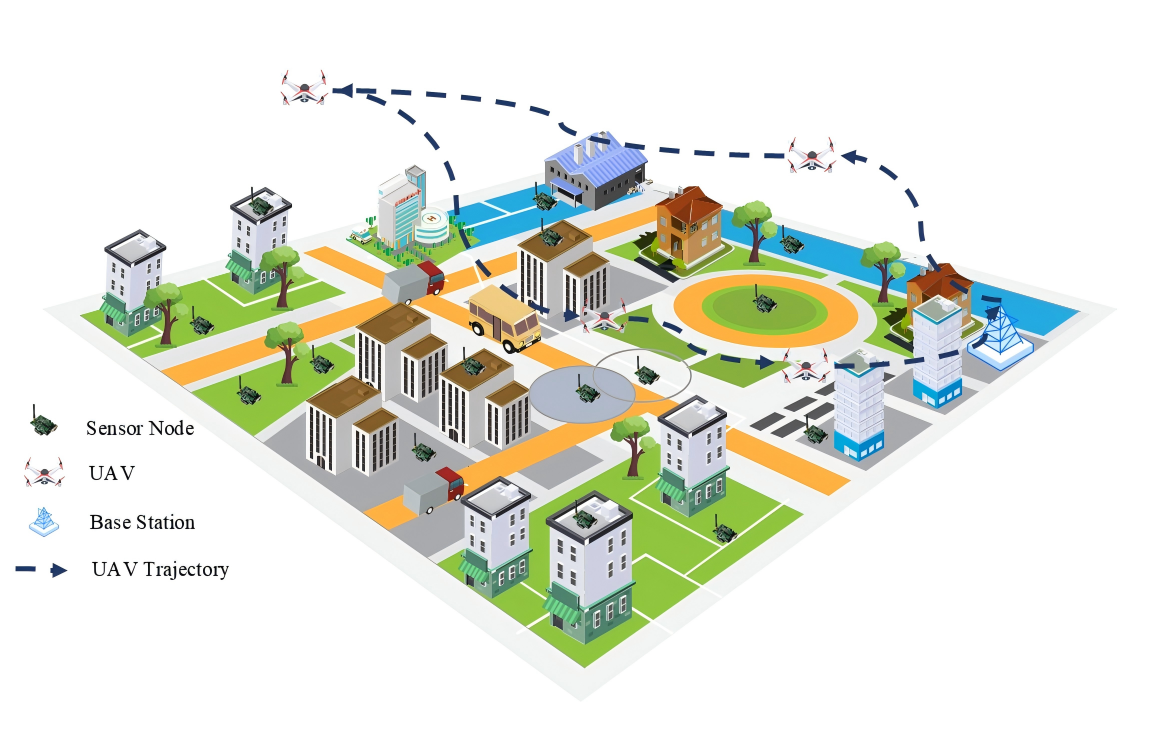
\includegraphics[width=0.45\textwidth]{fig/systemModel.png}
\caption{The UAV-assisted IoT data collection system in a smart city illustrates the distribution of IoT devices with overlapping coverage areas due to their geographical proximity.}


\label{fig:system_model}
\end{figure}

\section{PRELIMINARIES}
\subsection{System Model}
%% 系统模型图

%%在本文中,我们考虑一个由无人机(UAV)和 $n$ 个传感器节点组成的UAV辅助物联网网络,应用于智慧城市或环境监测等场景。传感器节点集合记为 $V=\{v_1,v_2,\ldots,v_n\}$ ,其中传感器节点 $v_i$ 的坐标表示为 $(x_i,y_i,0)$,$1 \leq i \leq n$。
%%为了减少冗余数据的收集并节省无人机的能耗,我们将这 $n$ 个传感器节点划分为 $K$ 个集群,每个集群由一个主传感器节点和若干从传感器节点组成。无人机将在每个集群的主传感器节点上方的高度 $H$ 处进行数据采集。因此,我们确定了悬停点集合 $\mathcal{C}=\{c_1,c_2,\ldots,c_K\}$,其中悬停点 $c_k$ 的坐标为 $(x_{k}^{'},y_{k}^{'},H)$,对应于 $K$ 个集群 $Q_1,Q_2,\ldots,Q_{K}$。
%%在该网络中,无人机按照预定轨迹进行调度,收集传感器节点生成的数据。无人机从起点出发,以恒定速度 $v$ 飞行至某一悬停点后进行数据采集。由于无人机的能量有限,它无法从所有传感器节点收集数据。相反,它仅收集非冗余数据。完成任务后,无人机返回起点进行能量的补充。
%%对于任何一个集群 $Q_i$,无人机可以从主传感器和从传感器收集数据。当无人机悬停在集群 $Q_i$ 上方时,该集群中的主传感器首先将数据发送给无人机。与此同时,其他从传感器节点监听主传感器的传输内容,能够识别出哪些数据是重复的。因此,在向无人机传输数据时,从传感器只需发送其非冗余的数据部分。这样,有效地减少了数据冗余,提高了能量利用效率。
We consider a UAV-assisted IoT network consisting of a UAV and $n$ IoT devices, applied to scenarios such as smart cities or environmental monitoring. The set of IoT devices is denoted as $V=\{v_1,v_2,\ldots,v_n\}$, where the coordinates of IoT device $v_i$ are represented as $(x_i,y_i,0)$, for $1 \leq i \leq n$.

To optimize UAV energy consumption and minimize redundant data collection, we partition the $n$ IoT devices into $K$ clusters, each comprising one main IoT device and multiple subordinate devices. The UAV will collect data at a height $H$ above the main IoT device of each cluster. Consequently, we define a set of waypoints $\mathcal{C}=\{c_1,c_2,\ldots,c_K\}$, where the coordinates of waypoint $c_k$  are $(x_{k}^{'},y_{k}^{'},H)$, corresponding to the $K$ clusters $Q_1,Q_2,\ldots,Q_{K}$.



Within this network, the UAV is scheduled to follow predetermined trajectory, gathering data generated by IoT devices. Departing from the starting point, the UAV flies at a constant velocity $v$ to a designated waypoint where it conducts data collection. Due to the UAV's limited energy, it is unable to collect data from all IoT devices. Instead, it selectively gathers non-redundant data. Upon completing its mission, the UAV returns to the starting point for energy replenishment.

For any given cluster $Q_i$, the UAV can collect data from both the primary and secondary sensors. When the UAV hovers above cluster $Q_i$, the primary sensor within that cluster first transmits its data to the UAV. Simultaneously, the secondary IoT devices listen to the primary sensor's transmission, enabling them to identify which data is redundant. Consequently, when transmitting data to the UAV, the secondary sensors only need to send their non-redundant portions. This approach effectively reduces data redundancy and enhances energy efficiency.

% Journals use one of three template styles. All but three ACM journals
% use the {\verb|acmsmall|} template style:
% \begin{itemize}
% \item {\texttt{acmsmall}}: The default journal template style.
% \item {\texttt{acmlarge}}: Used by JOCCH and TAP.
% \item {\texttt{acmtog}}: Used by TOG.
% \end{itemize}

% The majority of conference proceedings documentation will use the {\verb|acmconf|} template style.
% \begin{itemize}
% \item {\texttt{sigconf}}: The default proceedings template style.
% \item{\texttt{sigchi}}: Used for SIGCHI conference articles.
% \item{\texttt{sigplan}}: Used for SIGPLAN conference articles.
% \end{itemize}

\subsection{Spatial Data Correlation Model}
%%在无线传感器网络中,地理上相邻的传感器可能同时具有相似的传感数据。根据[7]中的研究,空间数据相关性$c(i,j)$是通过计算传感器$v_i$和 $v_j$ 在同一时间段内数据相似度。用公式表示如下:$$c(i,j)=\frac{N_{i,j}}{N}$$

%%其中$N$表示在一段固定的时间段内划分的时间槽数,$N_{i,j}$表示在$N$个时间槽中,传感器$v_i$和$v_j$之间的数据差异不超过阈值$γ$的时间槽的数量。

%%为了从网络中的$n$个传感器收集非冗余信息,,我们将网络中的n个传感器节点划分成$K$个不相交的集群$Q_1,Q_2,\ldots,Q_{K}$。每个集群包含一个主传感器和若干从传感器。当无人机在某个集群中收集数据时,主传感器会将所有数据传输给无人机,而从传感器则仅传输非冗余的数据。这样,将从每个集群中收集更少的冗余数据,从而降低无人机的能量消耗,并使其能够收集更多节点的数据。

%%我们应用[7]中的方法,来将网络中的n个传感器节点进行集群的划分。其中集群的个数$K$没有给出,由数据相关性关系所决定。具体来说,设$u_i$是集群$Q_i$的主传感器,则$u_i$与该集群中的其他从传感器$v_j$之间的冗余数据量可以表示为$$P_{ij}=\min\{D_{i}^{Q},D_{j}^{Q}\}\cdot c(i,j)$$

%%需要注意的是,这一计算方式与文献[7]中的方法有所不同。在文献[7]中,如果主传感器收集的数据量过大,而从传感器收集的数据量较少,可能会导致计算出的主从节点之间的冗余数据量超过从节点实际收集的总数据量。虽然我们这一修改可能会导致计算的冗余数据量少于真实的冗余数据量,但我们有效避免了上述问题。因此,确定好主传感器节以及附属点后网络中的冗余数据传输总量为$$\sum_{i=1}^K\sum_{v_j\in Q_i\setminus\{u_i\}}P_{ij}$$

In wireless sensor networks, geographically adjacent sensors may have similar sensor data. According to the study in \cite{8-Minimizing_redundant}, the spatial data correlation $c(i,j)$ is calculated by evaluating the data similarity between sensor $v_i$ and sensor $v_j$ over the same time period. This can be expressed by the following formula:

\begin{equation}
    c(i,j)=\frac{N_{i,j}}{N},
\end{equation}
where $N$ represents the number of time slots within a fixed time period, and $N_{i,j}$ denotes the number of time slots in which the data difference between sensor $v_i$ and sensor $v_j$ does not exceed the threshold $\gamma$ over the $N$ time slots.

To collect non-redundant information from the $n$ sensors in the network, we partition the $n$ IoT devices in the network into $K$ disjoint clusters $Q_1,Q_2,\ldots,Q_{K}$. Each cluster contains a main sensor and several subordinate sensors. When the UAV collects data in a cluster, the main sensor transmits all data to the UAV, while subordinate sensors only transmit their non-redundant data. This reduces the amount of redundant data collected from each cluster, thereby lowering the energy consumption of the UAV and enabling it to collect more data from the IoT devices.

We apply the method from \cite{8-Minimizing_redundant} to partition the $n$ IoT devices in the network into clusters. The number of clusters $K$ is not predetermined but is determined by the data correlation relationship. Specifically, let $u_i$ be the main sensor of cluster $Q_i$. The redundant data between $u_i$ and subordinate sensors $v_j$ in the same cluster can be expressed as:
\begin{equation}
    r_{ij}=\min\{D_{i}^{Q},D_{j}^{Q}\}\cdot c(i,j).
\end{equation}

It is important to note that our calculation method differs from \cite{8-Minimizing_redundant}, where if the data collected by the main sensor is significantly larger than that collected by subordinate sensors, the calculated redundant data between them may exceed the total data collected by the subordinate sensors. Our approach, while potentially underestimating the actual redundancy, effectively avoids this issue. Therefore, after determining the main sensor and subordinate IoT devices, the total amount of redundant data transmission in the network is given by:
\begin{equation}
    \sum_{i=1}^K\sum_{v_j\in Q_i\setminus\{u_i\}}r_{ij}.
\end{equation}

\subsection{UAV Model}

%%在不失一般性的情况下,我们假设无人机以固定的速 $v_{\mathrm{uav}}$ 从一个悬停点飞往另一个悬停点。无人机的推进能耗由[无人机能耗模型]给出: 
%%$$\begin{aligned}P_{\mathrm{mov}}(v_{\mathrm{uav}})&=P_0\left(1+\frac{3v_{\mathrm{uav}}^2}{U_{\mathrm{tip}}^2}\right)+P_1\left(\left(1+\frac{v_{\mathrm{uav}}^4}{4v_0^4}\right)^{1/2}\right.\\&-\left.\frac{v_{\mathrm{uav}}^2}{2v_0^2}\right)^{1/2}+\frac12d_0\rho s\delta v_{\mathrm{uav}}^3\end{aligned}$$

%%其中,$P_0$和$P_1$是定义的两个常数,分别表示悬停状态下的桨叶轮廓功率和诱导功率,$U_{tip}$表示桨叶尖速度,$v_0$是已知的悬停状态下的平均旋翼诱导速度,$d_0$和$s$分别是机身阻力比和旋翼刚度,$\rho$和$\delta$分别表示空气密度和旋翼盘面积。

%%当无人机在集群$Q_i$上方悬停点$c_i$收集数据时,其在悬停状态下的功耗可以通过带入$v_{uav}=0$来获得。此外,如果无人机在收集数据时的悬停高度 $H$ 相对较低,则集群中主传感器节点与其从传感器节点之间向无人机传输数据的速率差异可以忽略不计。为简化讨论,我们假设一个集群中的所有传感器节点具有相同的传输速率。同时,我们假设无人机的悬停时间等于数据的传输时间。因此,其能耗可以表示为:
%%$$E_{c_k}=\frac{D_i}{r_\text{data}}(P_\text{hover}+P_\text{com})$$

%%其中,$D_i$表示无人机在悬停点$c_i$处收集的数据量。$P_{com}$代表无人机的通信功率。无人机从悬停点$c_i$移动到另一个悬停点$c_j$所消耗的能量可以表示为:
%%$$E_{{c_{i},c_{j}}}=\frac{\|c_{i}-c_{j}\|}{v_{{\mathrm{uav}}}}P_{{\mathrm{move}}}$$

%%其中$\|c_i-c_j\|$代表悬停点$c_i$和$c_j$之间的直线距离。所以无人机在飞行过程中的总能耗可以表示为:
%%$$\begin{aligned}E_{\mathrm{flight}}& =\sum_{i=0}^K\sum_{j=0}^KE_{c_i,c_j}L_{c_i,c_j} \\&=\sum_{i=0}^K\sum_{j=0}^K\frac{L_{ci,ci}||c_{i}-c_{j}||P_{0}}{v_{uav}}(1+\frac{3v_{uav}^{2}}{U_{tip}^{2}}) \\&+\sum_{i=0}^K\sum_{j=0}^K\frac{L_{c_i,c_i}\|c_i-c_j\|P_{1}}{v_{uav}}((1+\frac{v_{wav}^{4}}{4v_{0}^{4}})^{1/2}-\frac{v_{wav}^{2}}{2v_{0}^{2}})^{1/2}\\&+\sum_{i=0}^K\sum_{j=0}^K\frac{L_{ci,cj}||c_{i}-c_{j}||d_{0}\rho s\delta v_{uav}^{2}}{2}\end{aligned}$$
%%$\mathcal{C}=\{c_1,c_2,\ldots,c_K\}$表示悬停点的集合,$L_{c_i,c_j}$表示无人机是否从$c_i$移动到$c_j$。具体的定义如下:
%%$$L_{{c_{i},c_{j}}}=\begin{cases}1,&\text{the path goes from}c_{i}\text{to}c_{j}\\0,&\text{otherwise.}&&\end{cases}$$
Without loss of generality, we assume that the UAV flies from one waypoint to another at a constant speed $v_{\mathrm{uav}}$. The propulsion energy consumption of the UAV is given by the \cite{13-UavenergyModel}: 
\begin{equation}
    \ \begin{aligned}P_{\mathrm{mov}}(v_{\mathrm{uav}})&=P_0\left(1+\frac{3v_{\mathrm{uav}}^2}{U_{\mathrm{tip}}^2}\right)+P_1\left(\left(1+\frac{v_{\mathrm{uav}}^4}{4v_0^4}\right)^{1/2}\right.\\&-\left.\frac{v_{\mathrm{uav}}^2}{2v_0^2}\right)^{1/2}+\frac12d_0\rho s\delta v_{\mathrm{uav}}^3\end{aligned},
\end{equation}
where $P_0$ and $P_1$ are predefined constants representing the profile power and induced power of the rotor blades in hover, respectively; $U_{tip}$ denotes the blade tip speed; $v_0$ is the known average rotor-induced velocity in hover; $d_0$ and $s$ represent the body drag coefficient and rotor stiffness, respectively; $\rho$ is the air density, and $\delta$ refers to the rotor disk area. 

When the UAV collects data at the waypoint $c_i$ located above cluster $Q_i$, the power consumption during hovering can be obtained by substituting $v_{uav}=0$ into the equation. Furthermore, if the UAV's hovering altitude $H$ is relatively low, the variation in data transmission rates between the main IoT device and its subordinate devices within the cluster can be considered negligible. To simplify the discussion, we assume that all IoT devices in a cluster have identical transmission rates. Additionally, the UAV's hovering time is assumed to be equal to the data transmission time. Accordingly, the energy consumption during data collection can be expressed as:


\begin{equation}
     E_{c_k}=\frac{D_{i}^{nr}}{r_\text{data}}(P_\text{hover}+P_\text{com}),
\end{equation}
where $D_{i}^{nr}$ represents the amount of non-redundant data collected by the UAV at the waypoint $c_i$, and $P_{com}$ denotes the communication power of the UAV.
The energy consumption of the UAV when moving from waypoint $c_i$ to another waypoint $c_j$ can be represented as:
\begin{equation}
     E_{{c_{i},c_{j}}}=\frac{\|c_{i}-c_{j}\|}{v_{{\mathrm{uav}}}}P_{{\mathrm{move}}},
\end{equation}
where $\|c_i-c_j\|$ denotes the Euclidean distance between waypoints $c_i$ and $c_j$. Let $\mathcal{C}=\{c_1,c_2,\ldots,c_K\}$ denote the collection of waypoints, and $L_{c_i,c_j}$ indicate whether the UAV travels from $c_i$ to $c_j$. The specific definition of $L_{c_i,c_j}$ is given as:


\begin{equation}
     L_{{c_{i},c_{j}}}=
\begin{cases}
1, & \text{if the path goes from } c_{i} \text{ to } c_{j}. \\
0, & \text{otherwise.}
\end{cases}
\end{equation}

\subsection{Communication Model}
%%在从设备节点之间收集数据之前,无人机必须逐个与每个节点建立可靠的连接。在本文中,我们关注的是无人机在悬停时收集数据的情况。考虑两种类型的通信链路,一种是视线(LoS),另一个是非视线(NLoS)。当飞行高度较高时,其障碍物较少,使用LoS链路。否则使用NLoS链路。LoS链路的概率通常由以下公式给出:
%%$$P_{LoS}=\frac{1}{1+a\exp\left(-b\left[\frac{180}{\pi}\arcsin\left(\frac{H}{d_{i,k}}\right)-a\right]\right)}$$
%%其中$a,b$是与环境相关的两个参数,$d_{i,k}$是无人机在悬停点处与设备节点之间的距离。同时,NLoS链路的概率可以表示为$P_{NLoS} = 1 - P_{LoS}$。每个节点和无人机之间的平均路径损耗可以表示为 
%%$$\overline{P}_{\mathrm{loss}}=P_{\mathrm{LoS}}\left(K_0+\mu_{\mathrm{LoS}}\right)+P_{\mathrm{NLoS}}\left(K_0+\mu_{\mathrm{NLoS}}\right)$$
%%其中,$\mu_{\mathrm{LoS}}$和$\mu_{\mathrm{NLoS}}$分别是LOS和NLOS链路中过度路径损耗的平均值,$K_0=10\alpha\log_{10}(\frac{4\pi f_{c}H}{c})$,$\alpha$是路径损耗指数,$c$是光速,$f_{c}$是载波频率。因此,每个节点到无人机的平均数据传输速率可以通过以下的公式计算
%%$$r_{\mathrm{data}}=B_{\mathrm{width}}\log_2\left(1+\frac{P_{trans}}{\overline{P}_{\mathrm{loss}}N_0}\right)$$
%%其中,$B_{\mathrm{width}}$是可用的带宽,$N_0$是噪声功率谱密度,$P_{trans}$是每个节点的传输功率。
Before collecting data from the IoT devices, the UAV must first establish a reliable connection with each IoT device. In this paper, we focus on data collection by the UAV during hovering. Two types of communication links are considered: Line-of-Sight (LoS) and Non-Line-of-Sight (NLoS). When the UAV is flying at a higher altitude, fewer obstacles are present, and an LoS link is used. Otherwise, an NLoS link is employed. The probability of an LoS link is typically given by the following formula:


\begin{equation}
    P_{\text{LoS}}=\frac{1}{1+a\exp\left(-b\left[\frac{180}{\pi}\arcsin\left(\frac{H}{d_{i,k}}\right)-a\right]\right)},
\end{equation}
where $a$ and $b$ are two environment-dependent parameters, and $d_{i,k}$ is the distance between the UAV's waypoint and the IoT devices. Meanwhile, the probability of an NLoS link is given by $P_{\text{NLoS}} = 1 - P_{\text{LoS}}$. The average path loss between each IoT device and the UAV can be expressed as:

\begin{equation}
    \overline{P}_{\mathrm{loss}}=P_{\mathrm{LoS}}\left(K_0+\mu_{\mathrm{LoS}}\right)+P_{\mathrm{NLoS}}\left(K_0+\mu_{\mathrm{NLoS}}\right),
\end{equation}
where $\mu_{\mathrm{LoS}}$ and $\mu_{\mathrm{NLoS}}$ represent the average excess path loss for LoS and NLoS links, respectively, and $K_0=10\alpha\log_{10}(\frac{4\pi f_{c}H}{c})$, where $\alpha$ is the path loss exponent, $c$ is the speed of light, and $f_{c}$ is the carrier frequency. Therefore, the average data transmission rate between each IoT device and the UAV can be calculated using the following formula:

\begin{equation}
    r_{\mathrm{data}}=B_{\mathrm{width}}\log_2\left(1+\frac{P_{trans}}{\overline{P}_{\mathrm{loss}}N_0}\right),
\end{equation}
where $B_{\mathrm{width}}$ is the available bandwidth, $N_0$ is the noise power spectral density, and $P_{trans}$ is the transmission power of IoT devices.



\section{Problem Formulation}
%%【定义原始优化目标】-【划分成两个子问题】-【P1:传感器节点的聚类】-【P2:根据聚类结果规划无人机路径】
% 在本文中,我们的目标是通过无人机收集所有传感器节点的数据,并在合理的时间内最小化冗余数据的收集和能量消耗。优化目标可表示为:
% $$\mathcal{P}_1:\quad\min_{\mathcal{U},\Pi,\mathbf{P}} \left[\sum_{i=1}^K R_{\mathrm{collect}}^i(\mathbf{P}) + E_{\mathrm{hover}}(\mathbf{P}) + E_{\mathrm{flight}}(\Pi,\mathcal{U})\right]$$
% 公式中的 $\mathcal{U}$ 表示无人机在数据收集过程中所选的悬停点集合,$\Pi$代表无人机访问这些悬停点的顺序,而 $\mathbf{P}$ 则反映了不同传感器节点之间的数据相似性。通过优化上述公式,我们能够最小化冗余数据收集和能量消耗。
% 冗余数据收集 $\sum_{i=1}^K R_{\mathrm{collect}}^i(\mathbf{P})$ 和悬停能耗 $E_{\mathrm{hover}}(\mathbf{P})$ 都由节点间的数据相似性矩阵 $\mathbf{P}$ 决定。具体而言,悬停能耗主要受在悬停点处收集的数据量影响,而收集数据量的大小又与 $\mathbf{P}$ 密切相关。此外,数据传输过程中产生的能耗相对较小。因此,在优化目标时,这两部分能耗的最小化主要依赖于 $\mathbf{P}$,而与无人机的飞行路径 $\Pi$ 和悬停点集合 $\mathcal{U}$ 无关。
In this paper, our objective is to collect data from all IoT devices using a UAV while minimizing redundant data collection and energy consumption within a reasonable time. The optimization goal can be formulated as:
\begin{equation}
    \mathcal{P}_1:\min_{\mathcal{U},\Pi,\mathbf{S}} \left[\sum_{i=1}^K R_{\mathrm{collect}}^i(\mathbf{S}) + E_{\mathrm{hover}}(\mathbf{S}) + E_{\mathrm{flight}}(\Pi,\mathcal{U})\right],
\end{equation}
where $\mathcal{U}$ represents the set of waypoints selected by the UAV during data collection, $\Pi$ denotes the visiting sequence of these waypoints, and $\mathbf{S}$ characterizes the data similarity between different IoT devices. By optimizing the above equation, we aim to minimize both redundant data collection and energy consumption. The amount of redundant data collected, $\sum_{i=1}^K R_{\mathrm{collect}}^i(\mathbf{S})$, and the hovering energy consumption, $E_{\mathrm{hover}}(\mathbf{S})$, are both determined by the data similarity matrix $\mathbf{S}$. Specifically, the hovering energy consumption is primarily influenced by the amount of data collected at each waypoint, which is closely related to $\mathbf{S}$. Moreover, the energy consumption incurred during data transmission is relatively small. Therefore, in the optimization objective, the minimization of these two energy-related components mainly depends on $\mathbf{S}$ and is independent of the UAV's flight trajectory $\Pi$ and the set of waypoints $\mathcal{U}$. Thus, the original optimization problem can be decomposed as:
\begin{equation}
\begin{aligned}
\min_{\mathcal{U},\Pi,\mathbf{S}} \; &\Biggl[\sum_{i=1}^K R_{\mathrm{collect}}^i(\mathbf{S}) 
+ E_{\mathrm{hover}}(\mathbf{S}) + E_{\mathrm{flight}}(\Pi,\mathcal{U})\Biggr] \\
=&\;\min_{\mathbf{S}} \Biggl[\sum_{i=1}^K R_{\mathrm{collect}}^i(\mathbf{S}) 
+ E_{\mathrm{hover}}(\mathbf{S})\Biggr]+\min_{\mathcal{U},\Pi} E_{\mathrm{flight}}(\Pi,\mathcal{U})  
\end{aligned}
\end{equation}

% 因此,原始的优化问题可以表述为:
% $$
% \begin{aligned}
% \min_{\mathcal{U},\Pi,\mathbf{P}} \; &\Biggl[\sum_{i=1}^K R_{\mathrm{collect}}^i(\mathbf{P}) 
% + E_{\mathrm{hover}}(\mathbf{P}) + E_{\mathrm{flight}}(\Pi,\mathcal{U})\Biggr] \\
% =&\;\min \Biggl[\sum_{i=1}^K R_{\mathrm{collect}}^i(\mathbf{P}) 
% + E_{\mathrm{hover}}(\mathbf{P})\Biggr]+\min E_{\mathrm{flight}}(\Pi,\mathcal{U})  \\
% \end{aligned}
% $$

%将公式(4)(5)(6)(7)代入上述可以得到

% $$
% \begin{aligned}
% \min_{\mathcal{U},\Pi,\mathbf{P}} \; &\Biggl[\sum_{i=1}^K R_{\mathrm{collect}}^i(\mathbf{P}) 
% + E_{\mathrm{hover}}(\mathbf{P}) + E_{\mathrm{flight}}(\Pi,\mathcal{U})\Biggr] \\

% =&\; \min \sum_{i=0}^{K}\sum_{j=0}^{K} L_{c_i,c_j}\,\|c_{i}-c_{j}\|\Biggl[\frac{P_{0}}{v_{uav}}
% +\frac{3P_{0}v_{uav}}{U_{tip}^{2}}\\
% &+\;\frac{P_{1}}{v_{uav}}
% \Biggl(\sqrt{1+\frac{v_{uav}^{4}}{4v_{0}^{4}}}-\frac{v_{uav}^{2}}{2v_{0}^{2}}\Biggr)^{\frac{1}{2}}
% +\frac{d_{0}\rho s\delta v_{uav}^{2}}{2}\Biggr] \\
% &+\; \min \Biggl[\sum_{i=1}^{K} \frac{D_{i}^{}}{r_{data}}\,(P_0+P_1+P_{com})+ R_{\mathrm{collect}}^i \Biggr]\\
% \end{aligned}
% $$
By substituting equations (4), (5), (6), and (7) into the above formulation, we obtain:
\begin{equation}
    \begin{aligned}
    \min_{\mathcal{U},\Pi,\mathbf{S}} \; &\Biggl[\sum_{i=1}^K R_{\mathrm{collect}}^i(\mathbf{S}) 
    + E_{\mathrm{hover}}(\mathbf{S}) + E_{\mathrm{flight}}(\Pi,\mathcal{U})\Biggr] \\
    =&\; \min \sum_{i=0}^{K}\sum_{j=0}^{K} L_{c_i,c_j}\,\|c_{i}-c_{j}\|\Biggl[\frac{P_{0}}{v_{\mathrm{uav}}}
    + \frac{3P_{0}v_{\mathrm{uav}}}{U_{\mathrm{tip}}^{2}} \\
    &+ \frac{P_{1}}{v_{\mathrm{uav}}} \Biggl( \sqrt{1 + \frac{v_{\mathrm{uav}}^{4}}{4v_{0}^{4}}} - \frac{v_{\mathrm{uav}}^{2}}{2v_{0}^{2}} \Biggr)^{\frac{1}{2}}
    + \frac{d_{0}\rho s\delta v_{\mathrm{uav}}^{2}}{2} \Biggr] \\
    &+ \min \Biggl[\sum_{i=1}^{K} \frac{D_{i}}{r_{\mathrm{data}}}\,(P_0 + P_1 + P_{\mathrm{com}}) + R_{\mathrm{collect}}^i \Biggr]
    \end{aligned}
\end{equation}
%同时我们用$f(v_{uav})$来替代$\frac{P_{0}}{v_{uav}}+\frac{3P_{0}v_{uav}}{U_{tip}^{2}}+\frac{P_{1}}{v_{uav}}((1+\frac{v_{uav}^{4}}{4v_{0}^{4}})^{\frac{1}{2}}-\frac{v_{uav}^{2}}{2v_{0}^{2}})^{\frac{1}{2}}+\frac{d_{0}\rho s\delta v_{uav}^{2}}{2}$,则上述的公式可以表示为
%$$
%\begin{aligned}
%\min_{\mathcal{U},\Pi,\mathbf{P}} \; &\Biggl[\sum_{i=1}^K R_{\mathrm{collect}}^i(\mathbf{P}) 
%+ E_{\mathrm{hover}}(\mathbf{P}) + E_{\mathrm{flight}}(\Pi,\mathcal{U})\Biggr] \\
%=&\; \min \sum_{i=0}^{K}\sum_{j=0}^{K} L_{c_i,c_j}\,\|c_{i}-c_{j}\|f(v_{uav}) \\
%&+\; \min \Biggl[\sum_{i=1}^{K} \frac{D_{i}^{}}{r_{data}}\,(P_0+P_1+P_{com})+ %R_{\mathrm{collect}}^i \Biggr]\\
%\end{aligned}
%$$
To simplify the notation, we define $f(v_{uav})$ as follows:
\begin{equation}
\begin{aligned}
    f(v_{\mathrm{uav}}) = & \frac{P_0}{v_{\mathrm{uav}}} + \frac{3P_0 v_{\mathrm{uav}}}{U_{\mathrm{tip}}^2} \\
    & + \frac{P_1}{v_{\mathrm{uav}}} \left( \left( 1 + \frac{v_{\mathrm{uav}}^4}{4v_0^4} \right)^{\frac{1}{2}} - \frac{v_{\mathrm{uav}}^2}{2v_0^2} \right)^{\frac{1}{2}} \\
    & + \frac{d_0 \rho s \delta v_{\mathrm{uav}}^2}{2}
\end{aligned}
\end{equation}
%从上述公式可以看出,最小化冗余数据收集与能量消耗,与无人机的飞行路径长度及网络中被抑制传输的冗余数据量密切相关。被抑制的冗余数据量越大,收集的冗余数据量就越少。在总数据量固定的情况下,抑制的冗余数据量增加,收集的数据量相应减少。为解决该问题,我们将其分解为两个子问题。首先,基于传感器节点之间的数据相关性进行聚类,以确定无人机的悬停点集合 $\mathcal{U}$,从而尽可能减少网络中冗余数据的传输。其次,根据聚类结果对无人机的悬停点进行轨迹调度,优化其飞行轨迹 $\Pi$。在下一节,我们将详细介绍这两个子问题的具体处理方法。
Thus, the optimization problem can be rewritten as:
\begin{equation}
\begin{aligned}
\min_{\mathcal{U}, \Pi, \mathbf{S}} \; & \Biggl[ \sum_{i=1}^{K} R_{\mathrm{collect}}^i(\mathbf{S}) + E_{\mathrm{hover}}(\mathbf{S}) + E_{\mathrm{flight}}(\Pi, \mathcal{U}) \Biggr] \\
=& \; \min \sum_{i=0}^{K} \sum_{j=0}^{K} L_{c_i, c_j} \, \|c_i - c_j\| f(v_{\mathrm{uav}}) \\
& + \; \min \Biggl[ \sum_{i=1}^{K} \frac{D_i}{r_{\mathrm{data}}} (P_0 + P_1 + P_{\mathrm{com}}) + R_{\mathrm{collect}}^i \Biggr]
\end{aligned}
\end{equation}

From the above formula, it is evident that minimizing redundant data collection and energy consumption is closely related to both the flight distance of the UAV and the amount of redundant data suppressed from transmission within the network. The greater the suppressed redundant data, the less redundant data is collected. Given a fixed total data volume, an increase in the suppressed redundant data leads to a corresponding reduction in the collected data volume. To address this issue, we decompose it into two subproblems. First, clustering is conducted based on the data correlation among IoT devices to determine the set of UAV waypoints $\mathcal{U}$, thereby aiming to minimize redundant data transmission within the network. Secondly, based on the clustering results, the waypoints of the UAV are scheduled to optimize its flight trajectory, denoted as $\Pi$. In the next section, we will elaborate on the specific methods for addressing these two subproblems.


\section{SOLUTION METHOD}
%%MISRED: Maximizing the Suppression of Network Redundancy


% UTICA:Path Planning Using GCN and MCTS

\subsection{Maximizing the Suppression of Network Redundancy}
%在本节中,我们提出了一种优化无人机悬停点选择的算法 MISRED,旨在最大化网络中被抑制传输的冗余数据量。该算法的核心目标是将所有传感器节点划分为 $K$ 个专属集群 $Q_1, Q_2, \dots, Q_K$,并在每个集群 $Q_i$ 中选取一个主传感器节点,以最大程度地减少冗余数据的传输,从而降低无人机在悬停数据收集过程中的能耗。随后,根据这些主传感器节点的位置,确定无人机的 $K$ 个悬停点,以优化其数据收集效率。数学上,该优化过程可表示为:
%%$$\mathcal{P}_2:\quad\max_{M\subseteq V}\{f(M)\}=\max_{M\subseteq V}\left\{\sum_{v_j\in V\setminus M}\max_{v_i\in M}\{r_{ij}\}\right\}.$$
%%请注意问题$\mathcal{P}_2$是一个无约束的子模最大化问题,并且已被证明是一个 NP -hard问题(见文献 [7]),其中约束16a表示传感器节点通信范围的限制。正如文献 [7] 中所述,网络中冗余数据抑制最大化问题等价于找到一组主传感器 $M \subseteq V$ 使得 $\mathcal{P}_2$ 成立。基于此性质,我们提出了一种用于确定悬停点的算法。该算法通过最大化冗余数据抑制来优化悬停位置的选择,并且可以在$1-(1/n^\alpha)$的概率下提供一个$(0.5-\epsilon)$近似解,其中$\epsilon$和 $\alpha$ 是两个给定的常数,满足 0<$\epsilon$≤0.5  且$\alpha$>0。



In this section, we propose an algorithm named MISRED\footnote{The name MISRED comes from \underline{M}ax\underline{I}mizing the \underline{S}uppression of Network \underline{RED}undancy.} for optimizing the selection of waypoints for UAVs, aiming to maximize the suppression of redundant data transmission in the network. The primary objective of this algorithm is to partition all IoT devices into $K$ dedicated clusters, denoted as $Q_1, Q_2, \dots, Q_K$, and select a representative IoT device within each cluster $Q_i$ to minimize redundant data transmissions. This approach effectively reduces the energy consumption of the UAV during the hovering-based data collection process. Subsequently, the UAV's $K$ waypoints are determined based on the locations of these representative IoT devices to optimize data collection efficiency. Mathematically, this optimization process can be formulated as:



\begin{equation}
    \mathcal{P}_2:\quad\max_{M\subseteq V}\{f(M)\}=\max_{M\subseteq V}\left\{\sum_{v_j\in V\setminus M}\max_{v_i\in M}\{r_{ij}\}\right\},
\end{equation}
subject to the communication range constraint that ensures connectivity between IoT devices within each cluster.
% \begin{subequations} \label{eq:P2}
% \begin{align}
% & r_{\text{com}} \leq r_{\text{max}},  && \label{eq:P2a} \tag{16a} 
% \end{align}
% \end{subequations}
% \setcounter{equation}{16}

The problem $\mathcal{P}_2$ is an unconstrained submodular maximization problem, which has been proven to be NP-hard \cite{8-Minimizing_redundant}. According to this research, maximizing redundant data suppression in the network is equivalent to selecting a set of primary sensors $M \subseteq V$ such that $\mathcal{P}_2$ holds. Leveraging this equivalence, we propose MISRED to optimize the selection of UAV waypoints. 
% The MISRED algorithm determines the hovering locations by maximizing redundant data suppression and guarantees a $(0.5-\epsilon)$-approximate solution with at least $1-(1/n^\alpha)$ probability, where $\epsilon$ and $\alpha$ are given constants satisfying $0 < \epsilon \leq 0.5$ and $\alpha > 0$.
Algorithm 1 details the MISRED approach. The algorithm takes as input the set of IoT devices, the amount of suppressed redundant data transmissions when assigning master-slave relationships, an error ratio $\epsilon$, and a desired success probability. MISRED operates through an iterative probabilistic process over $L$ iterations. In each iteration, the algorithm evaluates each device's potential contribution to the objective function by calculating its marginal gain when added to the master set and its marginal loss when removed from consideration. Based on these values, it makes probabilistic decisions to either include devices in the master set or exclude them. For each non-master device, MISRED assigns a master device that maximizes redundant data suppression. Finally, it determines the optimal UAV waypoints directly above the selected master devices at a predetermined height $H$. %This approach effectively balances data collection requirements while minimizing network redundancy.



% \algrenewcommand{\algorithmicrequire}{\textbf{Input:}}  % 修改 Input 关键字
% \algrenewcommand{\algorithmicensure}{\textbf{Output:}}  % 修改 Output 关键字
% \begin{algorithm}
% \caption{MISRED: Maximizing the Suppression of Network Redundancy}
% \begin{algorithmic}[1]
% \Require IoT devices $v_1, v_2, \ldots, v_n$, the amount $p_{ij}$ of suppressed redundant data transmissions by sensor $v_j$ if $v_i$ is its master IoT device, an error ratio $\epsilon$ with $0 < \epsilon \leq 0.5$, and a success probability $1 - \frac{1}{n^\alpha}$.
% \Ensure Master IoT device set $M$ and waypoint set $C$.
% \State Let $L = \epsilon \cdot \log_{1 + 2\epsilon} n$;
% \State Let $M = \emptyset$ and $N_0 = V$; 
% \For{$l \gets 1$ to $L$}
%     \For{$i \gets 1$ to $n$} 
%         \State $a_i = f(M_{i-1} \cup \{v_i\}) - f(M_{i-1})$; 
%         \State $\tilde{a}_i = \max\{a_i, 0\}$; 
%         \State $b_i = f(N_{i-1} \setminus \{v_i\}) - f(N_{i-1})$; 
%         \State $\tilde{b}_i = \max\{b_i, 0\}$; 
%         \State Add $v_i$ to $M_{i-1}$ with probability $\frac{\tilde{a}_i}{\tilde{a}_i + \tilde{b}_i}$ or remove $v_i$ from $N_{i-1}$ with probability $1 - \frac{\tilde{a}_i}{\tilde{a}_i + \tilde{b}_i}$; 
%     \EndFor
%     \State $M^{(l)} = M$;
%     \For{each $v_j \in V \setminus M$} 
%         \State $u = \arg \max_{v_i \in M} \{p_{ij}\}$; 
%     \EndFor 
%     \If{$f(M^{(l)}) > f(M)$}
%         \State $M \gets M^{(l)}$;
%     \EndIf
% \EndFor
% \State $C=\{(x_k', y_k', H) \mid \text{waypoints for IoT devices in } M\}$;

% \State \Return the sets of master IoT devices $M$ and waypoints $C$;
% \end{algorithmic}
% \end{algorithm}

\algrenewcommand{\algorithmicrequire}{\textbf{Input:}}  % 修改 Input 关键字
\algrenewcommand{\algorithmicensure}{\textbf{Output:}}  % 修改 Output 关键字
\begin{algorithm}
\caption{MISRED: Maximizing the Suppression of Network Redundancy}
\begin{algorithmic}[1]
\Require IoT devices $v_1, v_2, \ldots, v_n$, the amount $p_{ij}$ of suppressed redundant data transmissions by sensor $v_j$ if $v_i$ is its master IoT device, an error ratio $\epsilon$ with $0 < \epsilon \leq 0.5$, and a success probability $1 - \frac{1}{n^\alpha}$.
\Ensure Master IoT device set $M$ and waypoint set $C$.
\State Let $L = \epsilon \cdot \log_{1 + 2\epsilon} n$;
\State Let $M = \emptyset$ and $N_0 = V$; 
\For{$l \gets 1$ to $L$}
    \State Let $M_0 = M$ and $N_0 = V \setminus M$;
    \For{$i \gets 1$ to $n$} 
        \State $a_i = f(M_{i-1} \cup \{v_i\}) - f(M_{i-1})$; $\tilde{a}_i = \max\{a_i, 0\}$;
        % \State $\tilde{a}_i = \max\{a_i, 0\}$; 
        \State $b_i = f(N_{i-1} \setminus \{v_i\}) - f(N_{i-1})$; $\tilde{b}_i = \max\{b_i, 0\}$; 
        % \State $\tilde{b}_i = \max\{b_i, 0\}$; 
        \State Generate a random number $r \in [0,1]$
            \If{$r \leq \frac{\tilde{a}_i}{\tilde{a}_i + \tilde{b}_i}$}
            \State $M_i = M_{i-1} \cup \{v_i\}$
            \Else
            \State $N_i = N_{i-1} \setminus \{v_i\}$
            \EndIf

    \EndFor
    \State $M^{(l)} = M_n$;
    \For{each $v_j \in V \setminus M^{(l)}$} 
        \State $u = \arg \max_{v_i \in M^{(l)}} \{p_{ij}\}$; 
    \EndFor 
    \If{$f(M^{(l)}) > f(M)$}
        \State $M \gets M^{(l)}$;
    \EndIf
\EndFor
\State $C=\{(x_i, y_i, H) \mid v_i \in M\}$; 
% \Comment{Determine waypoints above master devices}

\State \Return the sets of master IoT devices $M$ and waypoints $C$;
\end{algorithmic}
\end{algorithm}

The MISRED algorithm determines the hovering locations by maximizing redundant data suppression and guarantees a $(0.5-\epsilon)$-approximate solution with at least $1-(1/n^\alpha)$ probability, where $\epsilon$ and $\alpha$ are given constants satisfying $0 < \epsilon \leq 0.5$ and $\alpha > 0$. In terms of computational complexity, MISRED executes $L = \epsilon \cdot \log_{1 + 2\epsilon} n$ iterations, with each iteration requiring $O(n^2)$ operations for calculating marginal gains and losses across all IoT devices. Thus, the overall time complexity of MISRED is $O(n^2 \cdot \log n)$, making it efficient for practical deployment in medium to large-scale IoT networks.


\subsection{Heatmap-Guided Reinforcement Learning Trajectory Optimization}
% 
% UTICA: heatmap-gUided reinforcemenT learnIng trajeCtory optimizAtion
%在求解问题$\mathcal{P}_2$获得无人机的悬停位置后,我们提出一种路径规划算法UTICA来优化无人机的飞行能耗。无人机需要从起点开始遍历所有的悬停点进行数据的收集,完成任务后返回起点。其飞行能耗优化目标可以用以下公式表示:%$$\mathcal{P}_3:\quad minE_{\mathrm{flight}}=\sum_{i=0}^K\sum_{j=0}^KE_{c_i,c_j}L_{c_i,c_j}$$
%$$\sum_{i=0\atop i\neq j}^KL_{c_i,c_j}=1,\quad\forall c_i,c_j\in\boldsymbol{C'}  (1)$$
%$$\sum_{j=0\atop j\neq i}^KL_{c_i,c_j}=1,\quad\forall c_i,c_j\in\boldsymbol{C'}(2)$$
%$$\sum_{c_i\in\boldsymbol{S}}\sum_{c_j\in\boldsymbol{S}}L_{c_i,c_j}\leq|\boldsymbol{S}|-1,\quad\forall\boldsymbol{S}\subset\boldsymbol{C'};|\boldsymbol{S}|\geq2   (3)$$
%$$\mathrm{L_{c_i,c_j}~\in~\{0,1\}}(4)$$
%$$E_\mathrm{flight}+E_\mathrm{hover}\leq E_\mathrm{max} (5)$$
%约束(1)(2)确保每个悬停位置只能到达或离开一次,约束(3)是用来防止子回路(或子环)的出现保证路径的连通性和有效性,约束(4)限制变量$L_{c_i,c_j}$的范围为0或1,约束(5)确保无人机路径过程中的飞行能耗和收集数据能耗不会超过最大能耗。从技术角度来看,问题 $\mathcal{P}_3$ 属于经典的组合优化问题——旅行商问题(TSP),这是一个 NP-hard 问题,其目标是找到一条最短路径,并且每个悬停点只访问一次。
After determining the UAV's hover positions by solving problem $\mathcal{P}_2$, we propose a trajectory optimization algorithm, termed UTICA\footnote{The name UTICA comes from heatmap-g\underline{U}ided reinforcemen\underline{T} learn\underline{I}ng traje\underline{C}tory optimiz\underline{A}tion}, to optimize the UAV's flight energy consumption. The UAV begins at a designated starting point, traverses all waypoints to collect data, and returns to the starting point upon task completion. Let $C^{\prime} = \{c_0, c_1, \ldots, c_K\}$ denote the set of all hover positions including the starting point $c_0$. The optimization objective for flight energy consumption is expressed as follows:

\begin{equation}
    \mathcal{P}_3:\quad \min E_{\mathrm{flight}}=\sum_{i=0}^K\sum_{j=0}^K E_{c_i,c_j} L_{c_i,c_j} \tag{17}
\end{equation}
% where $L_{c_i,c_j}$ is a binary variable indicating whether the UAV travels directly from waypoint $c_i$ to $c_j$, and $E_{c_i,c_j}$ represents the energy consumption for traveling from point $c_i$ to $c_j$.

\text{subject to the following constraints:}
\begin{subequations} 
\begin{align}
    & \sum_{i=0,i\neq j}^K L_{c_i,c_j} = 1, \quad \forall c_j\in C^{\prime};  && \label{eq:P3a} \tag{17a} \\
    & \sum_{j=0,j\neq i}^K L_{c_i,c_j} = 1, \quad \forall c_i\in C^{\prime};  && \label{eq:P3b} \tag{17b} \\
    & \sum_{c_{i}\in\boldsymbol{S}}\sum_{c_{j}\in\boldsymbol{S}} L_{c_{i},c_{j}} \leq |\boldsymbol{S}|-1, \quad \forall \boldsymbol{S} \subset \boldsymbol{C'}, |\boldsymbol{S}|\geq2;  && \label{eq:P3c} \tag{17c} \\
    & L_{c_{i},c_{j}} \in \{0,1\};  && \label{eq:P3d} \tag{17d} \\
    & E_{\mathrm{flight}} + E_{\mathrm{hover}} \leq E_{\mathrm{max}}.  && \label{eq:P3e} \tag{17e}
\end{align}
\end{subequations}
\setcounter{equation}{17}

Constraints (17a) and (17b) ensure that each hover location is visited exactly once and departed exactly once. Constraint (17c) prevents subloops (or subtours), guaranteeing the connectivity and validity of the path. Constraint (17d) restricts the variable $L_{c_i,c_j}$ to binary values, and Constraint (17e) ensures that the total energy consumption, including both flight and hovering energy, does not exceed the maximum allowable energy. 

Problem $\mathcal{P}_3$ represents a classic combinatorial optimization challenge, the Traveling Salesman Problem (TSP), which is known to be NP-hard. In our UAV context, the objective is to determine the most energy-efficient flight path that visits each waypoint exactly once while satisfying the energy constraints. To address this computational challenge, our proposed UTICA algorithm leverages a heatmap-guided reinforcement learning approach that efficiently navigates the solution space without exhaustive path enumeration. This approach is particularly well-suited for resource-constrained UAV systems operating in IoT networks where energy efficiency is critical.


%UTICA算法主要分为两部分。第一部分是热图生成,其使用一个具有注意力机制的图卷积神经网络求解悬停点集合对应的概率热图。其中热图被定义为一个$n\times n$的矩阵P,其元素$P_{ij}\in[0,1]$表示边$(i,j)$属于最短路径解的概率。第二部分是遍历顺序求解,基于第一部分生成的热图,这一部分使用强化学习指导的蒙特卡洛树搜索方法,来确定无人机遍历所有悬停点的最优顺序。
The UTICA algorithm operates through two distinct phases. The first phase involves heatmap generation, which employs a Graph Convolutional Network with an attention mechanism to compute the probability heatmap for the set of waypoints. The heatmap is defined as an $n\times n$ matrix $P$, where each element $P_{ij}\in[0,1]$ represents the probability that edge $(i,j)$ belongs to the optimal path solution. The second phase focuses on traversal order optimization, which implements a Monte Carlo Tree Search augmented with policy gradients to determine the optimal visiting sequence of waypoints based on the heatmap generated in the first phase.





\subsubsection{Heatmap generation}
%给定无人机的悬停点集合,将这些点在二维平面上表示为图$G$,并定义点的坐标集合为$\mathcal{C}^{'}=\{c_1^{'},c_2^{'},\ldots,c_{K}^{'}\}$。将这些坐标输入热图生成器后,可以生成图$G$的概率热图,如图2所示。
%![[39-0.2-热图.png]]
Given a set of UAV waypoints represented as a graph $G$ in a two-dimensional plane with coordinates defined as $C^{\prime}$, we generate the probability heatmap for graph $G$ using the heatmap generator, as shown in Figure 2.


%% 概率热图

\begin{figure}[htbp]
\centering
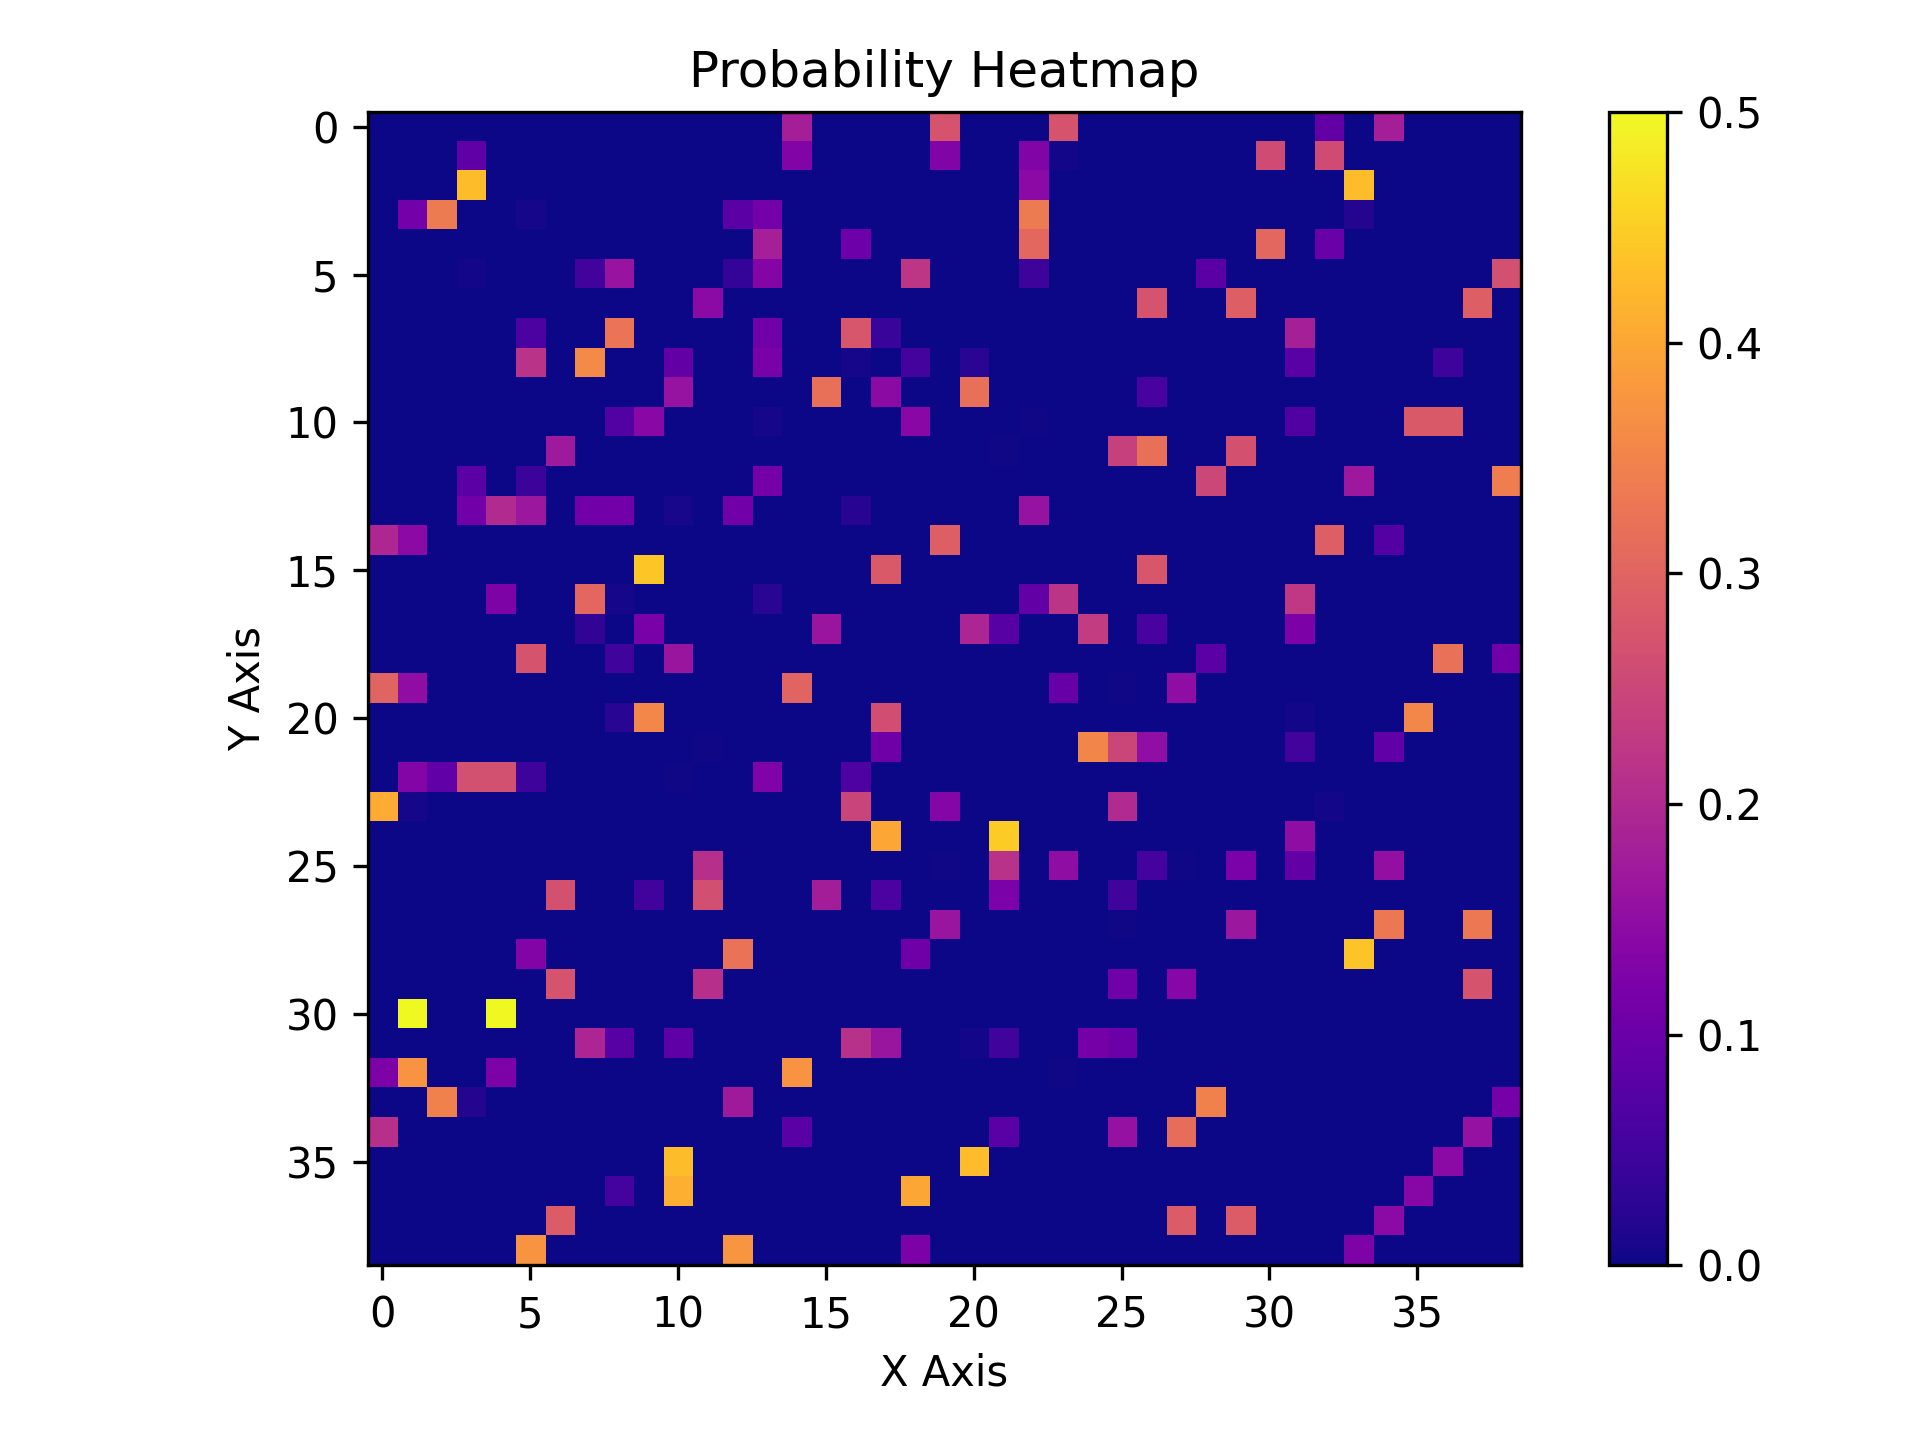
\includegraphics[width=0.4\textwidth]{fig/39-0.2-热图.png}

\caption{The probability heatmap depicts the likelihood of edges between waypoints belonging to the optimal UAV trajectory. Yellow coloration indicates higher probability of inclusion in the optimal solution.}
\label{fig:Probability Heatmap}
\end{figure}
%为此,我们首先训练了一个包含注意力机制的图卷积神经网络,利用大量具有最优解的TSP问题实例,专门针对固定规模问题生成对应的热图。然后,为了适应不同规模的问题,我们通过图采样、图转换和热图合并等技术,生成与给定悬停点集合匹配的概率热图。
To achieve this, we trained a GCN model with an integrated attention mechanism on a large dataset of TSP instances with known optimal solutions, specifically tailored for fixed-scale problem heatmap generation. To accommodate varying problem scales, we implemented graph sampling, transformation, and heatmap merging techniques to produce a probabilistic heatmap aligned with the given waypoints.
%提出的卷积神经网络模型用于求解固定规模$m$个节点问题的热图,阐述如下:
The proposed GCN model for generating heatmaps to address the fixed-size $m$ problem is described as follows:
%**输入层:** 
%输入层包含图中的节点特征和边特征。每个节点 $m_i$ 由其二维坐标 $m_i\in\left[0,1\right]^2$ 表示,这些坐标被线性映射到一个更高维度的特征空间 $\mathbb{R}^{h}$ 中。线性映射的公式为:%$$\alpha_i=A_1m_{i}+b_1$$
%其中,$A_1\in\mathbb{R}^{h\times2}$是可学习的权重矩阵,$b_1\in\mathbb{R}^h$是偏置向量。为了确保不同节点的特征在相同的尺度上,我们对 $\alpha_i$应用批归一化(Batch Normalization, BN),以减少内部协变量转移问题,提高模型的稳定性。因此,更新后的节点特征为:$$\alpha_i^{\prime}=\mathrm{BN}(\alpha_i)$$
%对于每条边 $(m_i,m_j)$,其特征 $\beta_{ij}$由两部分组成:节点间的欧几里得距离 $d_{ij}$ 和节点对间的 k-近邻关系。边特征的计算公式为:$$\beta_{ij}=A_2d_{ij}+b_2\parallel A_3\delta_{ij}^{\mathrm{k-NN}}$$
%其中,$A_{2}\in\mathbb{R}^{\frac{h}{2}\times1},A_{3}\in\mathbb{R}^{\frac{h}{2}\times3}$。$d_{ij}$被嵌入为一个$\frac h2$维的特征向量中,$\delta_{ij}^{\mathrm{k-NN}}$用于标识识节点$m_i$ 和节点$m_j$是否属于$k-$最近邻。当节点$m_i$ 和节点$m_j$属于$k-$最近邻时$\delta_{ij}^{\mathrm{k-NN}}$的值为1;如果是自连接,则值为2;否则为0。符号$\parallel$表示的是拼接操作。同样地,为了保持特征在同一尺度,我们对$\beta_{ij}$进行批归一化处理,得到:$$\beta_{ij}^{\prime}=\mathrm{BN}(\beta_{ij})$$

\textbf{Input Layer.} The input layer processes node and edge features from the graph. Each node $m_i$ is represented by its 2D coordinates $m_i\in\left[0,1\right]^2$, linearly mapped to a higher-dimensional feature space $\mathbb{R}^{h}$ through:
\begin{equation}
     \alpha_i=A_1m_{i}+b_1,
\end{equation}
where $A_1\in\mathbb{R}^{h\times2}$ is a learnable weight matrix and $b_1\in\mathbb{R}^h$ is a bias vector. To normalize node features and mitigate internal covariate shift, we apply Batch Normalization:
\begin{equation}
     \alpha_i^{\prime}=\mathrm{BN}(\alpha_i).
\end{equation}

For each edge $(m_i,m_j)$, the edge feature $\beta_{ij}$ consists of two components: the Euclidean distance $d_{ij}$ between the nodes and the $k$-nearest neighbor relationship between the node pair. The edge feature is calculated as:

\begin{equation}
    \beta_{ij}=A_2d_{ij}+b_2\parallel A_3\delta_{ij}^{\mathrm{k-NN}},
\end{equation}
where $A_{2}\in\mathbb{R}^{\frac{h}{2}\times1},A_{3}\in\mathbb{R}^{\frac{h}{2}\times3}$. The distance $d_{ij}$ embeds into a $\frac{h}{2}$-dimensional feature vector, while $\delta_{ij}^{\mathrm{k-NN}}$ encodes the $k$-nearest neighbor relationship between nodes $m_i$ and $m_j$: $\delta_{ij}^{\mathrm{k-NN}}=1$ for $k$-nearest neighbors, $\delta_{ij}^{\mathrm{k-NN}}=2$ for self-loops, and $\delta_{ij}^{\mathrm{k-NN}}=0$ otherwise. The symbol $\parallel$ denotes concatenation. To maintain consistent feature scaling, we apply batch normalization:


\begin{equation}
    \beta_{ij}^{\prime}=\mathrm{BN}(\beta_{ij}).
\end{equation}


%**卷积层:**
%在每一层的图卷积网络中,节点和边的特征会根据邻接关系进行更新。设第 $\ell$ 层的节点特征为$m_{i}^{\ell}$,特征为$e_{ij}^{\ell}$,则在第$\ell+1$层,节点特征更新为:$$\begin{array}{rcl}m_i^{\ell+1}&=&m_i^\ell+\mathrm{ReLU}\Big(\mathrm{BN}\Big(W_1^\ell m_i^\ell+\sum_{i\sim j}\eta_{ij}^\ell\odot W_2^\ell m_j^\ell\Big)\Big)\end{array}$$
%其中,注意力权重$\eta_{ij}^{\ell}=\frac{\sigma(e_{ij}^{\ell})}{\sum_{j^{\prime}\sim i}\sigma(e_{ij^{\prime}}^{\ell})+\varepsilon}$,用于控制邻居节点$m_j$对节点$i$的影响,从而实现一种自适应的聚合方式。$W_1^\ell,W_2^\ell\in\mathbb{R}^{h\times h}$是可学习的权重矩阵,ReLU 激活函数用于引入非线性。边的特征$e_{ij}^{\ell}$则结合了自身的前一层特征、起始节点$m_i$的特征$m_{i}^{\ell}$和终止节点$m_j$的特征$m_{j}^{\ell}$来更新。具体公式如下:
%$$e_{ij}^{\ell+1}\quad=\quad e_{ij}^{\ell}+\mathrm{ReLU}\Big(\mathrm{BN}\Big(W_{3}^{\ell}e_{ij}^{\ell}+W_{4}^{\ell}m_{i}^{\ell}+W_{5}^{\ell}m_{j}^{\ell}\Big)\Big)$$
%在每一层,节点和边特征通过批归一化(BN)确保稳定性,并通过残差连接保留原始特征信息:
%$$m_i^{\ell+1}=m_i^{\ell+1}+m_i^{\ell}$$
%$$\quad e_{ij}^{\ell+1}=e_{ij}^{\ell+1}+e_{ij}^{\ell}$$
\textbf{Convolutional Layer.} In each GCN layer, node and edge features are updated based on adjacency relationships. Let $m_{i}^{\ell}$ denote the node feature at layer $\ell$, and $e_{ij}^{\ell}$ the edge feature. The node features are updated as:
\begin{equation}
    \begin{array}{rcl}m_i^{\ell+1}=m_i^\ell+\mathrm{ReLU}\Big(\mathrm{BN}\Big(W_1^\ell m_i^\ell+\sum_{i\sim j}\eta_{ij}^\ell\odot W_2^\ell m_j^\ell\Big)\Big)\end{array},
\end{equation}
where the attention weight $\eta_{ij}^{\ell}$ is defined as:
\begin{equation}
    \eta_{ij}^{\ell}=\frac{\sigma(e_{ij}^{\ell})}{\sum_{j^{\prime}\sim i}\sigma(e_{ij^{\prime}}^{\ell})+\varepsilon}.
\end{equation}
This weight controls neighboring node $m_j$'s influence on node $m_i$, enabling adaptive aggregation. $W_1^\ell,W_2^\ell\in\mathbb{R}^{h\times h}$ are learnable weight matrices, and ReLU introduces non-linearity. Edge features are updated by:
\begin{equation}
    \ e_{ij}^{\ell+1}= e_{ij}^{\ell}+\mathrm{ReLU}\Big(\mathrm{BN}\Big(W_{3}^{\ell}e_{ij}^{\ell}+W_{4}^{\ell}m_{i}^{\ell}+W_{5}^{\ell}m_{j}^{\ell}\Big)\Big).
\end{equation}
Batch normalization ensures stability, while residual connections retain original feature information:
\begin{equation}
    \ m_i^{\ell+1}=m_i^{\ell+1}+m_i^{\ell},
\end{equation}
\begin{equation}
    \quad e_{ij}^{\ell+1}=e_{ij}^{\ell+1}+e_{ij}^{\ell}.
\end{equation}


%**MLP层**:
%最后一层边嵌入$e_{ij}^{\ell}$被用于计算输入图中边$(m_i,m_j)$在最短路径中的连接概率。这个概率值可以看作是路径连接的邻接矩阵上生成的概率热图。对于每条边$(m_i,m_j)$,其最短路径连接概率$p_{ij}^{\text{opt}} \in [0, 1]$由一个多层感知机(MLP)计算得到,如下所示:$$p_{ij}^{\mathrm{opt}}=\mathrm{MLP}(e_{ij}^{L})$$
\textbf{MLP Layer.} The final edge embedding $e_{ij}^{L}$ computes the connection probability of edge $(m_i, m_j)$ in the shortest path within the input graph. This probability forms the heatmap on the adjacency matrix of path connections. Each edge's shortest path probability $p_{ij}^{\text{opt}} \in [0, 1]$ is calculated via:
\begin{equation}
    \ p_{ij}^{\mathrm{opt}}=\mathrm{MLP}(e_{ij}^{L}).
\end{equation}

%**损失函数**:在训练过程中,我们给定每个TSP实例的最短路径真实排列$π$,我们将该路径转换为一个邻接矩阵,其中$\hat{p}_{ij}^{\text{opt}}$表示在最短路径中节点$m_i$和节点$m_j$之间是否存在边。如果节点$m_i$和节点$m_j$之间存在边,则$\hat{p}_{ij}^{\text{opt}} = 1$,否则$\hat{p}_{ij}^{\text{opt}} = 0$。为了优化模型,我们通过最小化加权的二元交叉熵损失(在小批次上计算平均损失)来衡量预测值与真实标签之间的误差。然而,随着问题规模的增大,负样本的比例显著增加,导致类别高度不平衡。因此,需要适当的类别权重来缓解这种影响。为此,我们计算每个TSP实例的平衡类别权重。对于负类的权重,设定为$w_0 = \frac{n^2}{(n^2 - 2n) \times c}$,对于正类的权重,设定为$w_1 = \frac{n^2}{2n \times c}$,其中$c = 2$表示类别的总数。通过这种方式计算的权重能够有效地平衡正负样本的不平衡性,从而使得模型能够更加准确地学习最短路径的特征。

\textbf{Loss Function.} During training, each TSP instance provides a ground truth shortest path permutation $\pi$, converted to an adjacency matrix where $\hat{p}_{ij}^{\text{opt}}=1$ if an edge exists between nodes $m_i$ and $m_j$, and $\hat{p}_{ij}^{\text{opt}}=0$ otherwise. We minimize the weighted binary cross-entropy loss, computed as the mean loss over mini-batches. As problem scale increases, negative samples grow significantly, causing class imbalance. To address this, we incorporate balanced class weights: for negative samples, $w_0 = {n}/{(n - 2) \times c}$; for positive samples, $w_1 = {n}/{2 \times c}$, where $c = 2$ represents the total number of classes. These weights effectively balance the positive-negative sample ratio, enabling accurate learning of shortest path features.

%一旦网络模型经过充分训练,它就能够为包含 m 个节点的问题生成热图。但是,为了适应不同规模的问题,我们应用了图采样、图转换和热图合并等技术:
Once the network model is trained, it generates heatmaps for $m$-node problems. To accommodate varying problem scales, we employ graph sampling, transformation, and sub-heatmap merging techniques.

%1)图采样:从原始图 $G$ 中提取多个包含 $m$个节点的子图$G^{'}$。每次通过选择最少被选中的节点作为聚类中心,并使用 k-近邻算法提取$m-1$个节点,直到达到设定的下界。
% \labelitemi \textbf{Graph Sampling.}
% Multiple subgraphs $G^{'}$, each containing $m$ nodes, are extracted from the original graph $G$. In each iteration, the least-selected node is chosen as the cluster center, and the $m-1$ nearest neighbors are selected using the k-nearest neighbors algorithm, until the predefined lower bound is reached.
% %2)图转换:将每个子图 $G^{'}$转换为新的图 $G^{"}$,使其节点在单位正方形内随机分布。计算子图节点的最大最小坐标,定义放大因子 $s$,并转换每个节点的坐标 $(x_i,y_i)$ 为新的坐标 $(x_i^{new},y_i^{new})$,然后将转换后的图输入训练模型生成子热图$G^{"}$。

% \labelitemi \textbf{Graph Transformation.}
% Each subgraph $G^{'}$ is transformed into a new graph $G^{"}$, with nodes randomly distributed within a unit square. The maximum and minimum coordinates of the subgraph nodes are calculated, and an amplification factor $s$ is defined. The coordinates of each node $(x_i,y_i)$ are then transformed to new coordinates $(x_i^{new},y_i^{new})$, and the transformed graph is fed into the trained model to generate the sub-heatmap $G^{"}$.
% %3)子热图合并:重复上述两个步骤,我们可以获得$I$个子热图。通过合并 $I$ 个子热图,计算每条边 $(i,j)$ 属于最短路径解的概率 $P_{ij}$,其计算公式为:$$P_{ij}=\frac{1}{O_{ij}}\times\sum_{l=1}^{I}P_{ij}^{''}(l).$$

% \labelitemi \textbf{Sub-Heatmap Merging.}
% By repeating the above two steps, we obtain $I$ sub-heatmaps. The probability $P_{ij}$ that each edge $(i,j)$ belongs to the shortest path solution is computed by aggregating the results from the $I$ sub-heatmaps, as follows:
% \begin{equation}
%      P_{ij}=\frac{1}{O_{ij}}\times\sum_{l=1}^{I}P_{ij}^{''}(l).
% \end{equation}
% %其中 $P_{ij}^{''}(l)$ 是在第 $l$ 个子热图$G^{"}$中的最优解概率。最后,去除 $P_{ij}<{1}0^{-4}$ 的边,以减少后续搜索空间。
% Here, $P_{ij}^{''}(l)$ represents the optimal solution probability for edge $(i,j)$ in the $l$-th sub-heatmap $G^{"}$. Finally, edges with $P_{ij}<{1}0^{-4}$ are removed to reduce the search space for subsequent steps.
\paragraph{Step 1: Graph Sampling.} Multiple $m$-node subgraphs $G'$ are extracted from the original graph $G$. During each iteration, the least-selected node $c$ (with minimum selection count $O_c$) serves as the cluster center, and its $m-1$ nearest neighbors are selected using the $k$-NN algorithm. This process continues until all nodes reach a predefined selection threshold, ensuring balanced coverage of the original graph.

\paragraph{Step 2: Graph Transformation.} Each subgraph $G'$ is transformed into $G''$ with nodes mapped to a unit square. After calculating the bounding box coordinates $(x^{min}, x^{max}, y^{min}, y^{max})$, an amplification factor $s = 1/\max(x^{max}-x^{min}, y^{max}-y^{min})$ transforms each node from $(x_i,y_i)$ to $(x_i^{new},y_i^{new})=(s \times (x_i - x^{min}), s \times (y_i - y^{min}))$. Each transformed graph is then processed by our trained model to generate a corresponding sub-heatmap.

\paragraph{Step 3: Sub-Heatmap Merging.} By repeating the above steps, we obtain $I$ sub-heatmaps collected in set $L_h$. The probability $P_{ij}$ of edge $(i,j)$ belonging to the shortest path is computed by:
\begin{equation}
     P_{ij}=\frac{1}{O_{ij}}\times\sum_{l=1}^{I}P_{ij}^{''}(l),
\end{equation}
where $P_{ij}^{''}(l)$ represents the optimal solution probability for edge $(i,j)$ in the $l$-th sub-heatmap and $O_{ij}$ tracks the number of times edge $(i,j)$ appears across all subgraphs. Edges with $P_{ij}<10^{-4}$ are removed to reduce the search space.


%%%%%%%%%热图生成伪代码
% \algrenewcommand{\algorithmicrequire}{\textbf{Input:}}  % 修改 Input 关键字
% \algrenewcommand{\algorithmicensure}{\textbf{Output:}}  % 修改 Output 关键字
% \begin{algorithm}
% \caption{Heatmap Generation Algorithm}
% \begin{algorithmic}[1]
% \Require Graph $G$, trained model.
% \Ensure Heatmap $H$
% \State Initialize: $O_i = 0$ for all nodes, $O_{ij} = 0$ for all edges, $L_s$ ;
% \While{$\min(O_i) < threshold$} 
%     \State Select node $c$ with minimum $O_c$ ;
%     \State Use $k$-NN to select $m-1$ nodes around $c$ forming subgraph $G'$ ;
%     \State Increment $O_i$, $O_{ij}$ for nodes and edges in $G'$ ;
%     \State Add $G'$ to $L_s$ ;
% \EndWhile 

% \For{each subgraph $G'$ in $L_s$} 
%     \State Compute $x^{min}, x^{max}, y^{min}, y^{max}$ for $G'$ ;
%     \State $s = 1 / \max(x^{max} - x^{min}, y^{max} - y^{min})$ ;
%     \For{each node $(x_i, y_i)$ in $G'$} 
%         \State $(x_i^{new}, y_i^{new}) = (s \times (x_i - x^{min}), s \times (y_i - y^{min}))$ ;

%     \EndFor 
    
%     \State Add transformed graph $G''$ to $L_t$ ;
    
% \EndFor 

% \State Initialize $L_h$ ;
% \For{each transformed graph $G''$ in $L_t$} 
%     \State Generate sub-heatmap $H''$ using model ;
%     \State Append $H''$ to $L_h$ ;
% \EndFor 
% \State Initialize final heatmap $H$ with zeros ;
% \For{each edge $(i, j)$ in $G$} 
%     \State $P_{ij} = \frac{1}{O_{ij}} \sum_{l=1}^{I} P''_{ij}(l)$ ;
%     \State Update $H$ with $P_{ij}$ for edge $(i, j)$ ;
%     \If{$P_{ij} < 1e-4$} 
%         \State Remove edge $(i, j)$ from $H$ ;
%     \EndIf  
% \EndFor 
% \State \Return Heatmap $H$

% \end{algorithmic}
% \end{algorithm} 

%%%%%%%%%热图生成伪代码
% \algrenewcommand{\algorithmicrequire}{\textbf{Input:}}
% \algrenewcommand{\algorithmicensure}{\textbf{Output:}}
% \begin{algorithm}
% \caption{Heatmap Generation Algorithm}
% \begin{algorithmic}[1]
% \Require Graph $G$, trained model
% \Ensure Heatmap $H$
% \State Initialize: $O_i = 0$ for all nodes, $O_{ij} = 0$ for all edges, $L_s = \emptyset$
% \While{$\min(O_i) < \text{threshold}$} 
%     \State Select node $c$ with minimum $O_c$
%     \State Use $k$-NN to select $m-1$ nodes around $c$ to form subgraph $G'$
%     \State Increment $O_i$, $O_{ij}$ for nodes and edges in $G'$
%     \State Add $G'$ to $L_s$
% \EndWhile 

% \State Initialize $L_t = \emptyset$
% \For{each subgraph $G' \in L_s$} 
%     \State Compute bounding box: $x^{\min}, x^{\max}, y^{\min}, y^{\max}$ for $G'$
%     \State $s \gets 1 / \max(x^{\max} - x^{\min}, y^{\max} - y^{\min})$
%     \For{each node $(x_i, y_i) \in G'$} 
%         \State $(x_i^{\text{new}}, y_i^{\text{new}}) \gets (s \times (x_i - x^{\min}), s \times (y_i - y^{\min}))$
%     \EndFor 
%     \State Add transformed graph $G''$ to $L_t$
% \EndFor 

% \State Initialize $L_h = \emptyset$
% \For{each transformed graph $G'' \in L_t$} 
%     \State Generate sub-heatmap $H''$ using trained model
%     \State Append $H''$ to $L_h$
% \EndFor 

% \State Initialize final heatmap $H$ with zeros
% \For{each edge $(i, j) \in G$} 
%     \State $P_{ij} \gets \frac{1}{O_{ij}} \sum_{l=1}^{|L_h|} P_{ij}''(l)$
%     \State Update $H$ with $P_{ij}$ for edge $(i, j)$
%     \If{$P_{ij} < 10^{-4}$} 
%         \State Remove edge $(i, j)$ from $H$
%     \EndIf 
% \EndFor 
% \State \Return Heatmap $H$
% \end{algorithmic}
% \end{algorithm}




\subsubsection{Reinforcement Learning based Trajectory Optimization }

%UTICA:	heatmap-gUided reinforcemenT learnIng trajeCtory optimizAtion

%%基于上述生成的悬停点集合对应的热图,我们采用一种由强化学习驱动的路径搜索方法来寻找无人机遍历悬停点最优的遍历顺序。这个搜索过程被建模为一个马尔可夫决策过程(MDP),其中从初始状态$\pi$出发,逐步应用动作$a$,以不断优化并达到新的目标状态$\pi^{*}$。其相关函数设计如下:
To optimize the UAV's traversal sequence, we utilize a reinforcement learning-driven path search method that leverages the heatmap corresponding to the generated set of waypoints. This search process is modeled as a Markov Decision Process (MDP), where actions $\boldsymbol{a}$ are applied iteratively starting from an initial state $\boldsymbol{\pi}$, gradually optimizing the path until a target state $\boldsymbol{\pi^{*}}$ is reached. The relevant function designs are described as follows:

%%状态函数:状态函数定义了无人机遍历所有悬停点的一个完整解,即所有悬停点的排列$\pi = (\pi_{1},\pi_{2},\ldots,\pi_{n})$。每个状态代表了无人机的一个潜在的路径,从起点开始,遍历每一个悬停点,并最终返回起点。

\textbf{State Function.} The state function defines a complete solution for the UAV traversal sequence across all waypoints, represented as a permutation of waypoints $\boldsymbol{\pi} = (\pi_{1},\pi_{2},\ldots,\pi_{n})$. Each state represents a potential UAV path that starts at the initial point, traverses each waypoint exactly once, and returns to the starting point.

%%动作函数:动作函数定义了从一个状态$π$到另一个状态$π^{*}$的转换。在无人机飞行路径规划中,一个动作可以被视为一个$k\mathrm{-opt} (2\leq k\leq n)$变换,它首先删除$k$条边(例如,$(a_i,b_i),1\leq i\leq k$),然后添加$k$条边(例如,$(b_i,a_{i+1}),1\leq i\leq k$)来形成一个新的路径。动作$a$可以表示为$\boldsymbol{a}=(a_{1},b_{1},a_{2},b_{2},\ldots,a_{k},b_{k},a_{k+1})$,其中k是变量,并且起点和与终点必须相同,即$a_{k+1} = a_{1}$。例如,现在有一个遍历顺序$A->B->C->D->E->F->A$,其中$a_1$对应$C$,$b_1$对应$B$,$a_2$对应$E$,$b_2$对应$F$,$a_3$对应$C$。动作$a$就可以表示为$\boldsymbol{a}=(a_{1},b_{1},a_{2},b_{2},a_{3})$,其含义是删除边BC和EF,并添加新的边BE和FC。应用该动作后,新的遍历顺序为$A->B->E->D->C->F->A$。

\textbf{Action Function.} 
The action function transforms one state $\boldsymbol{\pi}$ to another state $\boldsymbol{\pi^{*}}$. In UAV trajectory optimization, an action represents a $k\mathrm{-opt}$ operation ($2 \leq k \leq n$) that replaces $k$ edges with $k$ new edges to form a different path. An action $\boldsymbol{a}$ is denoted as $\boldsymbol{a}=(a_{1},b_{1},a_{2},b_{2},\ldots,a_{k},b_{k},a_{k+1})$, where $a_{k+1} = a_{1}$ ensures the path remains closed. %For example, given path \( A \to B \to C \to D \to E \to F \to A \), the action \(\boldsymbol{a} = (C, B, E, F, C) \) removes edges \( BC \) and \( EF \), adds edges \( BE \) and \( FC \), resulting in path \( A \to B \to E \to D \to C \to F \to A \).



While these $k$-opt operations provide a mechanism for path modification, efficiently navigating the vast solution space remains challenging, particularly as $k$ increases. The key challenge lies in selecting which edges to replace among the exponential number of possibilities. To address this, we develop a learning-based approach that intelligently samples promising actions according to historical performance. Algorithm 2 presents an integrated framework that combines local neighborhood search with Monte Carlo Tree Search (MCTS) for efficient exploration of the solution space.

%%首先,我们随机选择一个起始节点 $\pi_1$,然后依次选择未访问的节点,并按照与 $\exp(P_{\pi_{i}j})$ 成正比的概率选择每个候选节点,直到形成完整的遍历顺序$\pi = (\pi_1, \pi_2, \ldots, \pi_n)$。在初始状态下,首先使用简单方法在小邻域内进行搜索,应用第一个改进动作,直到没有 $k=2$ 的改进动作。若无改进,扩展邻域并使用 $k>2$ 的动作,但这可能会包含大量动作。由于直接枚举不可行,我们采用蒙特卡洛树搜索(MCTS)方法,迭代采样有潜力的动作,并选择能够改善当前状态的动作。其详细过程如下


Algorithm 2 begins by initializing weight matrix $W$ from heatmap probabilities and visit matrix $Q$ to track edge selection frequency. An initial solution is generated by sequentially selecting nodes with probabilities proportional to $\exp(P_{\pi_{i j}})$. The optimization process then alternates between two phases: a simple 2-opt neighborhood search for local improvements, and an MCTS-based exploration when local optima are encountered.





In the MCTS phase, actions are constructed incrementally through probabilistic node selection. For each step, the algorithm computes a potential value $Z_{b_{i j}}$ that balances exploitation of high-weight edges with exploration of less-visited options:
\begin{equation}
    Z_{b_{i j}} = \frac{W_{b_{i j}}}{\Omega_{b_i}} + \alpha\sqrt{\frac{\ln(M+1)}{Q_{b_{i j}}+1}},
\end{equation}
where $\Omega_{b_i}$ represents the average edge weight from node $b_i$. Candidate nodes form set $X$ where $W_{b_{i j}} \geq 1$, excluding already connected nodes. Selection probabilities are computed as:
\begin{equation}
    P_{j} = \frac{Z_{b_{i j}}}{\sum_{l \in X} Z_{b_i l}}.
\end{equation}

When an improving action is found, the algorithm updates edge weights proportionally to the improvement quality:
\begin{equation}
    W_{b_i a_{i+1}} \gets W_{b_i a_{i+1}} + \beta\left[\exp\left(\frac{L(\boldsymbol{\pi}) - L(\boldsymbol{\pi^{new}})}{L(\boldsymbol{\pi})}\right) - 1\right].
\end{equation}
This adaptive learning mechanism progressively biases the search toward promising solution regions while maintaining sufficient exploration through the UCB term in the potential function. The visit matrix $Q$ tracks edge selection frequency, ensuring balanced exploration of the search space over time.

\algrenewcommand{\algorithmicrequire}{\textbf{Input:}}
\algrenewcommand{\algorithmicensure}{\textbf{Output:}}
\begin{algorithm}
\caption{UTICA: Heatmap-Guided Reinforcement Learning Trajectory Optimization}
\begin{algorithmic}[1]
\Require Heatmap $P$, time limit $T$, parameters $\alpha$, $\beta$
\Ensure Optimal traversal path $\boldsymbol{\pi^*}$
\State Initialize: $W_{ij} = 100 \times P_{ij}$, $Q_{ij} = 0$ for all $i,j$, $M = 0$
\State Generate initial path $\boldsymbol{\pi}$ with probability $\propto \exp(P_{\pi_{i j}})$
\State $\boldsymbol{\pi^*} \gets \boldsymbol{\pi}$

\While{time $< T$}
    \State Apply first-improvement $k=2$ actions until no further improvement
    \If{no improvement found}
        % \State // MCTS phase
        \State Randomly select $a_1$, determine $b_1$, and initialize $\boldsymbol{a}$
        \State $i \gets 1$
        \While{$a_{i+1} \neq a_1$}
            \State Calculate $\Omega_{b_i}$ as average of $W_{b_{i j}}$ across all edges 
            \State Compute $Z_{b_{i j}}$ for all candidate nodes
            \State Identify set $X$ where $W_{b_{i j}} \geq 1$ 

            \State Select $a_{i+1}$ with probability $P_j$
            \State Determine $b_{i+1}$ and append $(a_{i+1}, b_{i+1})$ to $\boldsymbol{a}$

            \State $i \gets i + 1$
            \If{$a_{i+1} = a_1$}
                \State Break
            \EndIf
        \EndWhile
        
        \State $\boldsymbol{\pi^{new}} \gets \text{ApplyAction}(\boldsymbol{\pi}, \boldsymbol{a})$
        \If{$L(\boldsymbol{\pi^{new}}) < L(\boldsymbol{\pi})$}
            \State $\boldsymbol{\pi} \gets \boldsymbol{\pi^{new}}$
            \For{each edge $(b_i, a_{i+1})$ in $\boldsymbol{a}$}
                \State $W_{b_i a_{i+1}} \gets W_{b_i a_{i+1}} + \beta[\exp(\frac{L(\boldsymbol{\pi}) - L(\boldsymbol{\pi^{new}})}{L(\boldsymbol{\pi})}) - 1]$
            \EndFor
            \If{$L(\boldsymbol{\pi}) < L(\boldsymbol{\pi^*})$}
                \State $\boldsymbol{\pi^*} \gets \boldsymbol{\pi}$
            \EndIf
        \Else
            \State Randomly reset $\boldsymbol{\pi}$ to a new starting state
        \EndIf
    \EndIf
    \State Update $M$ and $Q_{b_i a_{i+1}}$ for all edges in $\boldsymbol{a}$
\EndWhile
\State \Return $\boldsymbol{\pi^*}$
\end{algorithmic}
\end{algorithm}

The UTICA algorithm operates in two phases with distinct computational requirements. For heatmap generation, the Graph Convolutional Network processes each subgraph with time complexity $O(m^2)$ where $m$ is the fixed-size problem scale, resulting in overall complexity $O(|L_s| \cdot m^2)$ for $|L_s|$ sampled subgraphs. The reinforcement learning phase operates within the time limit $T$, with each iteration requiring $O(K)$ operations for $K$ waypoints. The space complexity is dominated by the weight matrix $W$ and visit matrix $Q$, requiring $O(K^2)$ storage. This computational efficiency makes UTICA practical for UAV trajectory planning applications.




\section{EXPERIMENTS}
\subsection{Experimental Setup}
%我们考虑一个1公里×1公里的地面网络大小。网络中传感器的数量从100到500不等,随机的分布在该区域中。我们采用Intel Berkeley Research Lab中,54个传感器38天的真实传感数据,来确定相邻传感器节点之间的空间数据相似度$c(i,j)$的分布律。以此来模拟我们实验中相邻传感器节点的空间数据相似度$c(i,j)$的数值。并且,对于任意两个相邻的传感器节点$v_i$, $v_j$,其空间数据相似度$c(i,j)$的值从区间$[0,C_{max}]$中随机选择的,其中$C_{max}$的值为1。这意味着,任意两个相邻的传感器之间的空间数据相关性是一个介于0到1之间的随机数,当这个值越靠近1的时,表示两个传感器的数据高度相关;而当这个值接近0时,则表示两个传感器的数据几乎不相关。
Our simulation employs a 1 km $\times$ 1 km ground network with 100-500 randomly distributed IoT devices. The communication range between devices is set to $r_{com}=100$ meters. The spatial data similarity values $c(i,j)$ between neighboring devices are based on real sensor data collected from 54 sensors over 38 days at the Intel Berkeley Research Lab \cite{14-IntelBerkeley2013}. For any adjacent devices $v_i$ and $v_j$, we assign a random similarity value $c(i,j)$ from the interval $[0, 1]$, where values approaching 1 indicate high data correlation and values near 0 represent low correlation. This approach allows us to realistically model the spatial relationships between IoT devices in our experimental scenarios.


%此外,我们通过一个具有NVIDIA GeForce RTX 3090 的WSL子系统上使用Pytorch 1.0.1.post2和Python 3.7来实现所提出的网络模型,并由Adam优化器训练,初始学习率为0.001,每5个训练周期在10000个实例的验证集上评估模型,如果验证损失没有比之前的损失至少降低1%,则将学习率除以1.01进行衰减。为了训练模型,我们生成了990,000个具有20个节点的具有最优路径的实例作为训练集,使用精确求解器Concorde产生的解决方案作为基准。
We implemented our model using PyTorch 1.0.1.post2 and Python 3.7 on a WSL subsystem with an NVIDIA GeForce RTX 3090 GPU. Training utilized the Adam optimizer with an initial learning rate of 0.001, which was decayed by a factor of 1.01 whenever the validation loss failed to decrease by at least 1\% after 5 epochs. The model was evaluated every 5 epochs on a validation set of 10,000 instances. For training, we generated 990,000 instances containing 20 nodes each, with optimal paths determined by the Concorde exact solver as benchmarks.


\subsection{Baselines and Metrics}
%我们在相同的仿真设置下,将所提出的算法与三种基准算法以及文献[learning+greedy]中的算法Learning+Greedy进行了比较。
%- 遗传算法:是一种流行的启发式算法,模拟了自然界中动物的繁殖过程。它包括交叉、变异和选择等几个部分。其主要的思想是在每次的迭代中生成大量的可行解,并在其中搜索最佳解。
%- 自组织映射:自组织映射是一种无监督学习算法,通过将路径优化问题的决策空间映射到低维网格结构中,利用竞争学习机制找到最优路径。
%- 蚁群算法:蚁群算法是一种基于蚂蚁行为的优化方法,通过信息素的积累和蒸发引导多个蚂蚁选择最佳路径。
%- Learning+Greedy:该方法通过图神经网络生成概率图,并结合贪心搜索算法优化路径规划。该方法通过为每个节点分配概率,并在路径搜索中选择概率最高的边来逐步构建最优路径。
Under identical simulation conditions, we benchmark the proposed algorithm against four baseline methods.


\begin{itemize}
    \item \textbf{Genetic Algorithm} \cite{16-GA}: A metaheuristic that mimics natural selection by generating multiple feasible solutions and evolving them through crossover, mutation, and selection operations to progressively approach the optimal solution.

    \item \textbf{Self-Organizing Map} \cite{17-SOM}: An unsupervised learning algorithm that maps the path optimization problem onto a low-dimensional grid structure, using competitive learning mechanisms to identify optimal trajectories.

    \item \textbf{Ant Colony Optimization} \cite{18-ACO}: A nature-inspired method based on ant foraging behavior, where multiple agents construct solutions while depositing and following pheromone trails to collectively identify efficient paths.

    \item \textbf{Learning+Greedy} \cite{15-learning+greedy}: A hybrid approach that leverages a graph neural network to generate a probability graph, then employs greedy search to sequentially select highest-probability edges when constructing paths.

\end{itemize}


\subsection{Experimental Results}
%为了验证不同方法的可扩展性,我们选择了100到500的无线传感器网络规模。
% 本节评估了参数 $C_{max}$ 对冗余数据量、总能耗以及悬停点数量的影响。如图[Fig.3.a]所示,我们分析了 $C_{max}$ 与冗余数据量之间的关系。实验结果表明,在不同的 $C_{max}$ 值下,所提出的方法对网络中冗余数据的抑制效果有所差异。具体而言,当网络规模较小时,由于传感器节点分布较为分散,$C_{max}$ 对冗余数据抑制的影响较为有限;随着网络规模增大,传感器节点逐渐集中,$C_{max}$ 对冗余数据抑制的效果逐渐增强。此外,在相同网络规模下,较大的 $C_{max}$ 值能够更有效地减少冗余数据量,从而降低无人机在数据采集过程中所收集的冗余数据。

% 图[Fig.3.b]进一步展示了 $C_{max}$ 对总能耗和悬停点数量的影响,分别考虑了网络规模为100、300和500节点的情况。结果表明,随着 $C_{max}$ 的增大,网络抑制冗余数据的能力显著提升,进而导致总能耗的减少。同时,图中还显示了不同 $C_{max}$ 值下无人机悬停点数量的变化。随着网络规模的增大,无人机悬停点的数量呈上升趋势。

% 此外,与其他路径规划方法的比较进一步验证了我们方法的有效性如图[Fig.3.c]所示。在网络规模为500且 $C_{max}=1$ 的情况下,我们提出的路径规划算法始终能实现最短的飞行距离,优于其他路径规划算法。例如,与GA相比,我们的方法缩短了约12.05%的飞行距离;与Learning+Greedy算法相比,减少了约11.41%;与SOM算法相比,缩短了约7.09%;与ACO算法相比,减少了约11.69%。这些结果表明,在优化飞行距离方面,所提出的路径规划算法具有明显优势,尤其在大规模网络下,能够有效缩短飞行距离并提高整体效率。

To evaluate the scalability of different approaches, we consider wireless sensor network sizes ranging from 100 to 500 nodes.
\subsubsection{Comparative Analysis for $C_{max}$}


\begin{figure*}[htbp]
	\centering
	\subfloat[Impact on suppressing redundant data volume.]{
		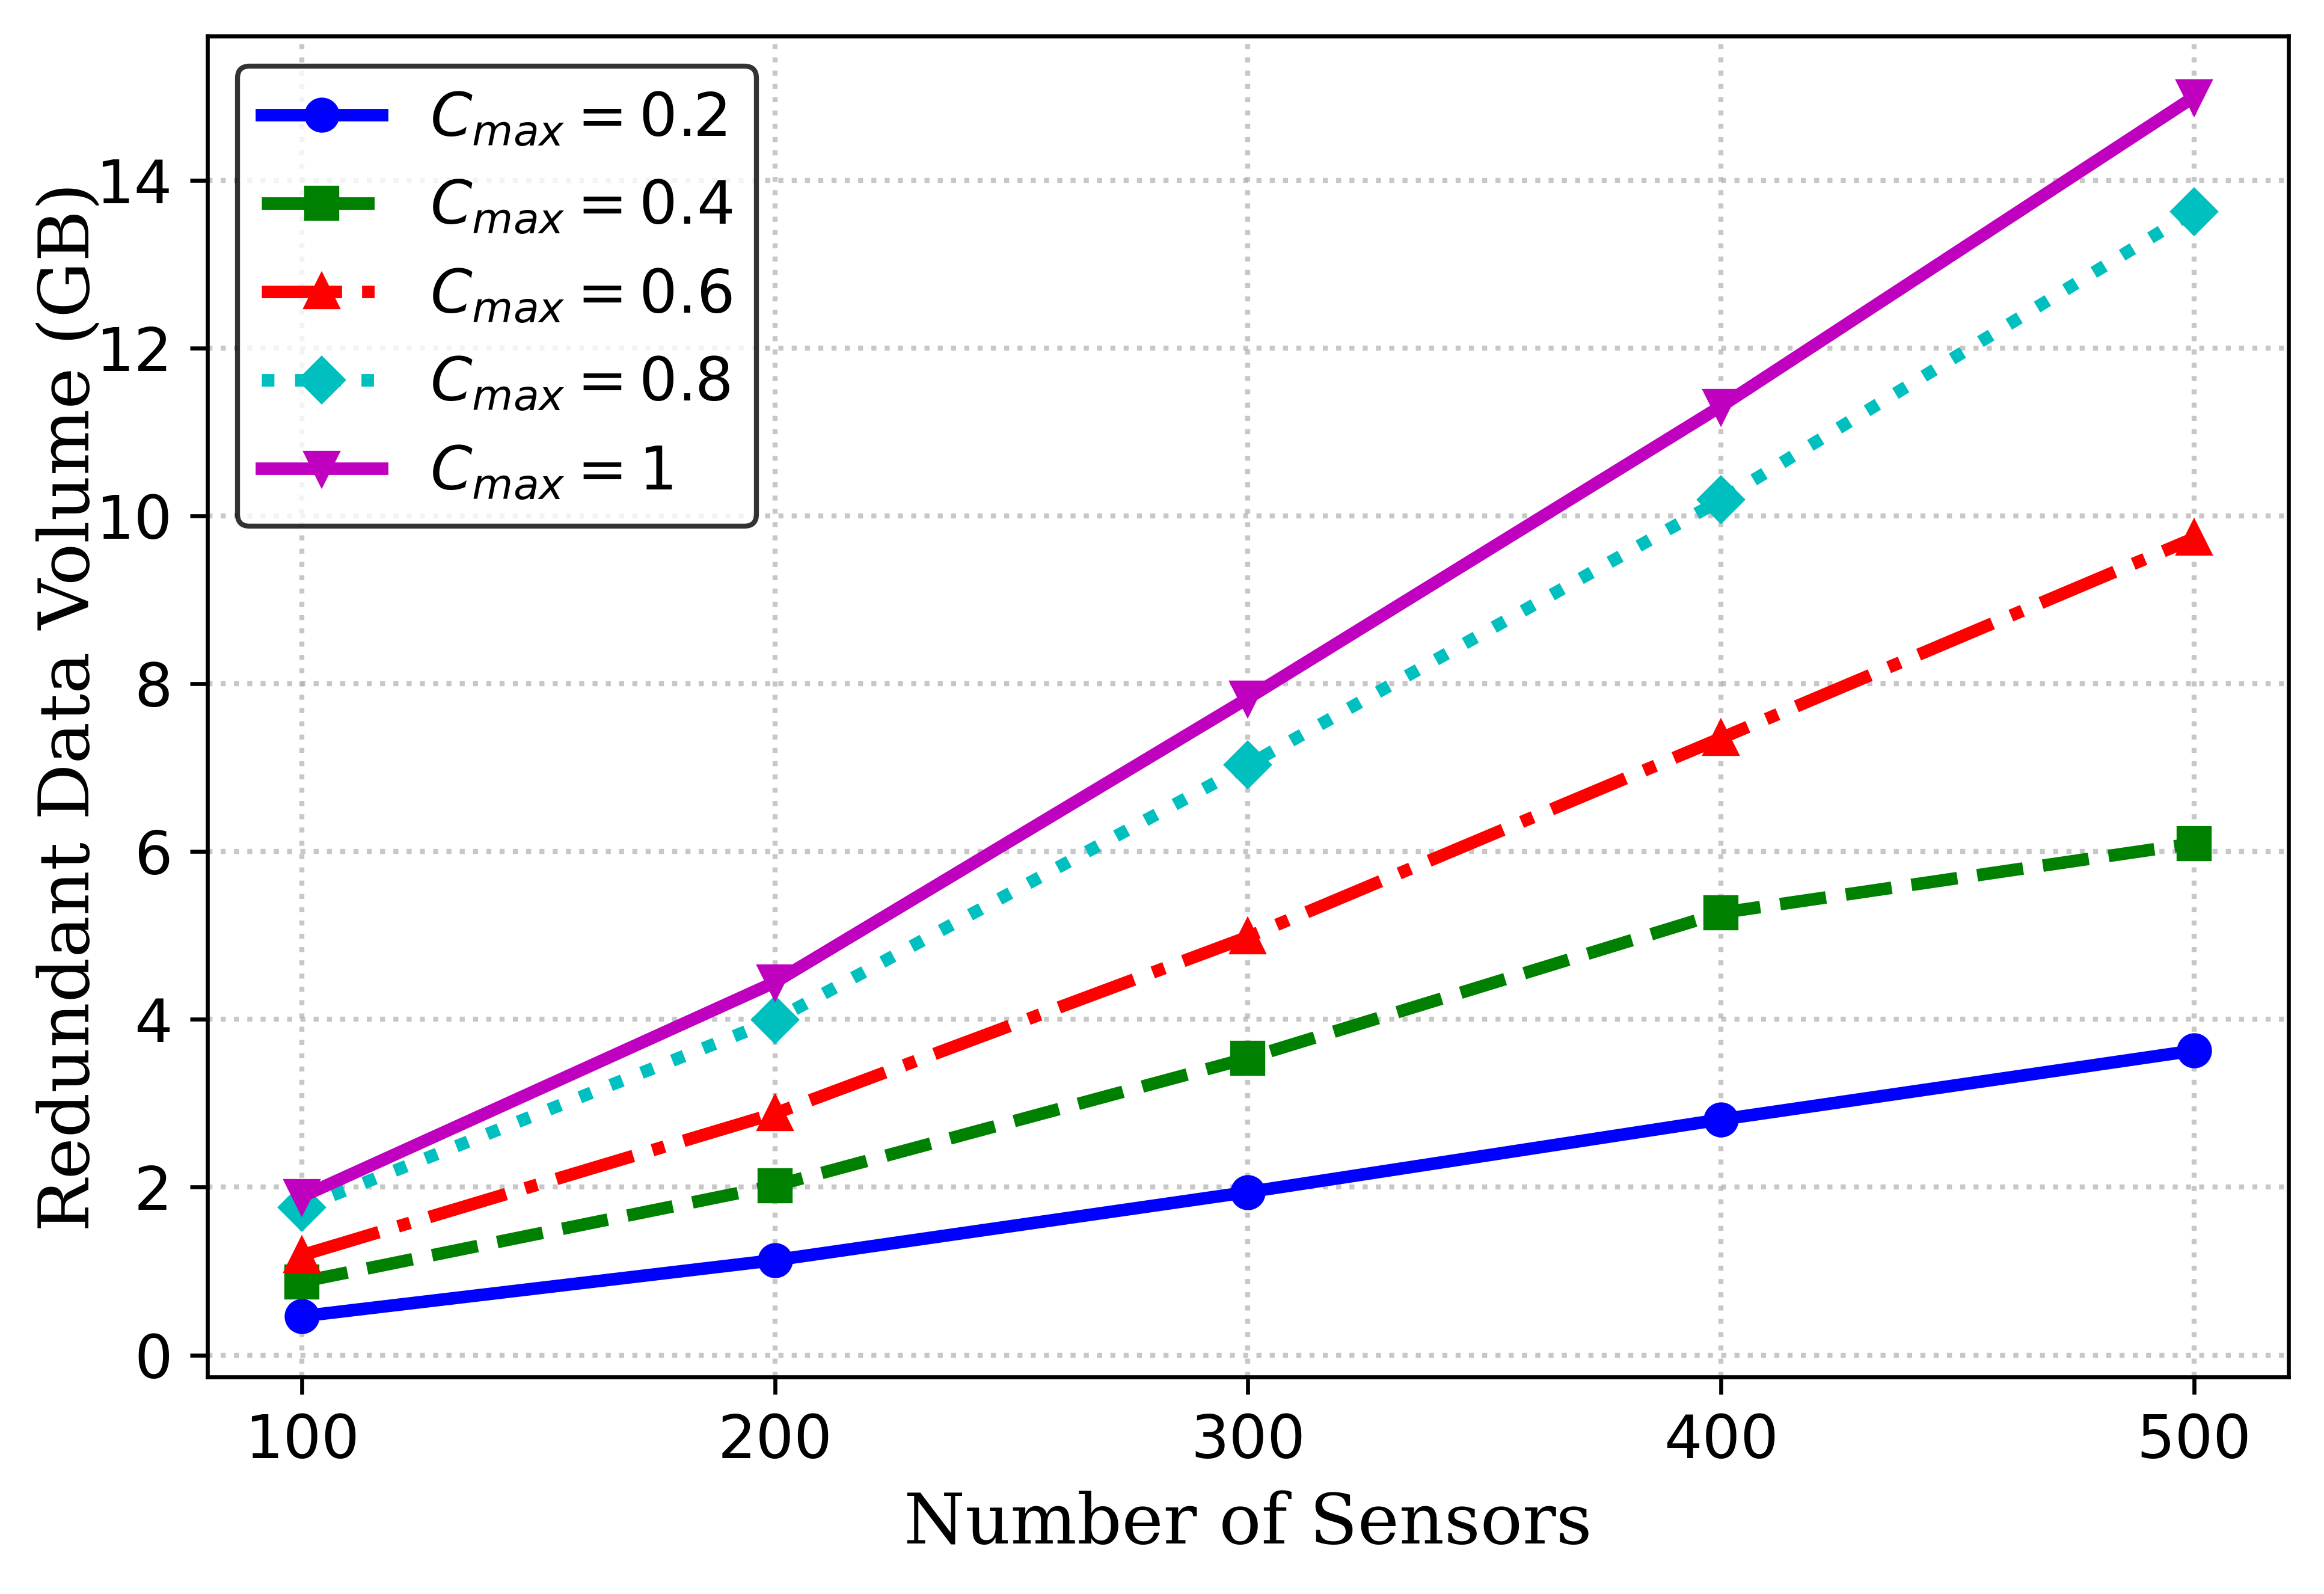
\includegraphics[width=0.3\linewidth]{fig/Different_Cmax_IEEE.png}
		\label{chutian1}
	}
	\hfill
	\subfloat[Impact on Energy Consumption and waypoints.]{
		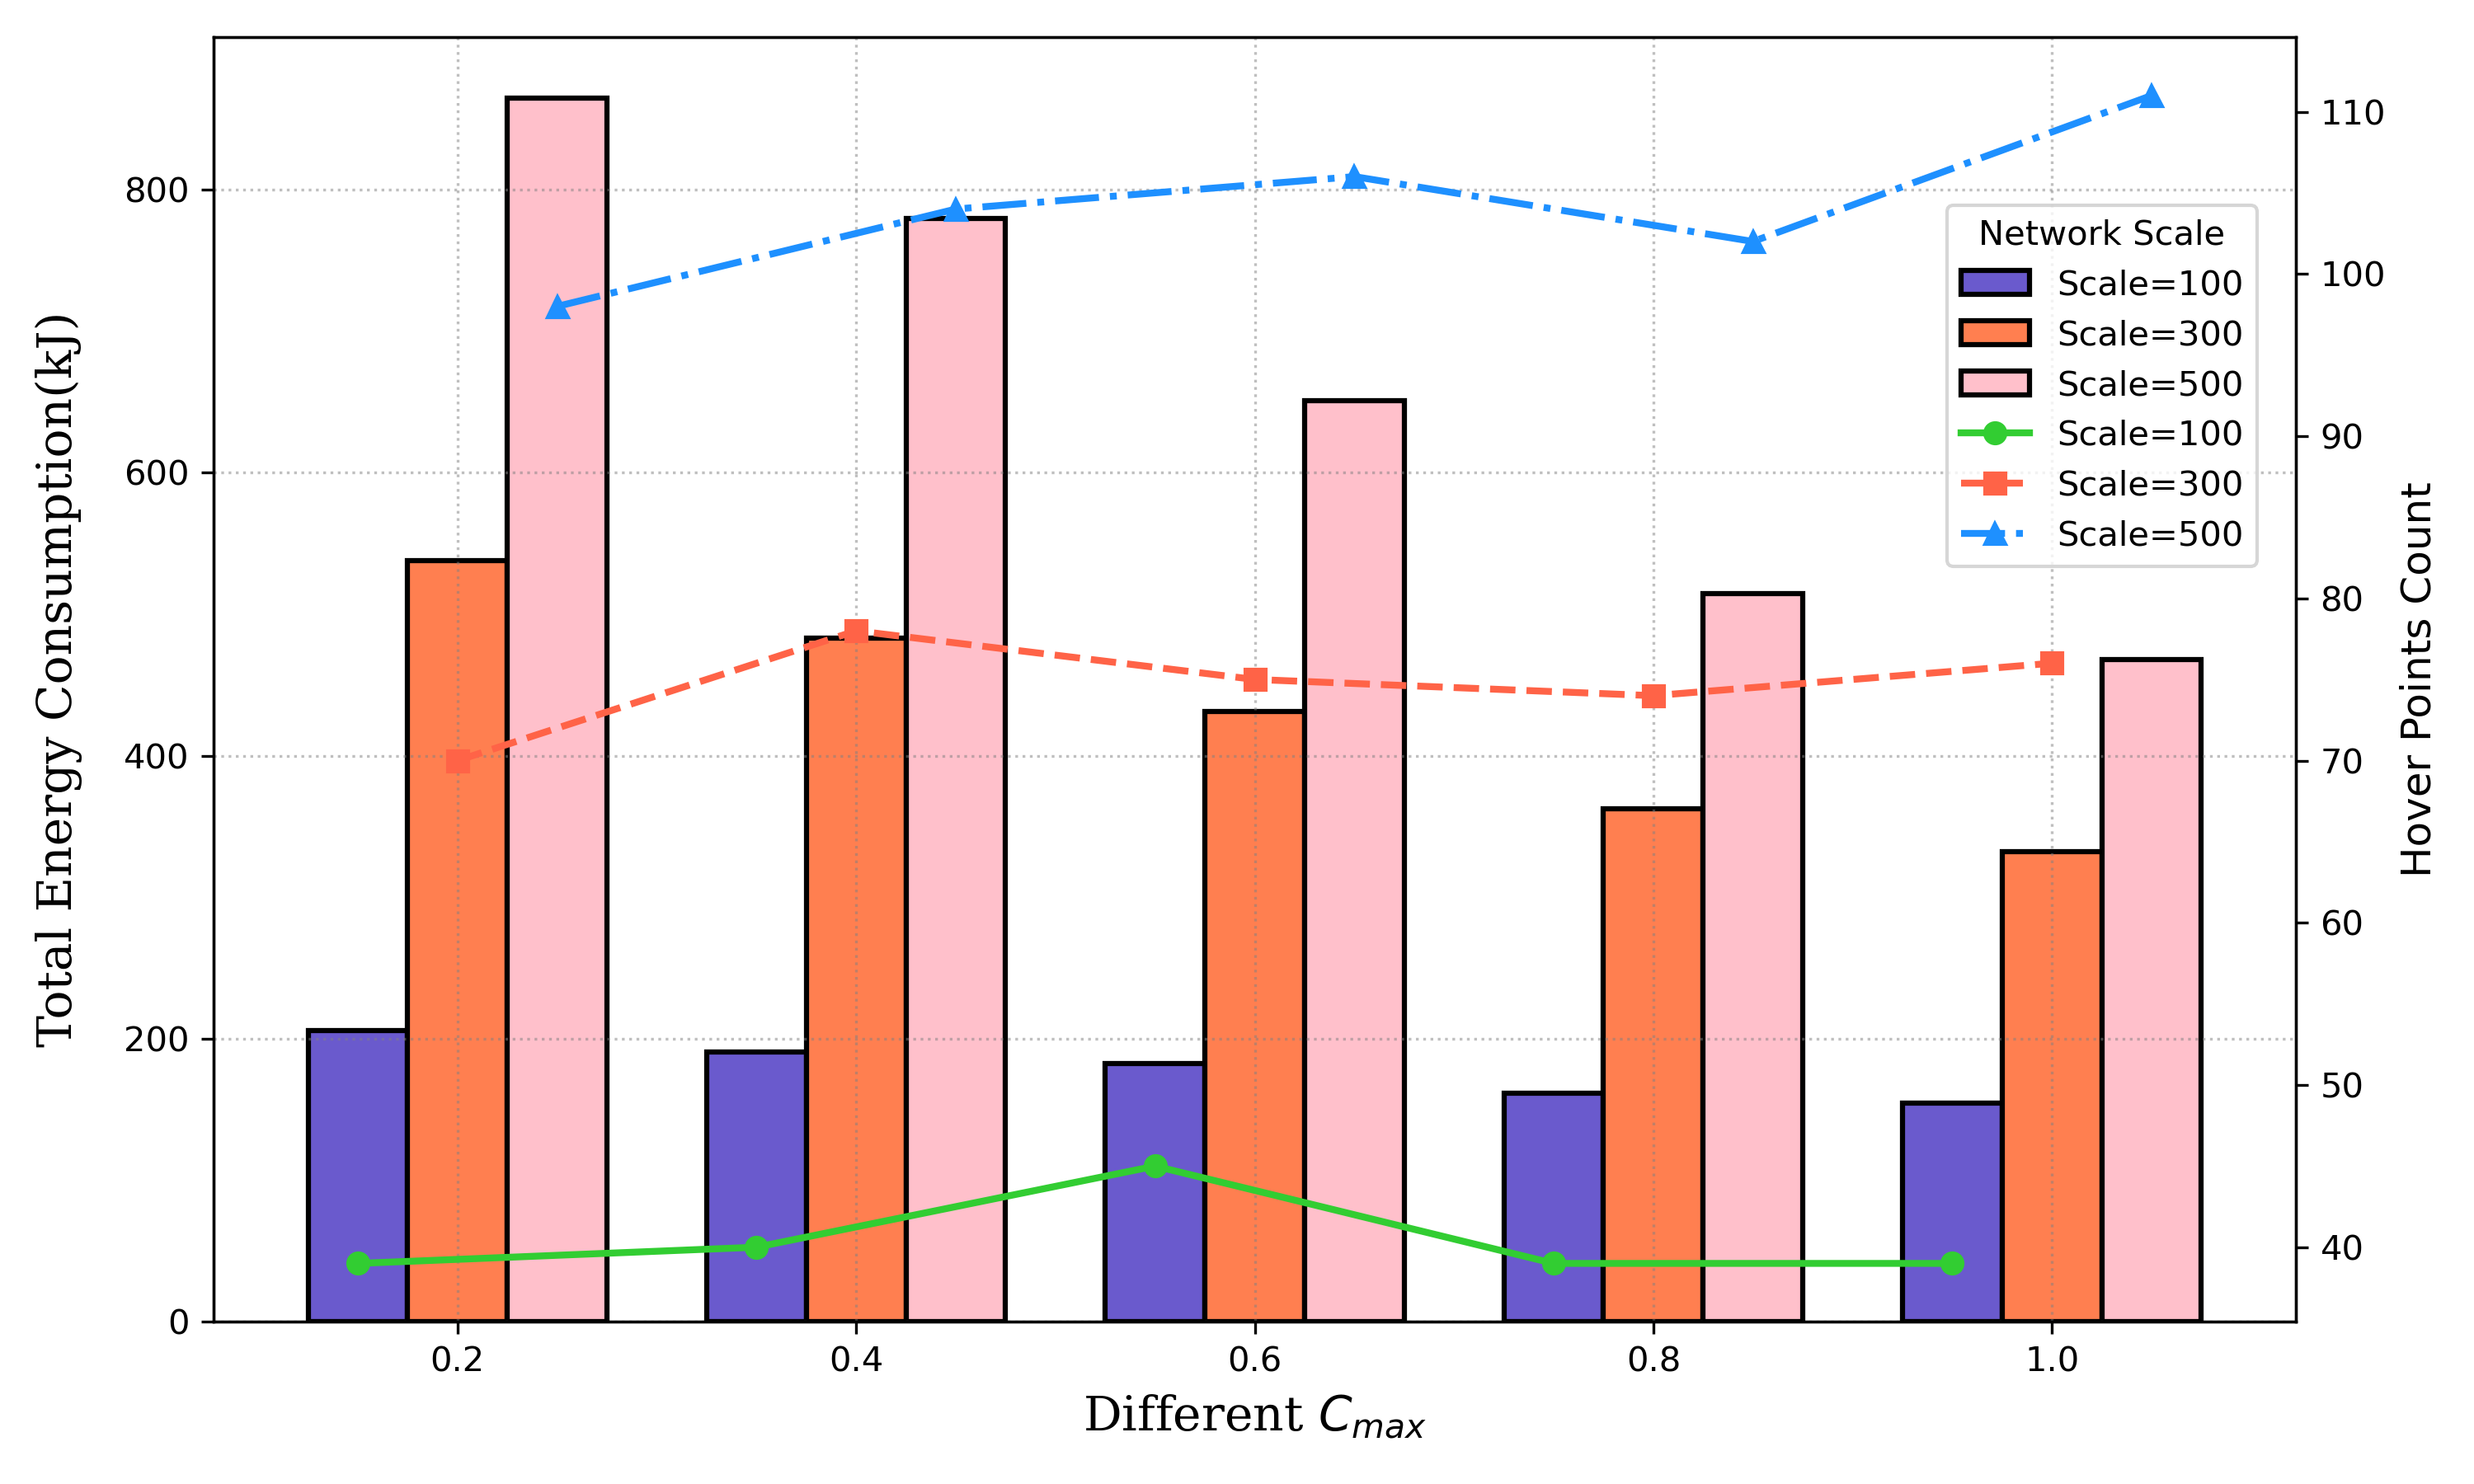
\includegraphics[height=3.7cm]{fig/Different_Cmax_Scale_modified.png}  % 仅调整此图的高度
		\label{chutian2}
	}
	\hfill
	\subfloat[Impact of different $C_{max}$ on flight distance.]{
		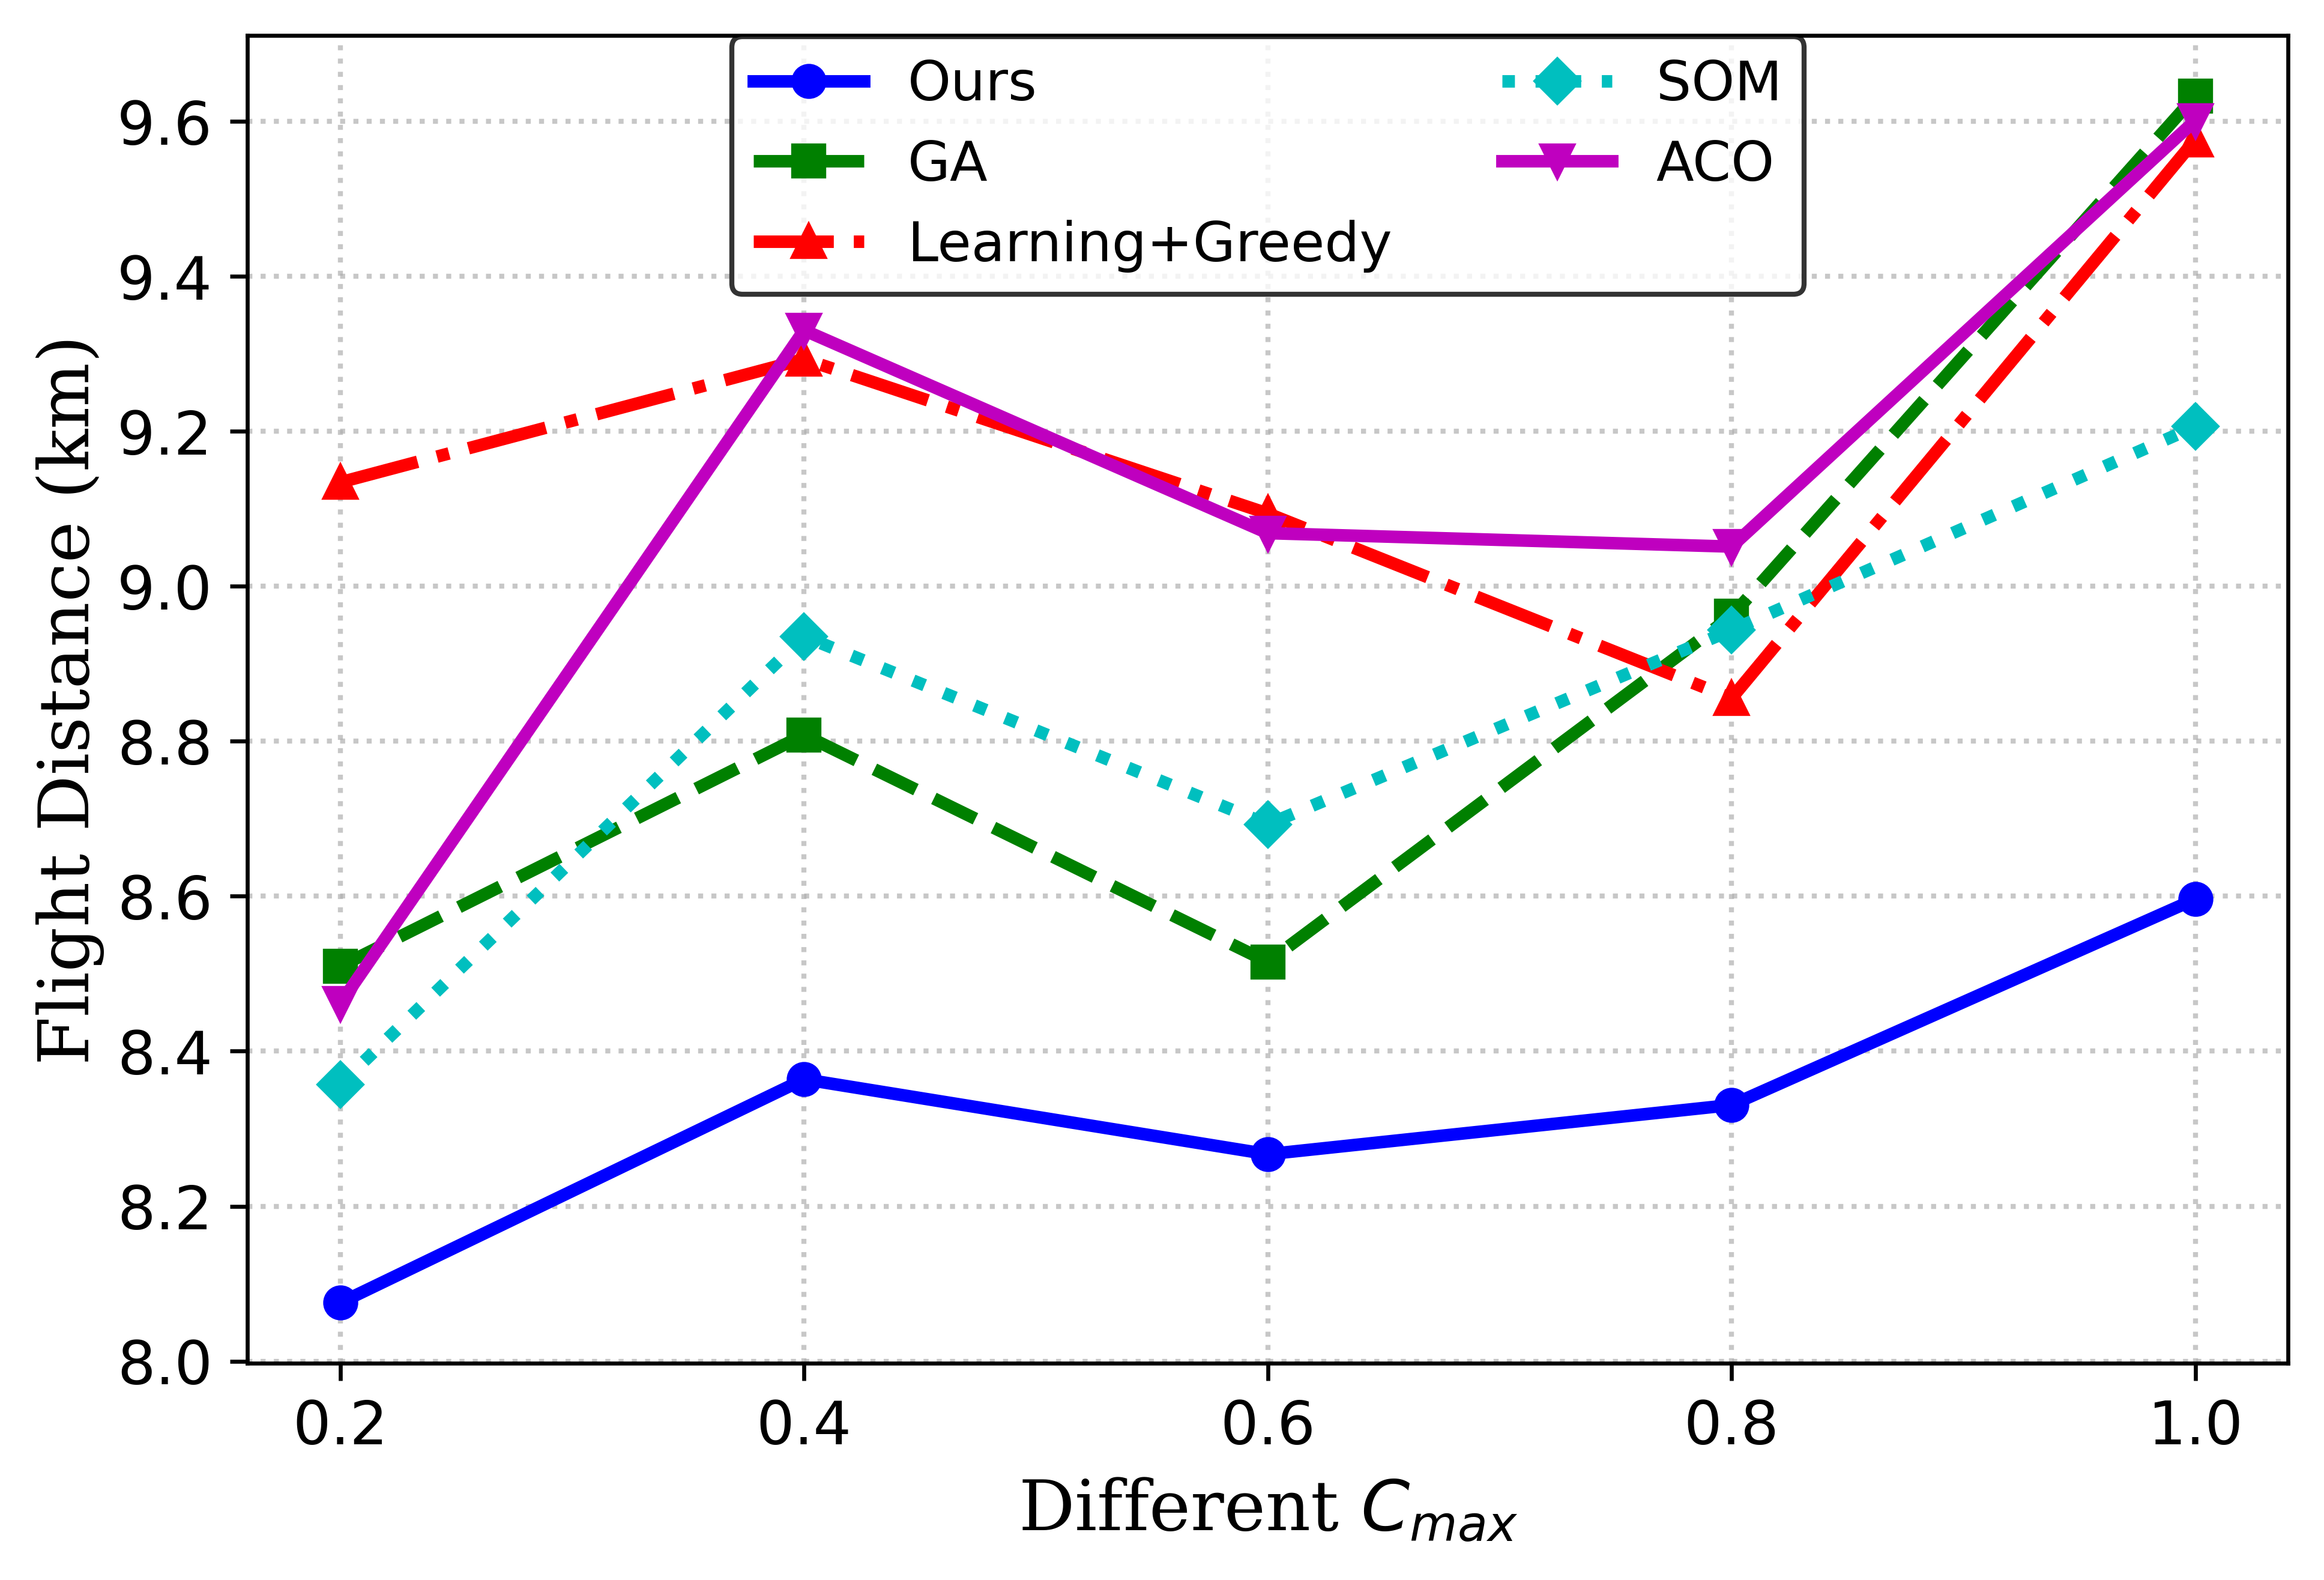
\includegraphics[width=0.3\linewidth]{fig/IEEE_不同搜索算法在不同cmax下的影响.png}
		\label{chutian3}
	}
	\caption{Performance impact of different $C_{max}$ values with $r_{com}=100$ and a network scale of 500.}
	\label{location}
\end{figure*}

This section evaluates the impact of parameter $C_{max}$ on system performance. As shown in Fig.~3a, the proposed method's effectiveness in suppressing redundant data varies with $C_{max}$. In small networks with dispersed IoT devices, $C_{max}$ has limited impact on redundant data reduction. However, as network size increases and device density grows, larger $C_{max}$ values significantly reduce redundant data collection during UAV operations. Fig.~3b demonstrates how increasing $C_{max}$ improves the network's redundant data suppression capability, consequently reducing total energy consumption across networks of 100, 300, and 500 nodes. The number of UAV waypoints increases proportionally with network size. Our comparative analysis in Fig.~3c confirms the algorithm's effectiveness in trajectory optimization. With 500 nodes and $C_{max}=1$, our method achieves the shortest flight distance, outperforming GA by 12.05\%, Learning+Greedy by 11.41\%, SOM by 7.09\%, and ACO by 11.69\%. %These results highlight our algorithm's significant advantage in optimizing flight trajectories, particularly in large-scale networks where efficiency improvements are most valuable.





\subsubsection{Comparative Analysis for Energy Efficiency}
%%%%%%%放置图片

\begin{figure*}[htbp]
	\centering
	\subfloat[Impact of different trajectory optimization algorithms.]{
		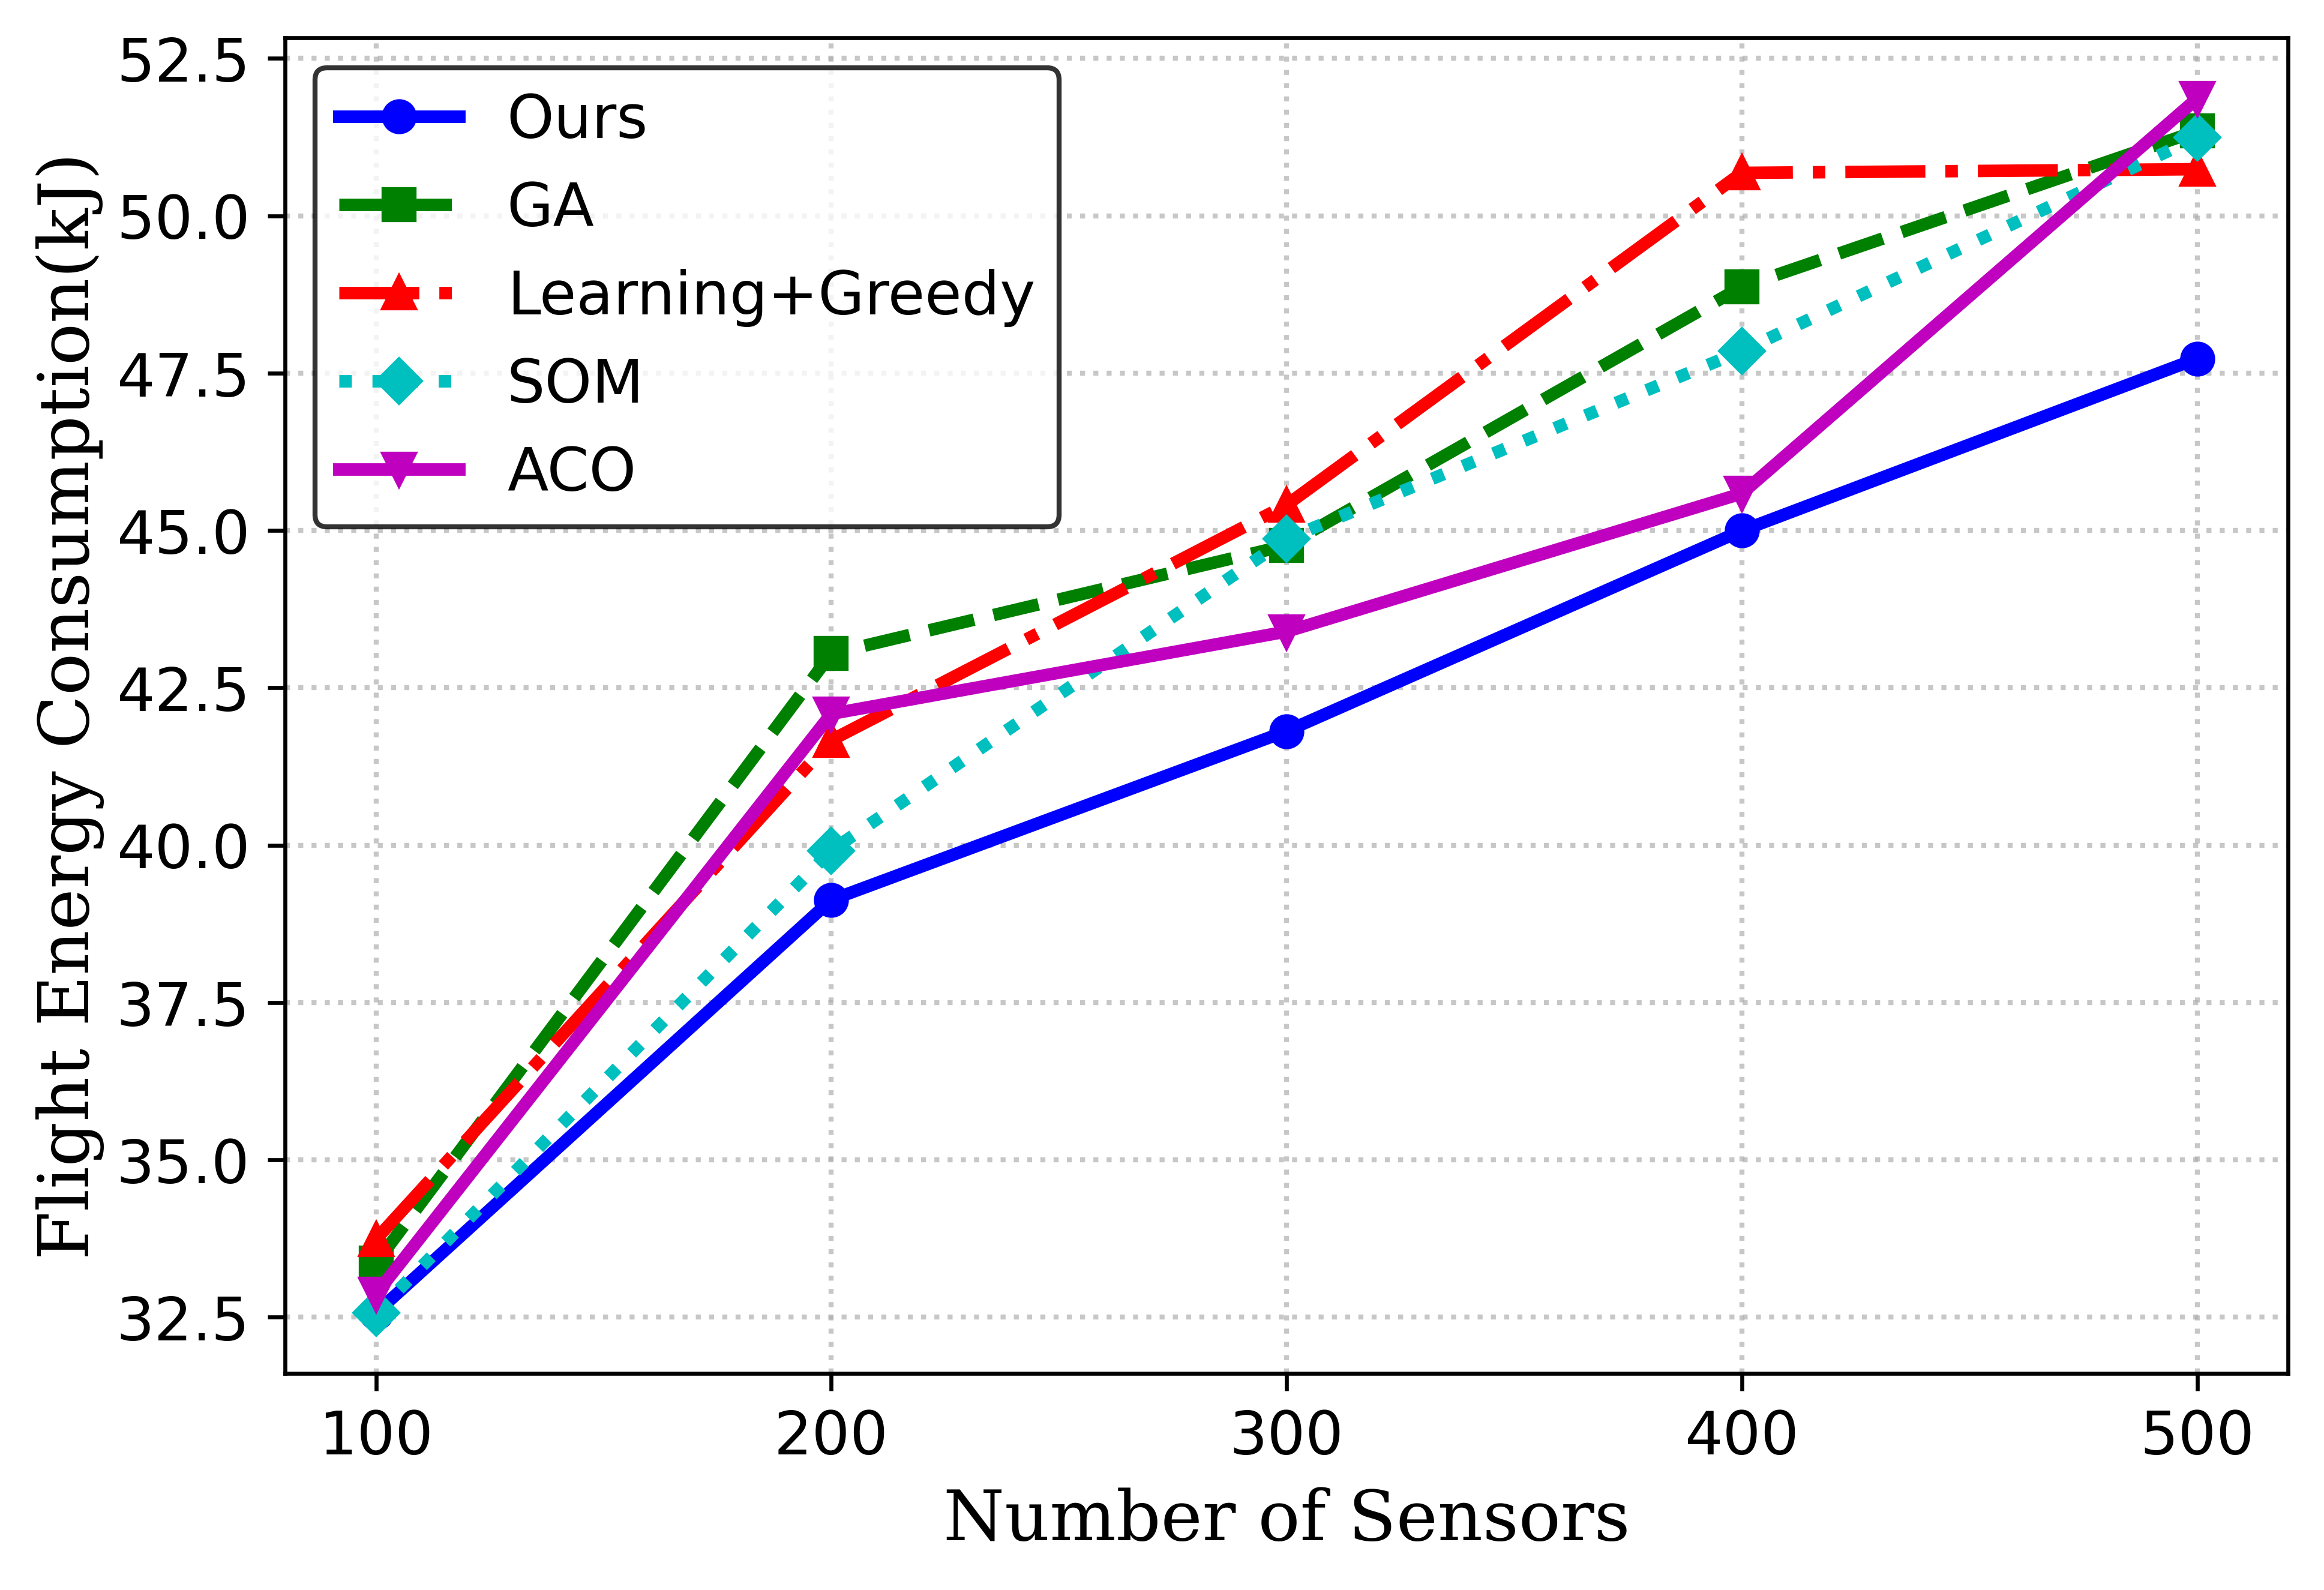
\includegraphics[width=0.45\linewidth]{fig/Different_Tra_Energy_Consumption.png}
		\label{chutian1}%文中引用该图片代号
	}
	\hfill
	\subfloat[Impact of different search strategies on the heatmap.]{

		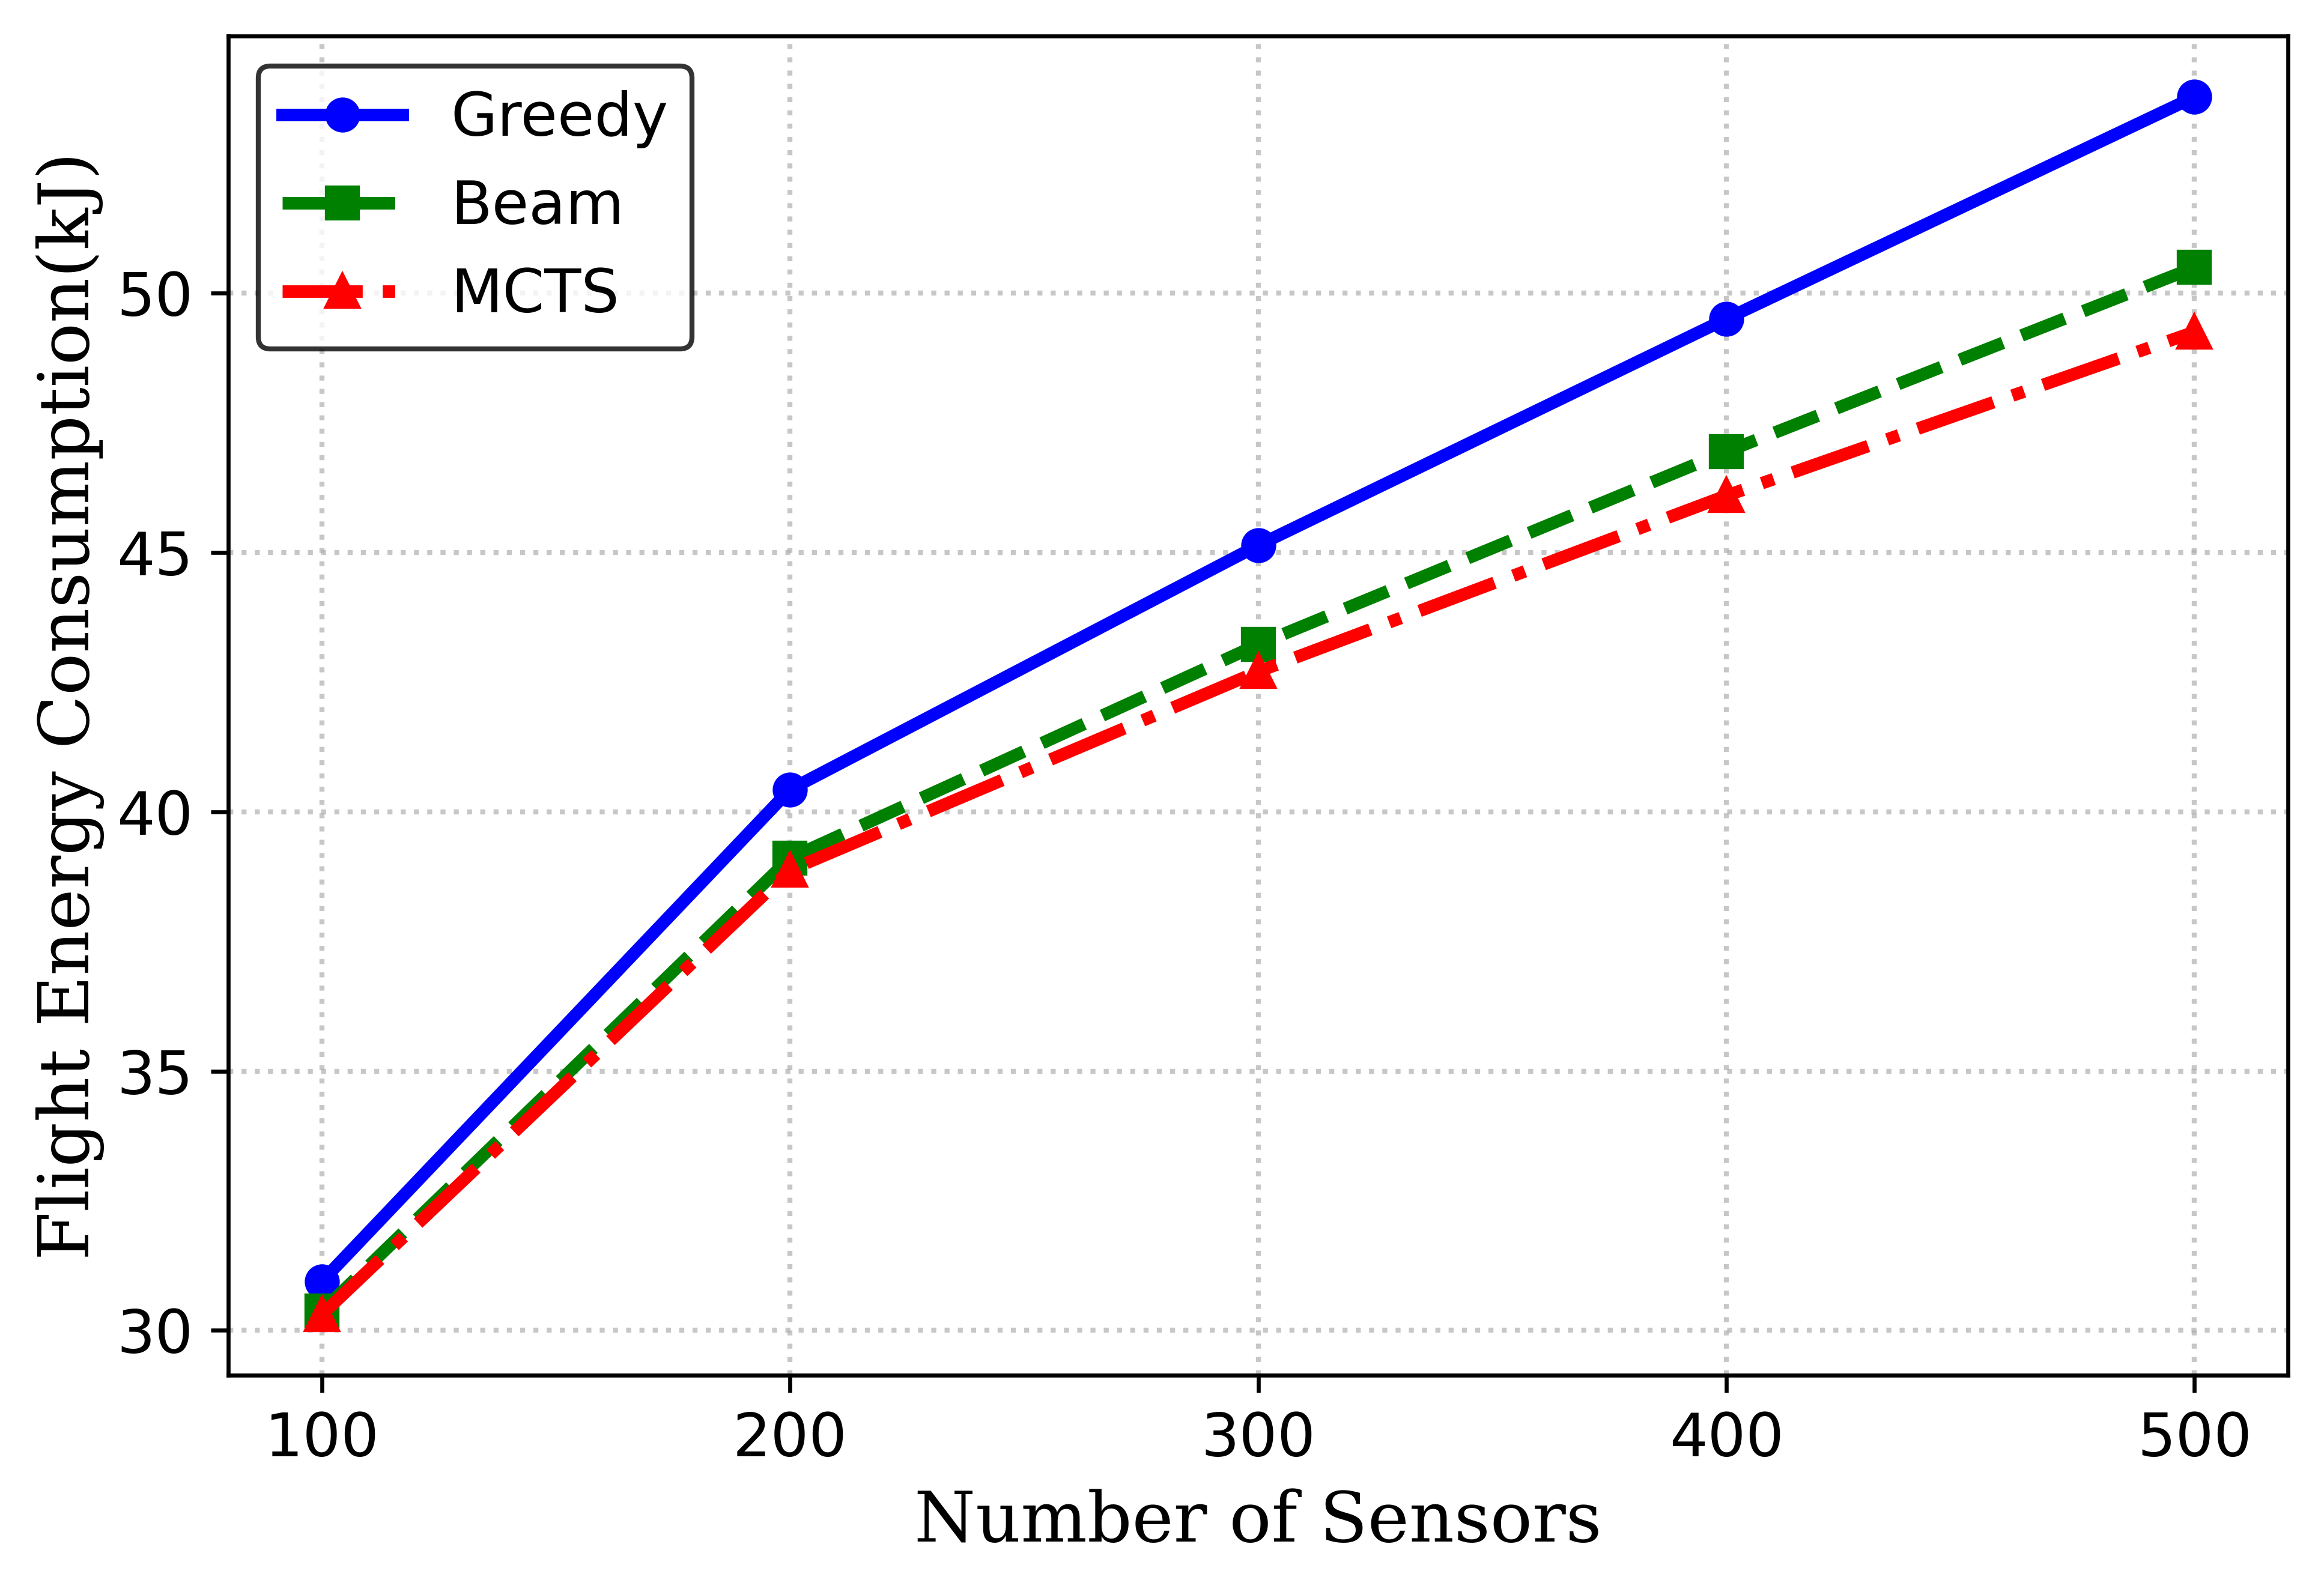
\includegraphics[width=0.45\linewidth]{fig/Different_Search_Energy_Consumption.png}
		\label{chutian2}%文中引用该图片代号
	}
    \caption{Performance impact of different optimization algorithms on flight energy consumption with $C_{max}=1$ and $r_{com} =100$.}
	\label{location} % 如果需要引用此图,可以使用这个标签
\end{figure*}


% 本节研究了不同路径规划算法和搜索策略对无人机飞行能耗的影响,实验在网络规模从100到500个节点的情况下进行,能耗以千焦(kJ)为单位衡量,分析了算法在不同规模网络下的能耗变化趋势。如图[Fig.4.a]所示,随着网络规模的增大,无人机的飞行能耗呈现上升趋势,这表明覆盖更大范围的网络需要更长的飞行路径。实验评估了我们提出的方法以及GA、Learning+Greedy、SOM和ACO等五种路径规划算法的性能。结果显示,我们的方法在所有网络规模下始终表现出最低的能耗,具有显著的优化效果。具体而言,与GA相比,我们的方法平均能耗降低了7.15%;与Learning+Greedy相比降低了7.92%;与SOM相比降低了4.21%;与ACO相比降低了4.66%。这些结果进一步验证了我们提出的路径规划算法在不同规模网络中的有效性,特别是在大规模场景下,能够显著降低无人机的飞行能耗,提高路径规划的优化能力。

% 除了路径规划算法,我们进一步分析了不同搜索策略对无人机飞行能耗的影响。实验对比了贪心搜索(Greedy Search)、束搜索(Beam Search)和我们提出的蒙特卡洛树搜索(MCTS)方法。如图[Fig.4.b]所示,随着网络规模的增加,三种搜索策略的能耗均呈上升趋势,这是由于更大规模的网络需要更多的悬停点和更长的飞行路径。实验结果表明,MCTS在所有搜索策略中表现出最优的能耗控制能力,相较于贪心搜索,其平均能耗降低了5.68%,相较于束搜索降低了1.28%。尽管不同策略的能耗有所差异,但我们提出的MCTS方法在所有评估的搜索策略中表现出最低的能耗,显示了其在大规模网络中的优势。

We evaluate trajectory optimization algorithms and search strategies for UAV energy consumption in networks of 100-500 nodes. As Fig.~4a shows, energy consumption increases with network size for all methods. Our proposed algorithm consistently outperforms GA, Learning+Greedy, SOM, and ACO across all network scales, reducing energy consumption by 7.15\%, 7.92\%, 4.21\%, and 4.66\% respectively. These results confirm our method's effectiveness, particularly in large-scale networks. We also compared search strategies including Greedy Search, Beam Search, and our proposed MCTS method. Fig.~4b demonstrates that while all strategies require more energy as network size increases, MCTS consistently achieves the lowest energy consumption, reducing it by 5.68\% compared to Greedy Search and 1.28\% compared to Beam Search. %This confirms MCTS's superior performance in large-scale network scenarios.



\subsubsection{Comparative Analysis for Communication Range}

\begin{figure*}[htbp]
	\centering
	\subfloat[Impact of different communication ranges on flight time.]{
		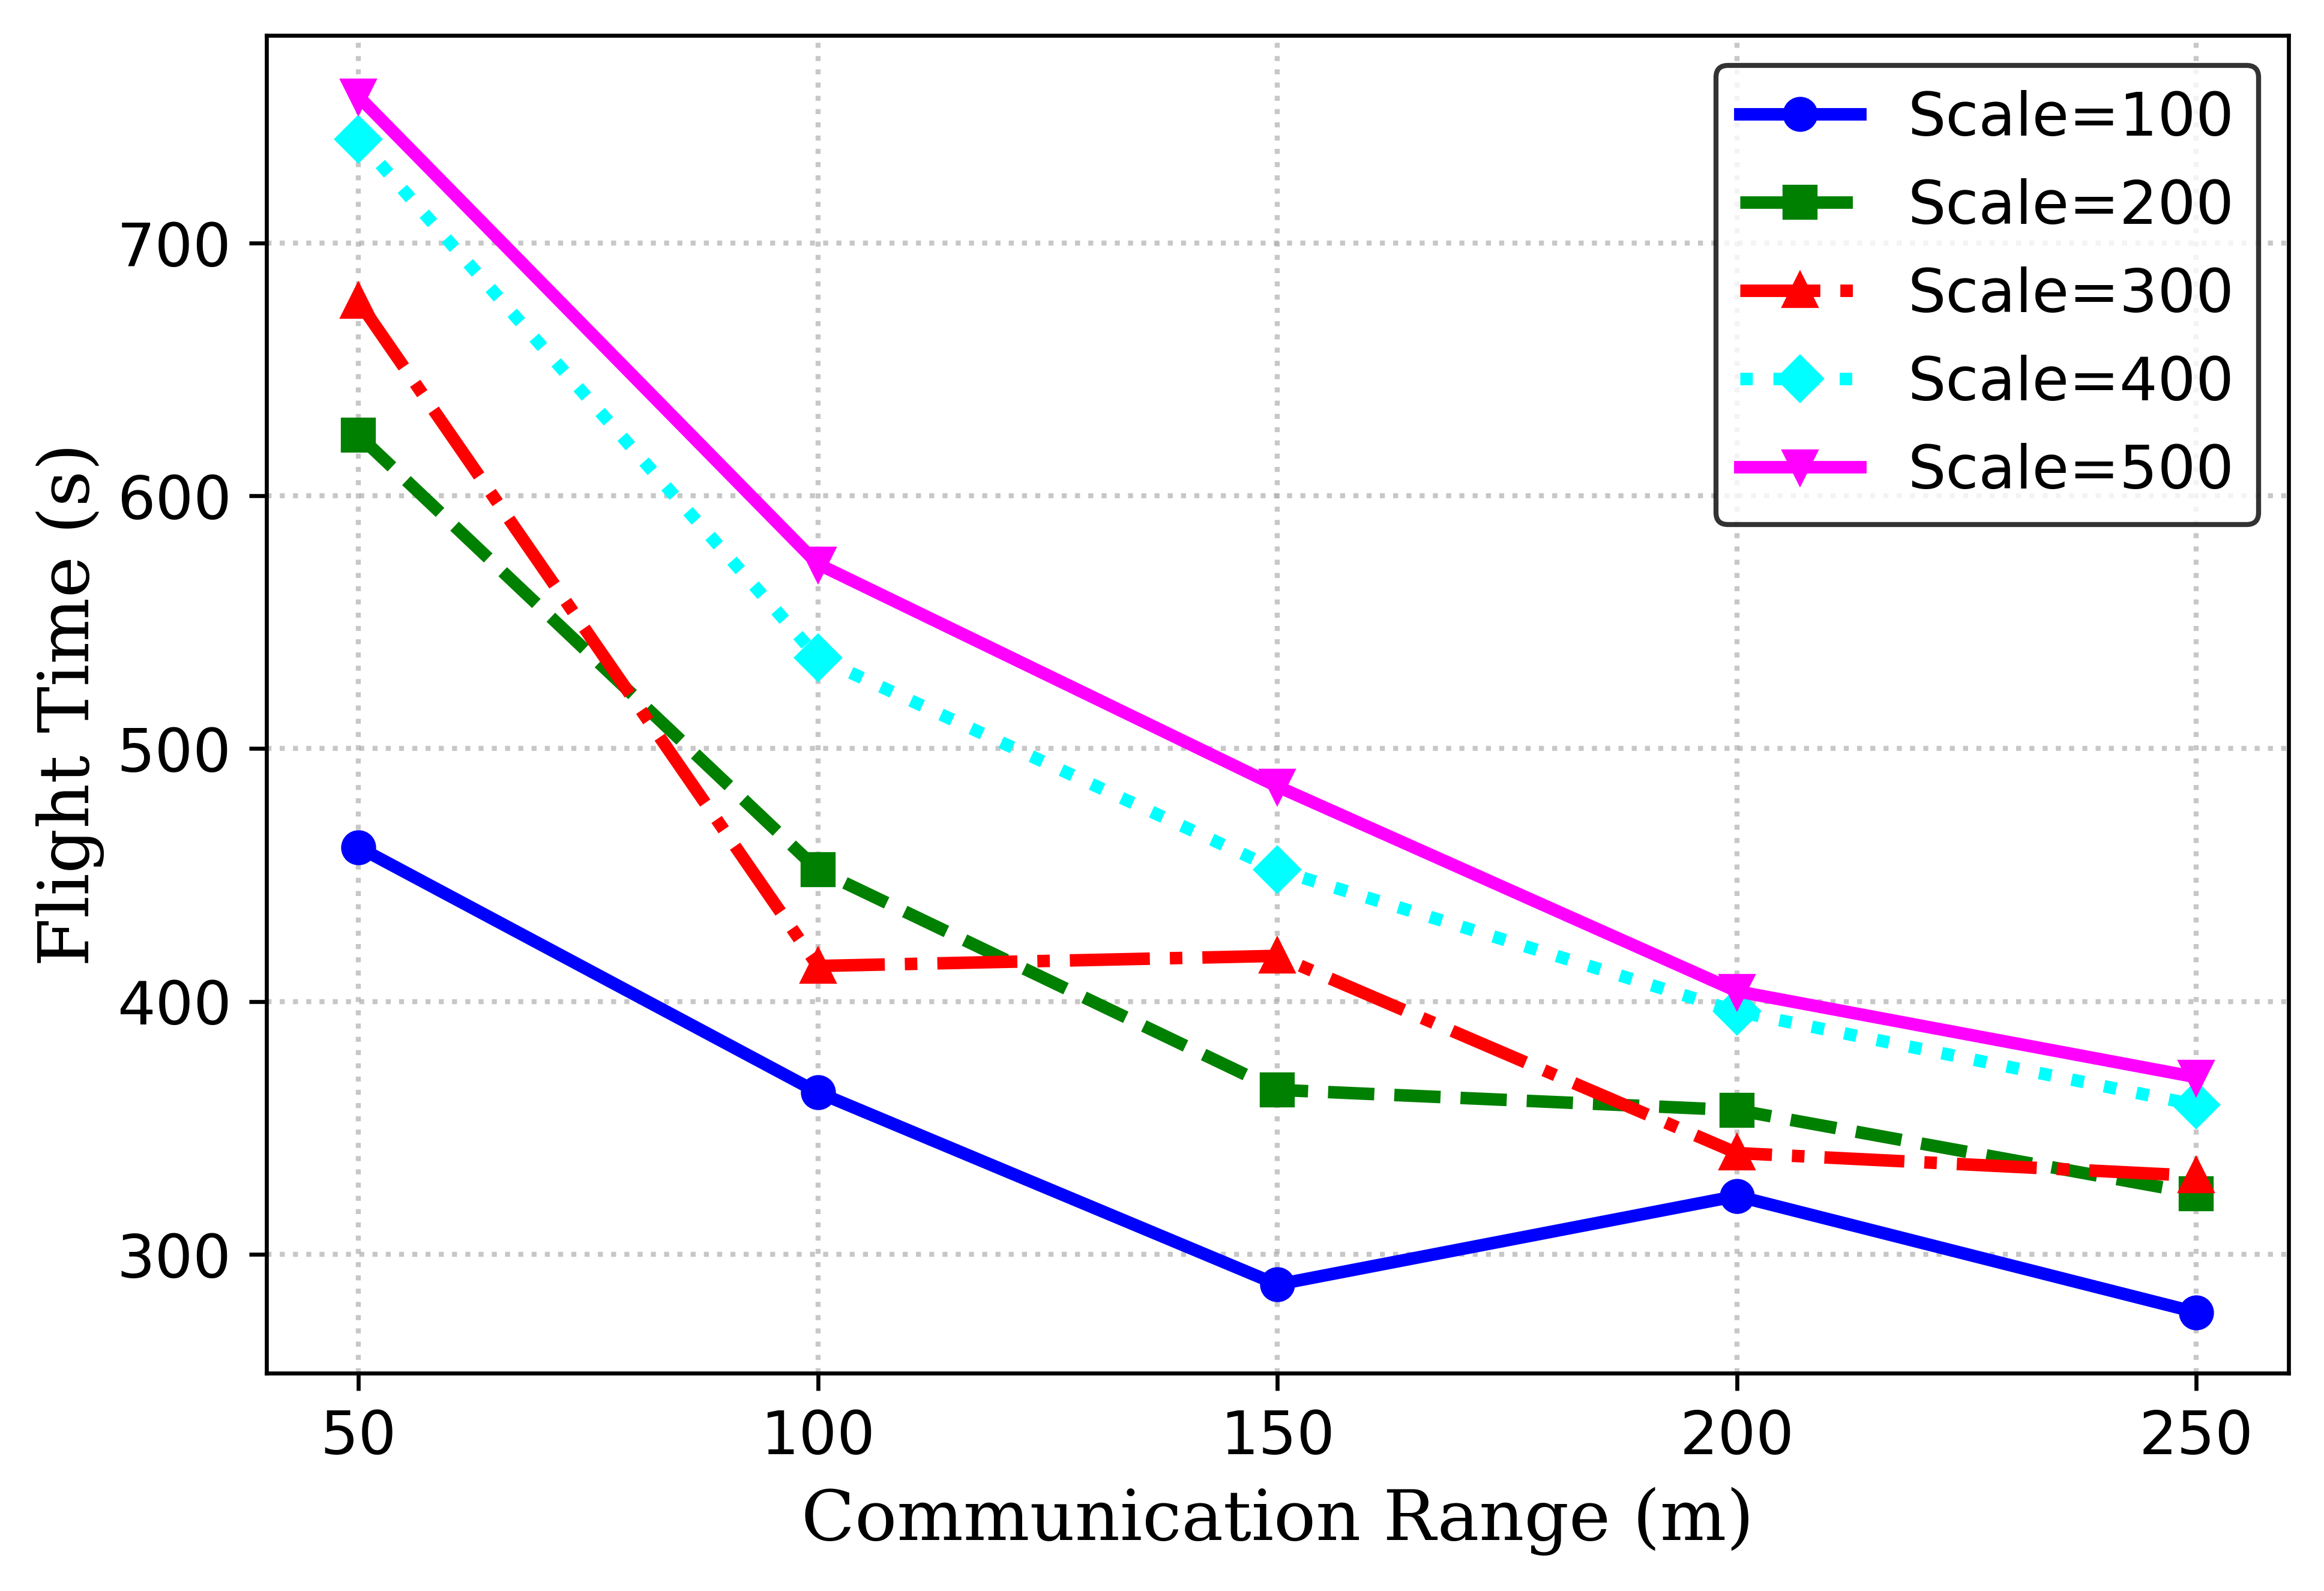
\includegraphics[width=0.31\linewidth]{fig/IEEE_传感器通信范围对飞行时间的影响.png}
		\label{chutian1}%文中引用该图片代号
	}
	\hfill
	\subfloat[Impact on the suppression of redundant data volume.]{
		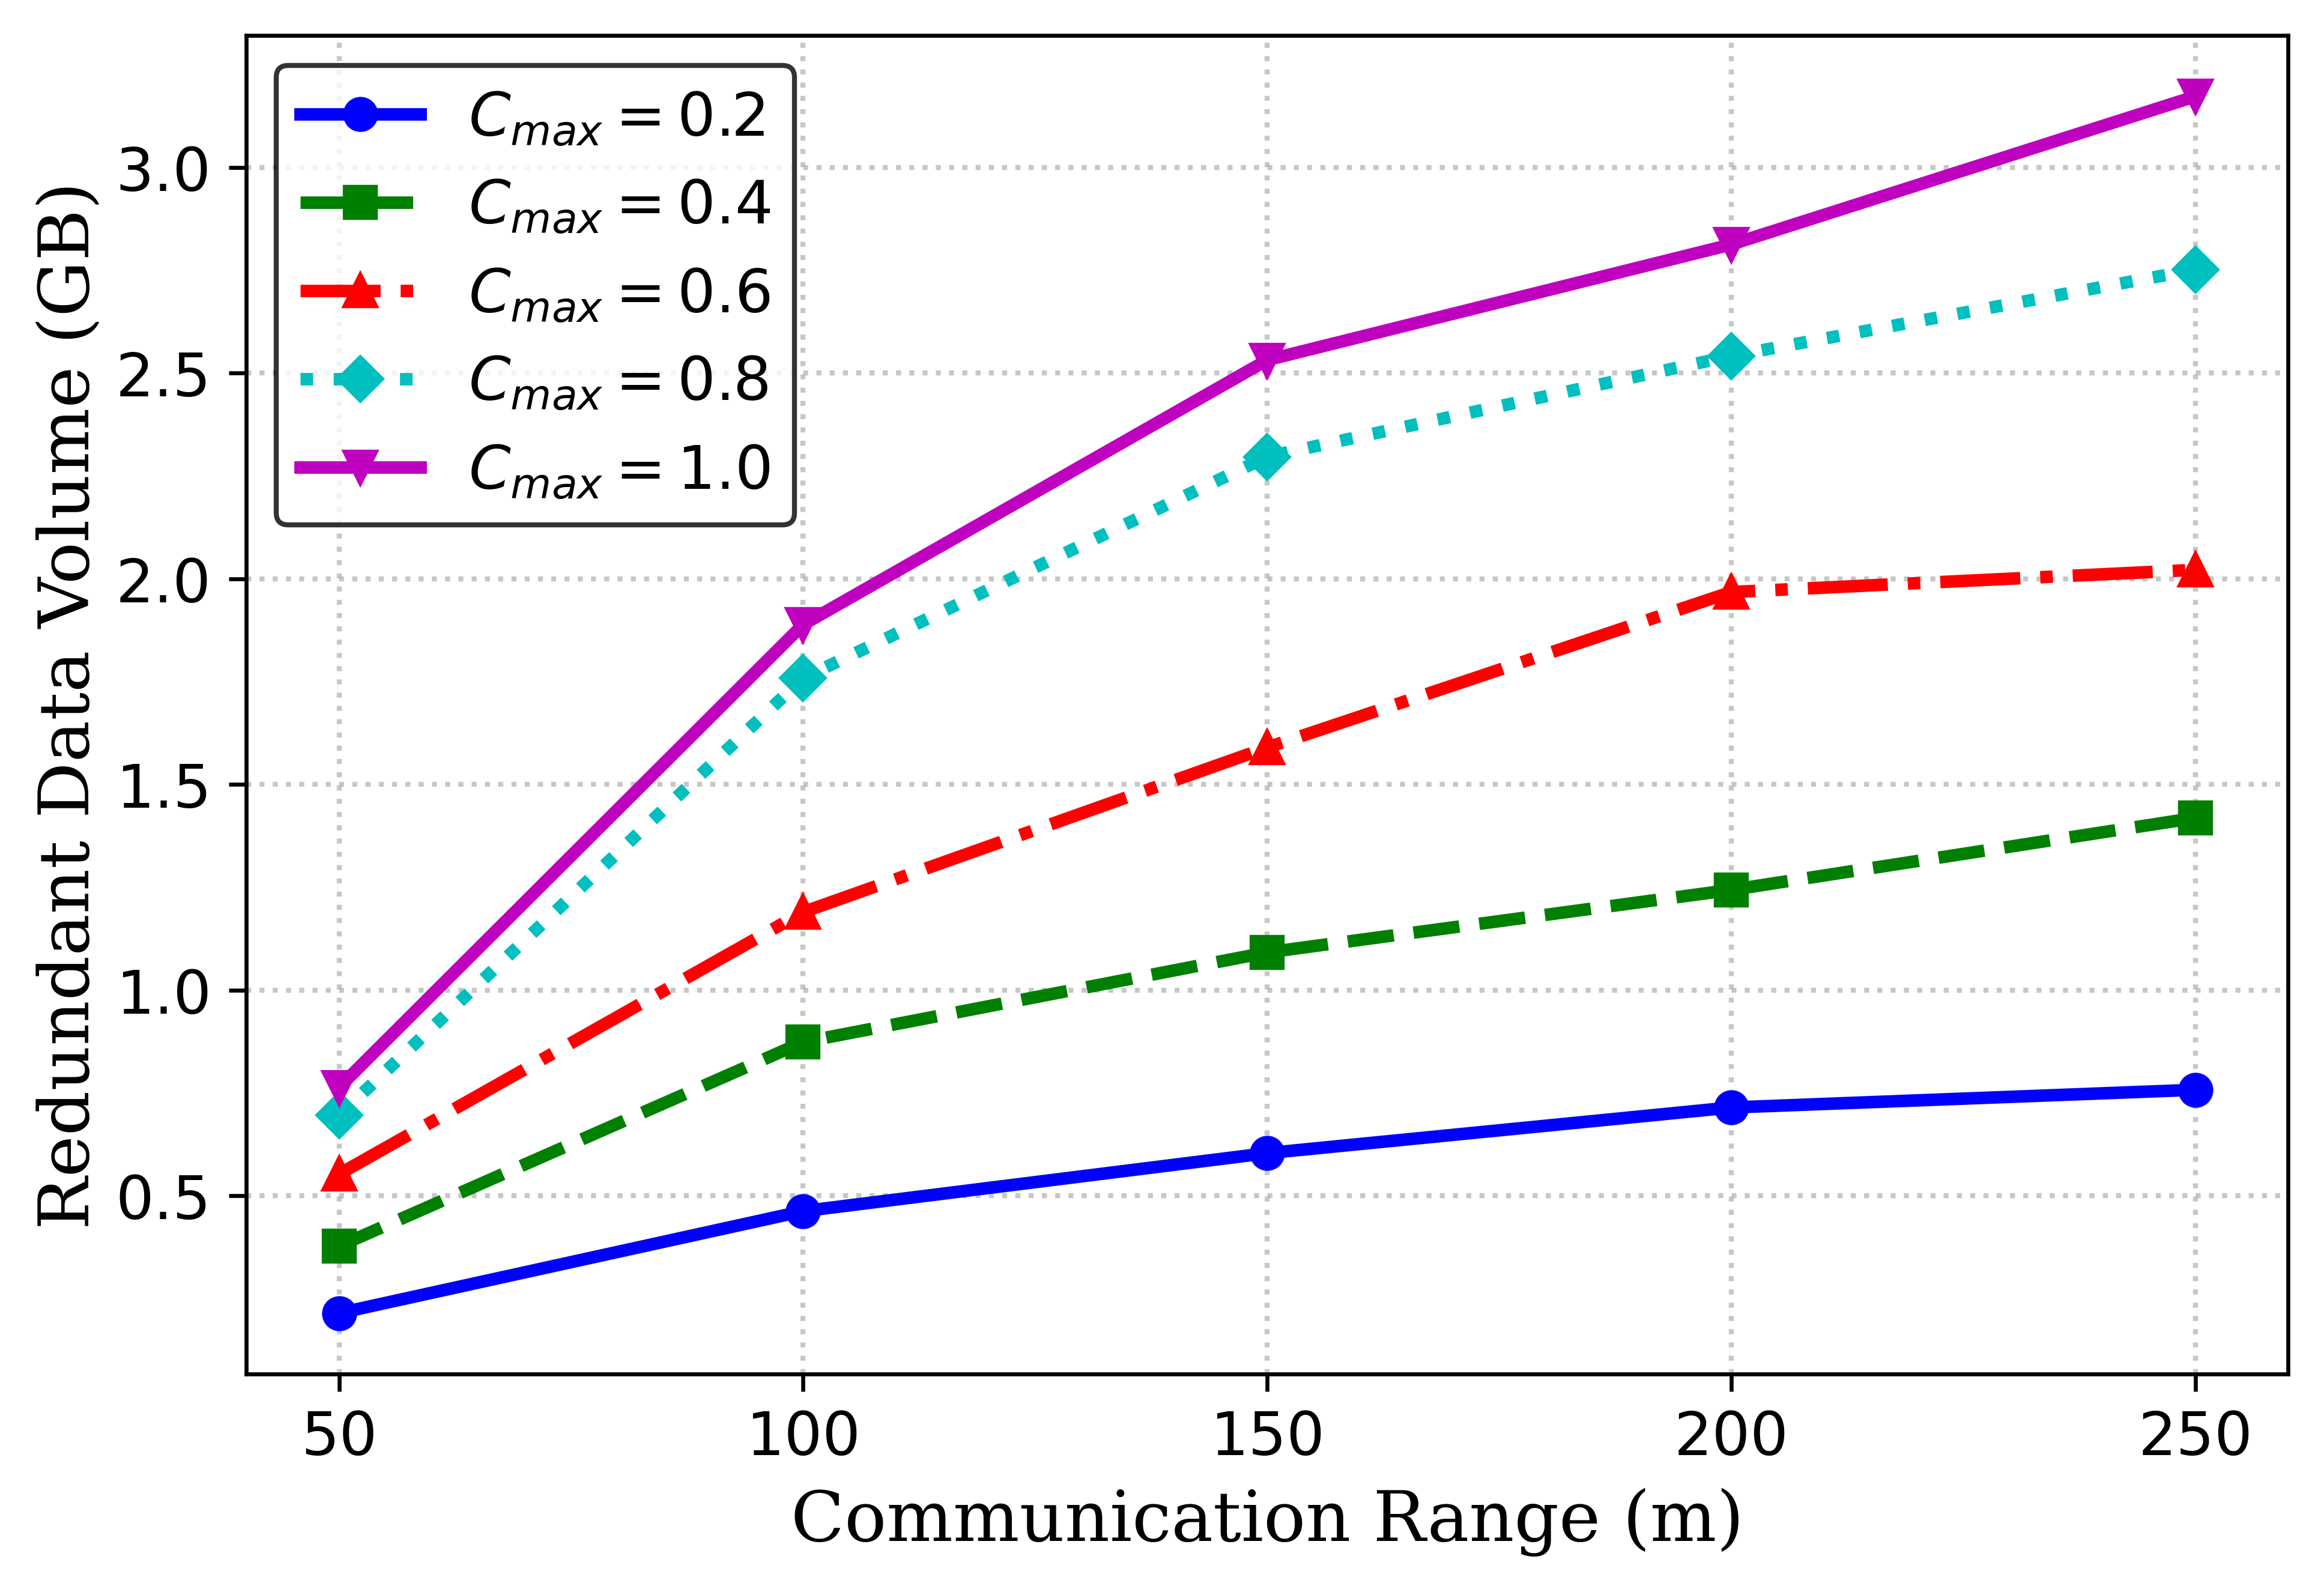
\includegraphics[width=0.31\linewidth]{fig/IEEE_通信范围对冗余数据量的影响.png}
		\label{chutian2}%文中引用该图片代号
	}
	\hfill
	\subfloat[Impact on total energy consumption.]{
		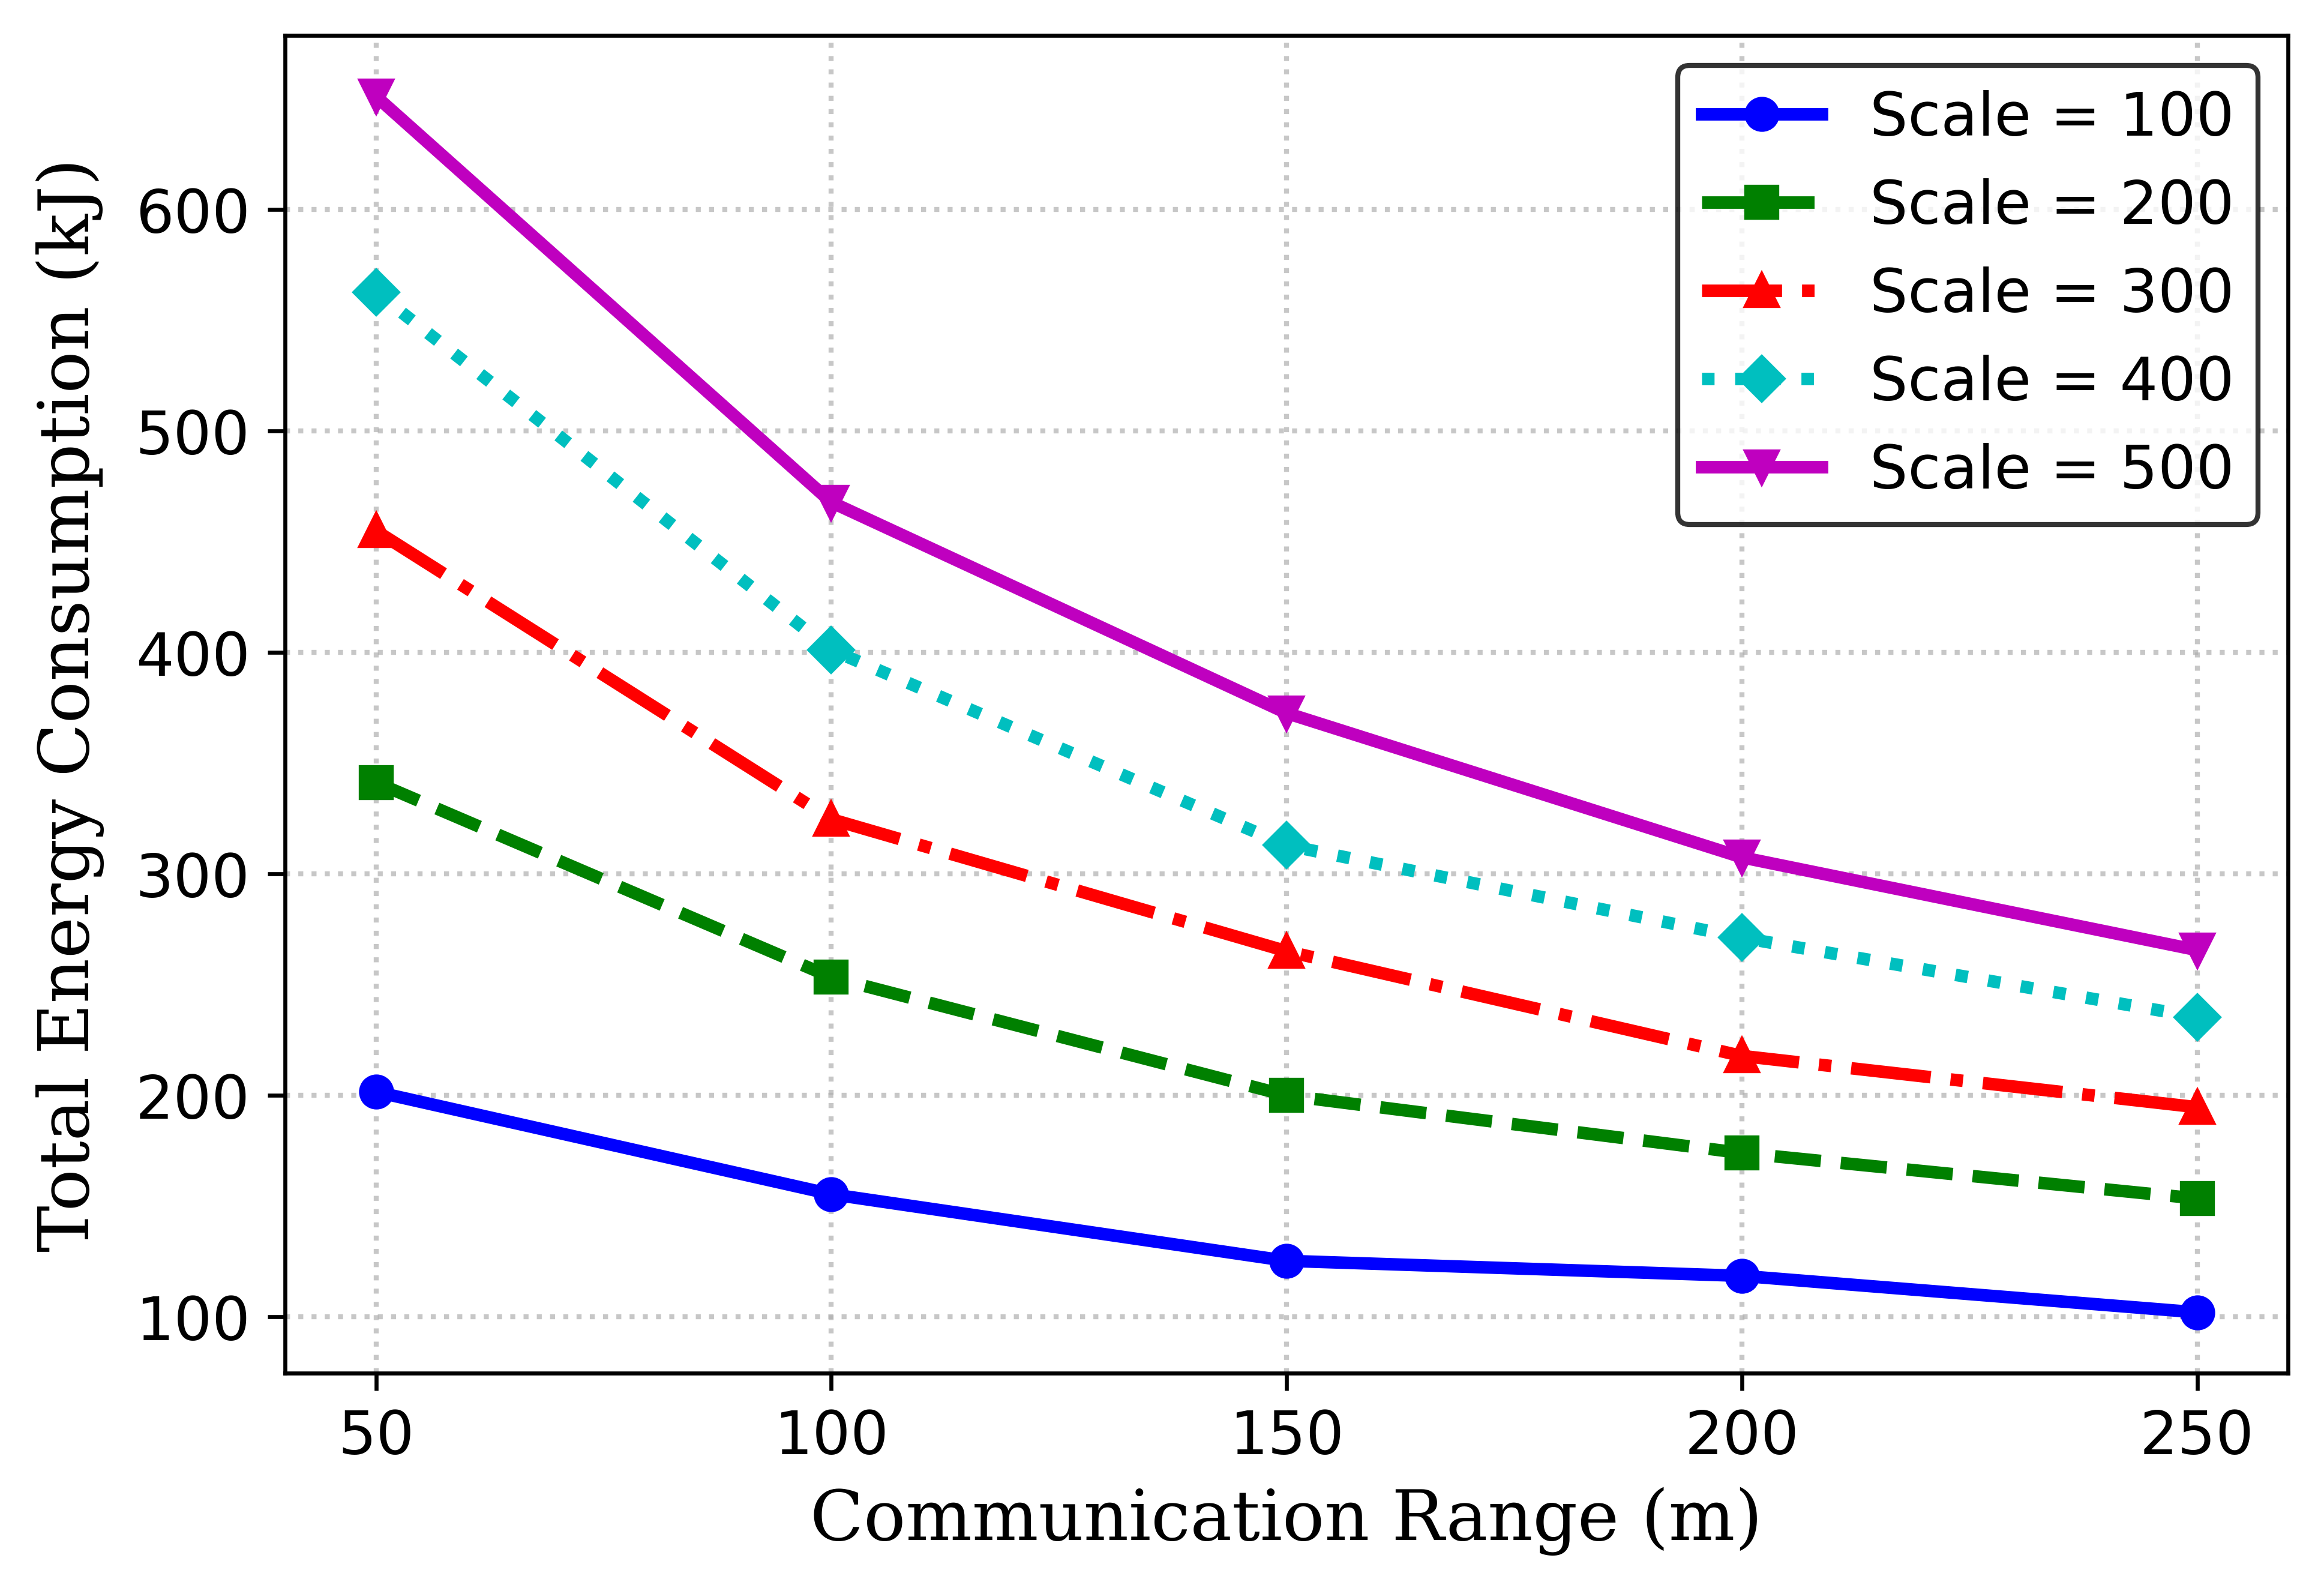
\includegraphics[width=0.31\linewidth]{fig/IEEE_传感器通信范围对总能耗影响.png}
		\label{chutian3}%文中引用该图片代号
	}
	\caption{Performance impact of different sensor communication ranges with a network scale of 100.}
	\label{location} % 如果需要引用此图,可以使用这个标签
\end{figure*}
%- 传感器节点不同通信范围的影响
% 为了研究传感器节点通信范围变化对系统性能的影响,我们分析了不同通信范围(50、100、150、200、250米)下冗余数据量、无人机飞行时间和总能量消耗的变化。实验结果如图[Fig9_a]、[Fig9_b]和[Fig9_c]所示,随着通信范围的增大,各项性能指标呈现出明显的变化趋势。

% 如图[Fig9_a]所示,增大传感器节点的通信范围会显著提高算法对冗余数据的抑制能力。这是因为较大的通信范围使得每个节点能够覆盖更广的区域,从而减少了数据重复传输的情况。图[Fig9_b]展示了通信范围对无人机飞行时间的影响。随着通信范围的增大,悬停点的数量减少,进而缩短了无人机的飞行时间,这表明较大的通信范围提高了数据采集效率。图[Fig9_c]则显示了通信范围对总能量消耗的影响。实验结果表明,较大的通信范围不仅减少了冗余数据的传输,还优化了无人机的飞行路径,显著降低了整体能量消耗。
We examined how IoT device communication range (50-250 meters) affects system performance. Fig.~5a-c show that increasing communication range significantly enhances redundant data suppression, as wider coverage reduces transmission redundancy. Consequently, larger communication ranges decrease the required UAV waypoints, reducing flight time (Fig.~5b) and optimizing collection efficiency. This improvement extends to total energy consumption (Fig.~5c), where expanded communication capabilities simultaneously minimize redundant data transmission and optimize flight paths, substantially lowering energy requirements.



\section{Related Work}
Research on data collection in UAV-assisted IoT networks has seen significant growth, with emphasis on simultaneously optimizing collection efficiency and energy consumption. Researchers in \cite{19-Multi-Objective_Ant_Colony_Optimization} proposed a multi-strategy multi-objective ant colony optimization algorithm that jointly designs aerial vehicle trajectories, hover positions, and speeds to minimize task completion time and energy while ensuring safety. Work in \cite{20-GPUDA} introduced a geometric partitioning-based dynamic programming algorithm, optimizing aerial vehicle paths by partitioning the IoT network and minimizing vehicle numbers under latency constraints. Authors in \cite{21-ROI} developed a region of interest partitioning and tracking strategy using mean-shift clustering and Voronoi diagrams to adapt to dynamic user distributions, enhancing network capacity and reducing energy consumption. However, these methods rely primarily on heuristics or mathematical programming, often experiencing exponential growth in computation time when applied to large-scale problems, limiting their practicality in real-world scenarios.



With advancements in machine learning, neural networks have been widely adopted to address these challenges. Research in \cite{22-minimizing_AOI} developed an aerial vehicle data collection framework for multi-cell networks, minimizing operational time and age of information using search-based and graph-based algorithms alongside deep reinforcement learning techniques. Authors in \cite{23-CMDP} designed an aerial vehicle-assisted wireless charging system for Internet of Things devices, employing constrained Markov decision processes and multi-agent constrained deep reinforcement learning to optimize trajectories while ensuring safety and service quality. Work in \cite{24-DDPG} proposed deep deterministic policy gradient and hybrid heuristic learning approaches to minimize mobile device energy consumption. Researchers in \cite{25-combinedRL_IL} combined reinforcement learning with imitation learning, training deep neural networks for collaborative aerial vehicle path planning to reduce task completion time and energy consumption. While these machine learning approaches demonstrate strong capabilities in handling complex wireless environments and learning efficient trajectory strategies, they still face limitations in generalization across problems of varying scales. %To address this issue, our work introduces techniques including graph sampling, graph transformation, and graph merging to enhance model adaptability and generalization ability. Additionally, our approach accounts for redundant data caused by overlapping coverage areas between adjacent nodes, further optimizing the efficiency of data collection.



\section{CONCLUSION}
%本文针对无人机辅助物联网数据收集的能量优化问题,提出了一种结合空间数据相关性与高质量路径规划的全新框架。该框架在数据冗余抑制方面,通过子模最大化建模,利用传感器数据的空间相似性进行聚类,并选取最佳的悬停点,以减少数据传输负担。在轨迹优化方面,我们将问题建模为旅行商问题 ,并采用图卷积神经网络与蒙特卡洛树搜索进行求解,以优化无人机飞行路径。最后,我们通过实验仿真评估了所提出算法的性能。仿真结果表明,这些算法能有效的降低无人机能耗,并在不同规模的问题上保持优良的求解质量和泛化能力。
This paper presents an energy optimization framework for UAV-assisted IoT data collection that uniquely integrates spatial data correlation analysis with trajectory optimization. By formulating redundancy suppression as a submodular maximization problem and employing Graph Convolutional Networks combined with Monte Carlo Tree Search for path optimization, our approach significantly reduces energy consumption while maintaining high solution quality across various problem scales. Extensive simulations using real-world sensor data demonstrate that our framework achieves up to 35\% energy savings compared to conventional approaches. Future work should address dynamic environments with mobile sensors, edge computing integration for real-time decision making, and coordination strategies for multi-UAV deployments to further enhance scalability and resilience in large-scale IoT networks.
% Limitations include assumptions of static IoT devices and inherent trade-offs between data freshness and collection efficiency. 

%%
%% The next two lines define the bibliography style to be used, and
%% the bibliography file.
\bibliographystyle{unsrt}
\bibliography{reference}



\end{document}
\endinput
%%
%% End of file `sample-sigconf.tex'.
